\documentclass{book}
\usepackage{a4wide}

%% possible fonts -- in order of preference
%%\usepackage{palatino}
\usepackage{bookman}
%%\usepackage{charter}
%%\usepackage{newcent}
%%\usepackage{times}
%%\usepackage{avant}
%%\usepackage{helvet}
%%\usepackage{sans}
%%\usepackage{chancery}

\usepackage[svgnames]{xcolor}	% for color text support
\usepackage[T1]{fontenc}
\usepackage[11pt]{moresize}
\usepackage{setspace}
\usepackage{ifpdf}
\usepackage{verbatim}   % for the comment environment
\usepackage{makeidx}
\usepackage{longtable}  %% page wrapping table environment
\usepackage{colortbl}   %% colors for tables
\usepackage{fancyvrb}   %% the "Verbatim" environment
\usepackage{fancyhdr}   %% custom headers and footers
\usepackage{multicol}
%% \usepackage{enumitem}   %% compact bullet lists with \begin{itemize}[noitemsep]
\usepackage{csquotes}   %% for the "displayquote" environment
\usepackage{listings}   %% source code listings with syntax highlight (lstxxx commands)
\usepackage[tight]{shorttoc}   %% for generating a second table of contents, only containing chapter titles
\usepackage{bytefield}  %% for drawing protocol frames
\usepackage{paralist}   %% for compact lists
\usepackage[nottoc]{tocbibind}  %% makes Bibliography and Index show up in TOC
\settocbibname{References}

\setlength{\textwidth}{160mm}
%\setlength{\oddsidemargin}{12.5mm}
%\setlength{\evensidemargin}{12.5mm}
%\setlength{\topmargin}{0mm}
\setlength{\textheight}{220mm}
%\setlength{\parskip}{1ex}
%\setlength{\parindent}{5ex}

\renewcommand{\bottomfraction}{0.9}
\renewcommand{\topfraction}{0.9}
\renewcommand{\floatpagefraction}{0.9}

\newenvironment{htmlonly}{\expandafter\comment}{\expandafter\endcomment}
\newcommand{\pdfonly}{}

%% try to cure overfull hboxes
%% \tolerance=500

%% for navigation in dvi files, only needed by old teTeX versions
%%\usepackage{srcltx}

%% try this for spell checking: cat ess2002.tex | ispell -l -t -a | sort | uniq | more

%%
%% The following snippet changes the horizontal spacing between the number and
%% the title in the table of contents.
%%
%% http://tex.stackexchange.com/questions/33841/how-to-modify-the-space-between-the-numbers-and-text-of-sectioning-titles-in-the
%%
\makeatletter
 \renewcommand*\l@section{\@dottedtocline{1}{2em}{3em}}
 \renewcommand*\l@subsection{\@dottedtocline{2}{5em}{4em}}
\renewcommand*\l@chapter[2]{%
  \ifnum \c@tocdepth >\m@ne
    \addpenalty{-\@highpenalty}%
    \vskip 1.0em \@plus\p@
    \setlength\@tempdima{2em}%
    \begingroup
      \parindent \z@ \rightskip \@pnumwidth
      \parfillskip -\@pnumwidth
      \leavevmode \bfseries
      \advance\leftskip\@tempdima
      \hskip -\leftskip
      #1\nobreak\hfil \nobreak\hb@xt@\@pnumwidth{\hss #2}\par
      \penalty\@highpenalty
    \endgroup
  \fi}
\makeatother

%%
%% OMNeT++ logo, use as {\opp}
%%
\makeatletter
%%\DeclareRobustCommand{\omnetpp}{OM\-NeT\kern-.18em++\@}
\DeclareRobustCommand{\omnetpp}{OMNeT++\@}
\makeatother

\newcommand{\opp}{\omnetpp}

%%
%% PDF Header
%%
% note: \ifpdf now comes from the ifpdf package
%\newif\ifpdf
%\ifx\pdfoutput\undefined
%  \pdffalse
%\else
%  \pdfoutput=1
%  \pdftrue
%\fi
%% PDF-Info
\ifpdf
  \usepackage[pdftex]{graphicx}
  \usepackage[plainpages=false,linktocpage,bookmarksnumbered=true,pdftex]{hyperref}   %% automatic hyperlinking
  \pdfcompresslevel=9
  \pdfinfo{/Author (Andras Varga and others)
    /Title (INET Framework User's Guide)
    /Subject ()
    /Keywords (INET, INETMANET, OMNeT++, manual)}
\else
  \usepackage{graphicx}
  \usepackage[plainpages=false]{hyperref}   %% automatic hyperlinking
\fi

%%
%% Draft conditional to include unfinished parts
%%
\newif\ifdraft
\draftfalse %% uncomment for final version
%\drafttrue %% uncomment for draft version

%%
%% Generate Index
%%
\makeindex


%%
%% Link colors (hyperref package)
%%
\definecolor{MyDarkBlue}{rgb}{0.16,0.16,0.5}
%% XXX the next line apparently screws up all links except in TOC! they'll be colored nicely, but won't work.
%\hypersetup{
%    colorlinks=true,
%    linkcolor=MyDarkBlue,
%    anchorcolor=MyDarkBlue,
%    citecolor=MyDarkBlue,
%    filecolor=MyDarkBlue,
%    menucolor=MyDarkBlue,
%    runcolor=MyDarkBlue,
%    urlcolor=blue,
%}

%%
%% Heading and Footer
%%
\pagestyle{fancy}
\fancyhf{}
\renewcommand{\footrulewidth}{0.5pt}
\renewcommand{\chaptermark}[1]{\markboth{#1}{}}
\lhead{INET Framework User's Guide -- \leftmark}
\rfoot{\thepage}

%% this is used for chapter start pages
\fancypagestyle{plain}{
    \rfoot{\thepage}
}

%%
%% Use \begin{graybox}...\end{graybox} for notes
%%
\definecolor{MyGray}{rgb}{0.85,0.85,1.0}
\makeatletter\newenvironment{graybox}%
   {\begin{flushright}\begin{lrbox}{\@tempboxa}\begin{minipage}[r]{0.95\textwidth}}%
   {\end{minipage}\end{lrbox}\colorbox{MyGray}{\usebox{\@tempboxa}}\end{flushright}}%
\makeatother


\newenvironment{note}{\begin{graybox}\textbf{NOTE: }}{\end{graybox}}
\newenvironment{hint}{\begin{graybox}\textbf{HINT: }}{\end{graybox}}
\newenvironment{warning}{\begin{graybox}\textbf{WARNING: }}{\end{graybox}}
\newenvironment{caution}{\begin{graybox}\textbf{CAUTION: }}{\end{graybox}}
\newenvironment{rationale}{\begin{graybox}\textbf{Rationale: }}{\end{graybox}}
\newenvironment{important}{\begin{graybox}\textbf{IMPORTANT: }}{\end{graybox}}

%%
%% Set up listings package
%%
\lstloadlanguages{C++,make,perl,tcl,XML,R,Matlab}

%% See listings.pdf,pp20
\lstdefinelanguage{NED} {
    morekeywords={allowunconnected,bool,channel,channelinterface,connections,const,
                  default,double,extends,false,for,gates,if,import,index,inout,input,
                  int,like,module,moduleinterface,network,output,package,parameters,
                  property,simple,sizeof,string,submodules,this,true,types,volatile,
                  xml,xmldoc},
    sensitive=true,
    morecomment=[l]{//},
    morestring=[b]",
}
\lstdefinelanguage{MSG} {
    morekeywords={abstract,bool,char,class,cplusplus,double,enum,extends,false,
                  fields,int,long,message,namespace,noncobject,packet,properties,
                  readonly,short,string,struct,true,unsigned},
    sensitive=true,
    morecomment=[l]{//},
    morestring=[b]",
}
\lstdefinelanguage{inifile} {
    morekeywords={},
    sensitive=true,
    morecomment=[l]{\#},
    morestring=[b]",
}
\lstdefinelanguage{pseudocode} {
    morekeywords={if,then,else,otherwise,whenever,while},
    sensitive=true,
    morecomment=[l]{//},
    morestring=[b]",
    mathescape=true,
}

%% thick ruler on the left; also, designate backtick as LaTeX escape character
%% (e.g. \opp needs to be written as `\opp` inside listing blocks)
\lstset{
    escapechar=`,
    basicstyle=\ttfamily,
    identifierstyle=\color{Black},
    stringstyle=\color{DarkBlue},
    commentstyle=\color{SeaGreen},
    keywordstyle=\bfseries\color{Purple},
    showstringspaces=false,
    frame=leftline,
    framesep=10pt,
    framerule=3pt,
    xleftmargin=15pt
}

\definecolor{NEDRulerColor}{rgb}{0.5,1.0,0.5}  % pale green
\definecolor{MSGRulerColor}{rgb}{0.5,1.0,0.5}  % pale green
\definecolor{CPPRulerColor}{rgb}{0.8,0.5,0.2}  % pale orange
\definecolor{IniRulerColor}{rgb}{0.9,0.9,0.3}  % pale yellow
\definecolor{FileListingRulerColor}{rgb}{0.85,0.85,0.85}  % grey
%\definecolor{CommandLineRulerColor}{rgb}{0.9,0.9,0.2}
\definecolor{PseudoCodeRulerColor}{rgb}{0.0,1.0,1.0}  % cyan
\definecolor{XMLRulerColor}{rgb}{0.8,0.8,1.0}  % pale blue

%% See listings.pdf,pp39
\lstnewenvironment{ned}
    {\lstset{language=NED,rulecolor=\color{NEDRulerColor}}}
    {}
\lstnewenvironment{msg}
    {\lstset{language=MSG,rulecolor=\color{MSGRulerColor}}}
    {}
\lstnewenvironment{cpp}
    {\lstset{language=C++,rulecolor=\color{CPPRulerColor}}}
    {}
\lstnewenvironment{inifile}
    {\lstset{language=inifile,rulecolor=\color{IniRulerColor}}}
    {}
\lstnewenvironment{filelisting}
    {\lstset{language={},rulecolor=\color{FileListingRulerColor}}}
    {}
\lstnewenvironment{commandline}
    {\lstset{language={},framesep=11pt,framerule=1pt,xleftmargin=16pt}}
    {}
\lstnewenvironment{pseudocode}
    {\lstset{language=pseudocode,rulecolor=\color{PseudoCodeRulerColor}}}
    {}
\lstnewenvironment{XML}
    {\lstset{language=XML,rulecolor=\color{XMLRulerColor}}}
    {}

% add caption={#2} to display caption
\newcommand{\xmlsnippet}[2]{%
    \lstinputlisting[language=XML,rulecolor=\color{XMLRulerColor},linerange=<!\-\-#1\-\->-<!\-\-End\-\->,includerangemarker=false,firstnumber=0]{Snippets.xml}}
\newcommand{\cppsnippet}[2]{%
    \lstinputlisting[language=C++,rulecolor=\color{CPPRulerColor},linerange=//!#1-//!End,includerangemarker=false,firstnumber=0]{Snippets.cc}}
\newcommand{\msgsnippet}[2]{%
    \lstinputlisting[language=msg,rulecolor=\color{MSGRulerColor},linerange=//!#1-//!End,includerangemarker=false,firstnumber=0]{Snippets.msg}}
\newcommand{\nedsnippet}[2]{%
    \lstinputlisting[language=ned,rulecolor=\color{NEDRulerColor},linerange=//!#1-//!End,includerangemarker=false,firstnumber=0]{Snippets.ned}}
\newcommand{\inisnippet}[2]{%
    \lstinputlisting[language=inifile,rulecolor=\color{IniRulerColor},linerange=\#!#1-\#!End,includerangemarker=false,firstnumber=0]{Snippets.ini}}

%%
%% some customization
%%
\setlength{\parindent}{0pt}
\setlength{\parskip}{1ex}

%%
%% Shortcuts
%%
\newcommand{\appendixchapter}{\chapter} %% html converter needs to know which chapters are appendices

\newcommand{\tbf}{\textbf} %% bold faced text
\newcommand{\ttt}{\texttt} %% type writer font text

\newcommand{\tab}{\hspace*{5mm}} %% tabulator settings

\newcommand{\new}{$^{New!}$}
\newcommand{\changed}{$^{Changed!}$}

\newcommand{\program}{\textbf}

\newcommand{\includepng}{\includegraphics}
\newcommand{\includesvg}{\includegraphics}

%% Colordefinition for table header rows (requires package colortbl)
\newcommand{\tabheadcol}{\rowcolor[gray]{0.8}}

%%
%% Function/Class/Macro/Variable/Program/Parameter/Define names
%%
%% Write the names in type writer font and do an index entry
%% Allows word wrap by automatic hyphenation
%%
%% Usage: \ffunc{take()}
%%    or: \ffunc[take()]{take(obj)}
%% the second form uses the bracketed word for the index entry
%%

\newcommand{\protocol}[1]{%
    {#1}}

%% NED type names
\newcommand{\nedtype}[2][\DefaultOpt]{\def\DefaultOpt{#2}%
  \index{#1}%
  \texttt{\hyphenchar\font=`\-\relax#2}}

%% MSG type names
\newcommand{\msgtype}[2][\DefaultOpt]{\def\DefaultOpt{#2}%
  \index{#1}%
  \texttt{\hyphenchar\font=`\-\relax#2}}

%% Function names
\newcommand{\ffunc}[2][\DefaultOpt]{\def\DefaultOpt{#2}%
  \index{#1}%
  \texttt{\hyphenchar\font=`\-\relax#2}}

%% Class names
\newcommand{\cppclass}[2][\DefaultOpt]{\def\DefaultOpt{#2}%
  \index{#1}%
  \texttt{\hyphenchar\font=`\-\relax#2}}

%% Macro names
\newcommand{\fmac}[2][\DefaultOpt]{\def\DefaultOpt{#2}%
  \index{#1}%
  \texttt{\hyphenchar\font=`\-\relax#2}}

%% Variable names
\newcommand{\fvar}[2][\DefaultOpt]{\def\DefaultOpt{#2}%
  \index{#1}%
  \texttt{\hyphenchar\font=`\-\relax#2}}

%% Program names
\newcommand{\fprog}[2][\DefaultOpt]{\def\DefaultOpt{#2}%
  \index{#1}%
  \texttt{\hyphenchar\font=`\-\relax#2}}

%% Parameter names
\newcommand{\fpar}[2][\DefaultOpt]{\def\DefaultOpt{#2}%
  \index{#1}%
  \texttt{\hyphenchar\font=`\-\relax#2}}

%% Defines
\newcommand{\fdef}[2][\DefaultOpt]{\def\DefaultOpt{#2}%
  \index{#1}%
  \texttt{\hyphenchar\font=`\-\relax#2}}

%% NED/MSG properties
\newcommand{\fprop}[2][\DefaultOpt]{\def\DefaultOpt{#2}%
  \index{#1}%
  \texttt{\hyphenchar\font=`\-\relax#2}}

%% Keywords (NED, MSG)
\newcommand{\fkeyword}[2][\DefaultOpt]{\def\DefaultOpt{#2}%
  \index{#1}%
  \textbf{\texttt{\hyphenchar\font=`\-\relax#2}}}

%% Configuration options
\newcommand{\fconfig}[2][\DefaultOpt]{\def\DefaultOpt{#2}%
  \index{#1}%
  \textbf{\texttt{\hyphenchar\font=`\-\relax#2}}}

%% File names
\newcommand{\ffilename}[2][\DefaultOpt]{\def\DefaultOpt{#2}%
  \index{#1}%
  \texttt{\hyphenchar\font=`\-\relax#2}}

%% Signals
\newcommand{\fsignal}[2][\DefaultOpt]{\def\DefaultOpt{#2}%
  \index{#1}%
  \texttt{\hyphenchar\font=`\-\relax#2}}

\newcommand{\fgate}[1]{\texttt{\hyphenchar\font=`\-\relax#1}}

%% do not number subsubsections
%\setcounter{secnumdepth}{4}

% limit the depth of TOC
\setcounter{tocdepth}{2}

%%
%% Start of document
%%
\begin{document}

%% set the image type preference
\DeclareGraphicsExtensions{.pdf,.png}

\pagestyle{empty}
\pagenumbering{roman}

%% %%\begin{figure}[htbp]
%%\begin{center}
%%\includegraphics[width=3.648in, height=0.990in]{figures/usmanFig1}
%%\end{center}
%% %%\end{figure}

%% the following {center} is a trick -- vspace does nothing if there's
%% nothing above it in the page
\begin{center}\end{center}
\vspace{16em}
\hrule
\vspace{2em}
\begin{center}
{\HUGE INET Framework}\\
\vspace{2em}
{\Huge Developer's Guide}\\
\vspace{2em}
{\Large Version 4.0}\\
\end{center}
\vspace{2em}
\hrule

\begin{center}
\textit{\today}
\end{center}




\cleardoublepage

%%\setcounter{page}{1}
%\newpage
%%\pagenumbering{roman}

%% \shorttableofcontents{Chapters}{0}
%% \cleardoublepage

\tableofcontents
\cleardoublepage

\pagestyle{fancy}
\pagenumbering{arabic}

\chapter{Introduction}
\label{cha:introduction}


\section{What is INET Framework}

INET Framework contains IPv4, IPv6, TCP, SCTP, UDP protocol implementations,
and several application models. The framework also includes an MPLS model
with RSVP-TE and LDP signalling. Link-layer models are PPP, Ethernet and 802.11.
Static routing can be set up using network autoconfigurators, or one can use
routing protocol implementations. The INET Framework supports wireless and
mobile simulations as well.


\section{About the documentation}

This manual is accompanied by a Reference generated from NED and MSG files using
OMNeT++'s documentation generator, and the documentation of the underlying C++ classes,
generated from the source files using Doxygen.

The C++ doc is generated in a way that it contains the full C++ source code
as HTML pages. It is syntax highlighted, and variable and class names are hyperlinked
and cross-referenced, which makes it convenient for exploring the code.


\ifdraft TODO
\section{Contents of this Manual}

todo...
\fi


%%% Local Variables:
%%% mode: latex
%%% TeX-master: "usman"
%%% End:


\cleardoublepage

\chapter{Using the INET Framework}
\label{cha:usage}

\section{Installation}
\label{sec:usage:installation}

There are several ways to install the INET Framework:

\begin{itemize}
  \item Let the OMNeT++ IDE download and install it for you.
      This is the easiest way. Just accept the offer to install INET
      in the dialog that comes up when you first start the IDE, or
      choose \textit{Help > Install Simulation Models} any time later.
  \item From INET Framework web site, \textit{http://inet.omnetpp.org}.
      The IDE always installs the last stable version compatible with
      your version of OMNeT++. If you need some other version, they
      are available for download from the web site. Installation
      instructions are also provided there.
  \item From GitHub. If you have experience with \textit{git},
      clone the INET Framework project (\ttt{inet\--frame\-work/inet}),
      check out the revision of your choice, and follow the INSTALL
      file in the project root.
\end{itemize}


\section{Installing INET Extensions}
\label{sec:usage:installing-inet-extensions}

If you plan to make use of INET extensions (e.g. Veins or SimuLTE),
follow the installation instructions provided with them.

In the absence of specific instructions, the following procedure usually works:

\begin{itemize}
 \item First, check if the project root contains a file named \ttt{.project}.
 \item If it does, then the project can be imported into the IDE (use \textit{File > Import >
    General > Existing Project} into workspace). make sure that the project is recognized
    as an OMNeT++ project (the \textit{Project Properties} dialog contains a page
    titled \textit{OMNeT++}), and it lists the INET project as dependency
    (check the \textit{Project References} page in the \textit{Project Properties} dialog).
 \item If there is no \ttt{.project} file, you can create an empty OMNeT++
    project using the \textit{New OMNeT++ Project} wizard in \textit{File > New},
    add the INET project as dependency using the \textit{Project References} page
    in the \textit{Project Properties} dialog, and copy the source files into the project.
\end{itemize}

\section{Getting Familiar with INET}
\label{sec:usage:getting-familiar-with-inet}

The INET Framework builds upon OMNeT++, and uses the same concept: modules
that communicate by message passing. Hosts, routers, switches and other
network devices are represented by OMNeT++ compound modules. These compound
modules are assembled from simple modules that represent protocols,
applications, and other functional units. A network is again an OMNeT++
compound module that contains host, router and other modules.

Modules are organized into a directory structure that roughly follows
OSI layers:

\begin{itemize}
  \item \ttt{src/inet/applications/} -- traffic generators and application models
  \item \ttt{src/inet/transportlayer/} -- transport layer protocols
  \item \ttt{src/inet/networklayer/} -- network layer protocols and accessories
  \item \ttt{src/inet/linklayer/} -- link layer protocols and accessories
  \item \ttt{src/inet/physicallayer/} -- physical layer models
  \item \ttt{src/inet/routing/} -- routing protocols (internet and ad hoc)
  \item \ttt{src/inet/mobility/} -- mobility models
  \item \ttt{src/inet/power/} -- energy consumption modeling
  \item \ttt{src/inet/environment/} -- model of the physical environment
  \item \ttt{src/inet/node/} -- preassembled network node models
  \item \ttt{src/inet/visualizer/} -- visualization components (2D and 3D)
  \item \ttt{src/inet/common/} -- miscellaneous utility components
\end{itemize}

The OMNeT++ NED language uses hierarchical packages names. Packages correspond
to directories under \ttt{src/}, so e.g. the \ttt{src/inet/transportlayer/tcp}
directory corresponds to the \ttt{inet.transportlayer.tcp} NED package.

For modularity, the INET Framework has about 80 \textit{project features}
(parts of the codebase that can be disabled as a unit) defined. Not all project
features are enabled in the default setup after installation. You can review
the list of available project features in the \emph{Project | Project Features...}
dialog in the IDE. If you want to know more about project features, refer to the
\emph{OMNeT++ User Guide}.


%%% Local Variables:
%%% mode: latex
%%% TeX-master: "usman"
%%% End:


\cleardoublepage

\chapter{Networks}
\label{cha:networks}

%
% This chapter provides practical guidance on how to put together various
% networks from the built-in node models and how to configure them,
% WITHOUT LOOKING AT THE INTERNALS OF THOSE NODES.
%

\section{Overview}
\label{sec:networks:overview}

%TODO: wired, wireless, mixed wired/wireless, various topologies + generated, hierarchical, parametric
%TODO: ethernet networks, mpls networks, vpn, tunneling, PPP networks, sensor networks

INET heavily builds upon the modular architecture of OMNeT++. It provides
numerous domain specific and highly parameterizable components which can be
combined in many ways. The primary means of building large custom network
simulations in INET is the composition of existing models with custom models,
starting from small components and gradually forming ever larger ones up until
the composition of the network. Users are not required to have programming
experience to create simulations unless they also want to implement
their own protocols, for example.

Assembling an INET simulation starts with defining a module representing
the network. Networks are compound modules which contain network nodes,
automatic network configurators, and sometimes additionally transmission
medium, physical environment, various visualizer, and other infrastructure
related modules. Networks also contain connections between network nodes
representing cables. Large hierarchical networks may be further organized
into compound modules to directly express the hierarchy.

There are no predefined networks in INET, because it is very easy to create
one, and because of the vast possibilities. However, the OMNeT++ IDE provides
several topology generator wizards for advanced scenarios.

As INET is an OMNeT++-based framework, users mainly use NED to describe the
model topology, and ini files to provide configuration.\footnote{Some
components require additional configuration to be provided as separate
files, e.g. in XML.}

\section{Built-in Network Nodes and Other Top-Level Modules}
\label{sec:networks:built-in-network-nodes-and-other-top-level-modules}

INET provides several pre-assembled network nodes with carefully selected
components. They support customization via parameters and parametric
submodule types, but they are not meant to be universal. Sometimes it may
be necessary to create special network node models for particular
simulation scenarios. In any case, the following list gives a taste of the
built-in network nodes.

\begin{itemize}
  \item \nedtype{StandardHost} contains the most common Internet protocols:
     \protocol{UDP}, \protocol{TCP}, \protocol{IPv4}, \protocol{IPv6},
     \protocol{Ethernet}, \protocol{IEEE 802.11}. It also supports an
     optional mobility model, optional energy models, and any number of
     applications which are entirely configurable from INI files.
  \item \nedtype{EtherSwitch} models an \protocol{Ethernet} switch containing
     a relay unit and one MAC unit per port.
  \item \nedtype{Router} provides the most common routing protocols:
     \protocol{OSPF}, \protocol{BGP}, \protocol{RIP}, \protocol{PIM}.
  \item \nedtype{AccessPoint} models a Wifi access point with multiple
     \protocol{IEEE 802.11} network interfaces and multiple \protocol{Ethernet}
     ports.
  \item \nedtype{WirelessHost} provides a network node with one (default)
     \protocol{IEEE 802.11} network interface in infrastructure mode,
     suitable for using with an \nedtype{AccessPoint}.
  \item \nedtype{AdhocHost} is a \nedtype{WirelessHost} with the network
     interface configured in ad-hoc mode and forwarding enabled.
  \item \nedtype{AodvRouter} is similar to an \nedtype{AdhocHost} with
     an additional \protocol{AODV} protocol.
\end{itemize}

Network nodes communicate at the network level by exchanging OMNeT++ messages
which are the abstract representations of physical signals on the
transmission medium.  Signals are either sent through OMNeT++ connections
in the wired case, or sent directly to the gate of the receiving network node
in the wireless case. Signals encapsulate INET-specific packets that represent
the transmitted digital data. Packets are further divided into chunks that
provide alternative representations for smaller pieces of data (e.g.
protocol headers, application data).

Additionally, there are components that occur on network level, but they
are not models of physical network nodes. They are necessary
to model other aspects. Some of them are:

\begin{itemize}
  \item A \textit{radio medium} module such as \nedtype{Ieee80211RadioMedium},
     \nedtype{ApskScalarRadioMedium} and \nedtype{UnitDiskRadioMedium}
     (there are a few of them) are a required component of wireless networks.
  \item \nedtype{PhysicalEnvironment} models the effect of the physical
     environment (i.e. obstacles) on radio signal propagation. It is an
     optional component.
  \item \textit{Configurators} such as \nedtype{Ipv4NetworkConfigurator},
     \nedtype{L2NetworkConfigurator} and \nedtype{GenericNetworkConfigurator}
     configure various aspects of the network. For example,
     \nedtype{Ipv4\-Network\-Configurator} assigns IP addresses
     to hosts and routers, and sets up static routing. It is used
     when modeling dynamic IP address assignment (e.g. via DHCP) or
     dynamic routing is not of importance. \nedtype{L2NetworkConfigurator}
     allows one to configure 802.1 LANs and provide STP/RSTP-related
     parameters such as link cost, port priority and the ``is-edge'' flag.
  \item \nedtype{ScenarioManager} allows scripted scenarios, such
     as timed failure and recovery of network nodes.
  \item \textit{Group coordinators} are needed for the operation of some
     group mobility mdels. For example, \nedtype{MoBanCoordinator} is
     the coordinator module for the MoBAN mobility model.
  \item \textit{Visualizers} like \nedtype{PacketDropOsgVisualizer} provide
     graphical rendering of some aspect of the simulation either in
     2D (canvas) or 3D (using OSG or osgEarth). The usual choice is
     \nedtype{IntegratedVisualizer} which bundles together an instance
     of each specific visualizer type in a compound module.
\end{itemize}

\section{Typical Networks}
\label{sec:networks:typical-networks}

\subsection{Wired Networks}
\label{sec:networks:wired-networks}

Wired network connections, for example \protocol{Ethernet} cables, are
represented with standard OMNeT++ connections using the
\nedtype{DatarateChannel} NED type. The channel's \nedtype{datarate} and
\nedtype{delay} parameters must be provided for all wired connections.

The following example shows how straightforward it is to create a model for
a simple wired network. This network contains a server connected to a router
using \protocol{PPP}, which in turn is connected to a switch using
\protocol{Ethernet}. The network also contains a parameterizable number of
clients, all connected to the switch forming a star topology. The utilized
network nodes are all predefined modules in INET. To avoid the manual
configuration of IP addresses and routing tables, an automatic network
configurator is also included.

\nedsnippet{WiredNetworkExample}{Wired network example}

In order to run a simulation using the above network, an OMNeT++ INI file must
be created. The INI file selects the network, sets its number of clients
parameter, and configures a simple \protocol{TCP} application for each
client. The server is configured to have a \protocol{TCP} application which
echos back all data received from the clients individually.

\inisnippet{WiredNetworkConfigurationExample}{Wired network configuration example}

When the above simulation is run, each client application connects to the
server using a \protocol{TCP} socket. Then each one of them sends 1MB of
data, which in turn is echoed back by the server, and the simulation
concludes. The default statistics are written to the \texttt{results}
folder of the simulation for later analysis.

\subsection{Wireless Networks}
\label{sec:networks:wireless-networks}

Wireless network connections are not modeled with OMNeT++ connections due the
dynamically changing nature of connectivity. For wireless networks, an
additional module, one that represents the transmission medium, is required to
maintain connectivity information.

\nedsnippet{WirelessNetworkExample}{Wireless network example}

In the above network, positions in the display strings provide 
positions for the transmission medium during the computation of 
signal propagation and path loss. 

In addition, \ttt{host1} is configured to periodically send
\protocol{UDP} packets to \ttt{host2} over the AP.

\inisnippet{WirelessNetworkConfigurationExample}{Wireless network configuration example}



\subsection{Mobile Ad hoc Networks}
\label{sec:networks:mobile-ad-hoc-networks}

\nedsnippet{MobileAdhocNetworkExample}{Mobile ad hoc network example}

\inisnippet{MobileAdhocNetworkConfigurationExample}{Mobile ad hoc network configuration example}


\section{Frequent Tasks (How To...)}
\label{sec:networks:frequent-tasks}

Quick and somewhat superficial advice to many practical tasks.

\subsection{Automatic Wired Interfaces}
\label{sec:networks:automatic-wired-interfaces}

In many wired network simulations, the number of wired interfaces need not
be manually configured, because it can be automatically inferred from the
actual number of connections between network nodes.

\nedsnippet{AutomaticWiredInterfacesExample}{Automatic wired interfaces
example}

\subsection{Multiple Wireless Interfaces}
\label{sec:networks:multiple-wireless-interfaces}

All built-in wireless network nodes support multiple wireless interfaces,
but only one is enabled by default.

\inisnippet{MultipleWirelessInterfacesExample}{Multiple wireless interfaces
example}

\subsection{Specifying Addresses}
\label{sec:networks:specifying-addresses}

Nearly all application layer modules, but several other components as well,
have parameters that specify network addresses. They typically accept
addresses given with any of the following syntax variations:

\begin{itemize}
  \item literal IPv4 address: \ttt{"186.54.66.2"}
  \item literal IPv6 address: \ttt{"3011:7cd6:750b:5fd6:aba3:c231:e9f9:6a43"}
  \item module name: \ttt{"server"}, \ttt{"subnet.server[3]"}
  \item interface of a host or router: \ttt{"server/eth0"}, \ttt{"subnet.server[3]/eth0"}
  \item IPv4 or IPv6 address of a host or router: \ttt{"server(ipv4)"},
      \ttt{"subnet.server[3](ipv6)"}
  \item IPv4 or IPv6 address of an interface of a host or router:
      \ttt{"server/eth0(ipv4)"}, \ttt{"subnet.server[3]/eth0(ipv6)"}
\end{itemize}

\subsection{Node Failure and Recovery}
\label{sec:networks:node-failure-and-recovery}

\subsection{Enabling Dual IP Stack}
\label{sec:networks:enabling-dual-ip-stack}

All built-in network nodes support dual Internet protocol stacks, that is
both \protocol{IPv4} and \protocol{IPv6} are available. They are also
supported by transport layer protocols, link layer protocols, and most
applications. Only \protocol{IPv4} is enabled by default, so in order to
use \protocol{IPv6}, it must be enabled first, and an application
supporting \protocol{IPv6} (e.g., \nedtype{PingApp} must be used). The
following example shows how to configure two ping applications in a single
node where one is using an \protocol{IPv4} and the other is using an
\protocol{IPv6} destination address.

\inisnippet{DualStackExample}{Dual stack example}

\subsection{Enabling Packet Forwarding}
\label{sec:networks:enabling-packet-forwarding}

In general, network nodes don't forward packets by default, only
\nedtype{Router} and the like do. Nevertheless, it's possible to enable
packet forwarding as simply as flipping a switch.

\inisnippet{ForwardingExample}{Forwarding example}


%%% Local Variables:
%%% mode: latex
%%% TeX-master: "usman"
%%% End:



\cleardoublepage

\chapter{Network Nodes}
\label{cha:network-nodes}

\section{Overview}
\label{sec:nodes:overview}

Hosts, routers, switches, access points, mobile phones, and other network
nodes are represented in INET with compound modules. The previous chapter
has introduced a few node types like \nedtype{StandardHost}, \nedtype{Router},
and showed how to put together networks from them. In this chapter,
we look at the internals of such node models, in order to provide a deeper
understanding of their customization possibilities and to give some guidance
on how custom nodes models can be assembled.

\section{Ingredients}
\label{sec:nodes:ingredients}

Node models are assembled from other modules which represent applications,
communication protocols, network interfaces, routing tables, mobility models,
energy models, and other functionality. These modules fall into the following
broad categories:

\begin{itemize}
  \item \emph{Applications} often model the user behavior as well as the
     application program (e.g., browser), and the application layer protocol
     (e.g., \protocol{HTTP}). Applications typically use transport layer
     protocols (e.g., \protocol{TCP} and/or \protocol{UDP}), but they may
     also directly use lower layer protocols (e.g., \protocol{IP} or
     \protocol{Ethernet}) via sockets.
  \item \emph{Routing protocols} are provided as separate modules:
     \protocol{OSPF}, \protocol{BGP}, or \protocol{AODV} for MANET routing.
     These modules use \protocol{TCP}, \protocol{UDP}, and \protocol{IPv4},
     and manipulate routes in the \nedtype{Ipv4\-RoutingTable} module.
  \item \emph{Transport layer protocols} are connected to applications and
     network layer protocols. They are most often represented by simple
     modules, currently \protocol{TCP}, \protocol{UDP}, and \protocol{SCTP}
     are supported. \protocol{TCP} has several implementations: \nedtype{Tcp}
     is the OMNeT++ native implementation; \nedtype{TcpLwip} module wraps the
     lwIP \protocol{TCP} stack; and \nedtype{TcpNsc} module wraps the
     Network Simulation Cradle library.
  \item \emph{Network layer protocols} are connected to transport layer
     protocols and network interfaces. They are usually modeled as compound
     modules: \nedtype{Ipv4NetworkLayer} for \protocol{IPv4}, and
     \nedtype{Ipv6NetworkLayer} for \protocol{IPv6}. The \nedtype{Ipv4NetworkLayer}
     module contains several protocol modules: \nedtype{Ipv4}, \nedtype{Arp},
     and \nedtype{Icmpv4}.
  \item \emph{Network interfaces} are represented by compound modules
     which are connected to the network layer protocols and other network
     interfaces in the wired case. They are often modeled as compound modules
     containing separate modules for queues, classifiers, MAC, and PHY protocols.
  \item \emph{Link layer protocols} are usually simple modules sitting
     in network interface modules. Some protocols, for example
     \protocol{IEEE 802.11 MAC}, are modeled as a compound module themselves
     due to the complexity of the protocol.
  \item \emph{Physical layer protocols} are compound modules also being part
     of network interface modules.
  \item \emph{Interface table} maintains the set of network interfaces
     (e.g. \texttt{eth0}, \texttt{wlan0}) in the network node. Interfaces
     are registered dynamically during initialization of network interfaces.
  \item \emph{Routing tables} maintain the list of routes for the corresponding
     network protocol (e.g., \nedtype{Ipv4RoutingTable} for \nedtype{Ipv4}).
     Routes are added by automatic network configurators or routing protocols.
     Network protocols use the routing tables to find out the best matching
     route for datagrams.
  \item \emph{Mobility modules} are responsible for moving around the network
     node in the simulated playground. The mobility model is mandatory for
     wireless simulations even if the network node is stationary. The mobility
     module stores the location of the network node which is needed to compute
     wireless propagation and path loss. Different mobility models are provided
     as different modules. Network nodes define their mobility submodule with
     a parametric type, so the mobility model can be changed in the configuration.
  \item \emph{Energy modules} model energy storage mechanisms, energy
     consumption of devices and software processes, energy generation of devices,
     and energy management processes which shutdown and startup network nodes.
  \item \emph{Status} (\nedtype{NodeStatus}) keeps track of the status of the
     network node (up, down, etc.)
  \item \emph{Other modules} with particular functionality such as
     \nedtype{PcapRecorder} are also available.
\end{itemize}

\section{Node Architecture}
\label{sec:nodes:node-architecture}

Within network nodes, OMNeT++ connections are used to represent
communication opportunities between protocols. Packets and
messages sent on these connections represent software or hardware activity.

Although protocols may also be connected to each other directly,
in most cases they are connected via \emph{dispatcher modules}.
Dispatchers (\nedtype{MessageDispatcher}) are small, low-overhead modules
that allow protocol components to be connected in one-to-many and many-to-many
fashion, and ensure that messages and packets sent from one component end up
being delivered to the correct component. Dispatchers need no manual
configuration, as they use discovery and peek into packets.

In there pre-assembled node models, dispatchers allow arbitrary
protocol components to talk directly to each other, i.e. not only
to ones in neighboring layers.

\section{Customizing Nodes}
\label{sec:nodes:customizing-nodes}

The built-in network nodes are written to be as versatile and customizable
as possible. This is achieved in several ways:

\subsection*{Submodule and Gate Vectors}

One way is the use of gate vectors and submodule vectors. The sizes
of vectors may come from parameters or derived by the number of
external connections to the network node. For example, a host may
have an arbitrary number of wireless interfaces, and it will automatically
have as many \protocol{Ethernet} interfaces as the number of \protocol{Ethernet}
devices connected to it.

For example, wireless interfaces for hosts are defined like this:

\begin{ned}
wlan[numWlanInterfaces]: <snip> // wlan interfaces in StandardHost etc al.
\end{ned}

Where \ttt{numWlanInterfaces} is a module parameter that defaults to
either 0 or 1 (this is different for e.g. \nedtype{StandardHost} and
\nedtype{WirelessHost}.) To configure a host to have two interfaces,
add the following line to the ini file:

\begin{inifile}
**.hostA.numWlanInterfaces = 2
\end{inifile}

\subsection*{Conditional Submodules}

Submodules that are not vectors are often conditional. For example,
the \protocol{TCP} protocol module in hosts is conditional on
the \ttt{hasTcp} parameter. Thus, to disable \protocol{TCP} support
in a host (it is enabled by default), use the following ini file line:

\begin{inifile}
**.hostA.hasTcp = false
\end{inifile}

\subsection*{Parametric Types}

Another often used way of customization is parametric types, that is, the
type of a submodule (or a channel) may be specified as a string parameter.
Almost all submodules in the built-in node types have parametric types.
For example, the \protocol{TCP} protocol module is defined like this:

\begin{ned}
tcp: <tcpType> like ITcp if hasTcp;
\end{ned}

The \ttt{tcpType} parameter defaults to the default implementation, \nedtype{Tcp}.
To use another implementation instead, add the following line to the ini file:

\begin{inifile}
**.host*.tcpType = "TcpLwip"  # use lwIP's TCP implementation
\end{inifile}

Submodule vectors with parametric types are defined without the use of a
module parameter to allow elements have different types. An example
is how applications are defined in hosts:

\begin{ned}
app[numApps]: <> like IApp;  // applications in StandardHost et al.
\end{ned}

And applications can be added in the following way:

\begin{inifile}
**.hostA.numApps = 2
**.hostA.apps[0].typename = "UdpBasicApp"
**.hostA.apps[1].typename = "PingApp"
\end{inifile}

\subsection*{Inheritance}

Inheritance can be use to derive new, specialized node types from existing ones.
A derived NED type may add new parameters, gates, submodules or connections,
and may set inherited unassigned parameters to specific values.

For example, \nedtype{WirelessHost} is derived from \nedtype{StandardHost}
in the following way:

\begin{ned}
module WirelessHost extends StandardHost
{
    @display("i=device/wifilaptop");
    numWlanInterfaces = default(1);
}
\end{ned}

\section{Custom Network Nodes}
\label{sec:nodes:custom-network-nodes}

Despite the many pre-assembled network nodes and the several available
customization options, sometimes it is just easier to build a network node
from scratch. The following example shows how easy it is to build a simple
network node.

This network node already contains a configurable application and several
standard protocols. It also demonstrates how to use the packet dispatching
mechanism which is required to connect multiple protocols in a many-to-many
relationship.

\nedsnippet{NetworkNodeExample}{Network node example}



%%% Local Variables:
%%% mode: latex
%%% TeX-master: "usman"
%%% End:


\cleardoublepage

\ifdraft TODO

\chapter{Network Interafces}
\label{cha:network-interfaces}

\section{Overview}

TODO

\section{The Interface Table}

The \nedtype{InterfaceTable} module holds one of the key data structures in
the INET Framework: information about the network interfaces in the host.
The interface table module does not send or receive messages; other modules
access it using standard C++ member function calls.

 TODO
\subsection{Accessing the Interface Table}

If a module wants to work with the interface table, first it needs to obtain a
pointer to it. This can be done with the help of the
\cppclass{InterfaceTableAccess} utility class:

\begin{cpp}
IInterfaceTable *ift = InterfaceTableAccess().get();
\end{cpp}

\cppclass{InterfaceTableAccess} requires the interface table module to be a
direct child of the host and be called \ttt{"interfaceTable"} in order to
be able to find it. The \ffunc{get()} method never returns \ttt{NULL}: if
it cannot find the interface table module or cannot cast it to the
appropriate C++ type (\cppclass{IInterfaceTable}), it throws an exception
and stop the simulation with an error message.

For completeness, \cppclass{InterfaceTableAccess} also has a
\ffunc{getIfExists()} method which can be used if the code does not require
the presence of the interface table. This method returns \ttt{NULL} if the
interface table cannot be found.

Note that the returned C++ type is \cppclass{IInterfaceTable}; the initial
"\ttt{I}" stands for "interface". \cppclass{IInterfaceTable} is an abstract
class interface that \cppclass{InterfaceTable} implements. Using the abstract
class interface allows one to transparently replace the interface table with
another implementation, without the need for any change or even
recompilation of the INET Framework.


\subsection{Interface Entries}

Interfaces in the interface table are represented with the
\cppclass{InterfaceEntry} class. \cppclass{IInterfaceTable} provides member
functions for adding, removing, enumerating and looking up interfaces.

Interfaces have unique names and interface IDs; either can be used to look up
an interface (IDs are naturally more efficient). Interface IDs are invariant to
the addition and removal of other interfaces.

Data stored by an interface entry include:

\begin{itemize}
  \item \textit{name} and \textit{interface ID} (as described above)
  \item \textit{MTU}: Maximum Transmission Unit, e.g. 1500 on Ethernet
  \item several flags:
    \begin{itemize}
      \item \textit{down}: current state (up or down)
      \item \textit{broadcast}: whether the interface supports broadcast
      \item \textit{multicast} whether the interface supports multicast
      \item \textit{pointToPoint}: whether the interface is point-to-point link
      \item \textit{loopback}: whether the interface is a loopback interface
    \end{itemize}
  \item \textit{datarate} in bit/s
  \item \textit{link-layer address} (for now, only IEEE 802 MAC addresses are supported)
  \item \textit{network-layer gate index}: which gate of the network layer within the host the NIC is connected to
  \item \textit{host gate IDs}: the IDs of the input and output gate of the host the NIC is connected to
\end{itemize}

\tbf{Extensibility}. You have probably noticed that the above list does not
contain data such as the IPv4 or IPv6 address of the interface. Such
information is not part of \cppclass{InterfaceEntry} because we do not want
\nedtype{InterfaceTable} to depend on either the IPv4 or the IPv6 protocol
implementation; we want both to be optional, and we want
\nedtype{InterfaceTable} to be able to support possibly other network
protocols as well.

Thus, extra data items are added to \cppclass{InterfaceEntry} via
extension. Two kinds of extensions are envisioned: extension by the link
layer (i.e. the NIC), and extension by the network layer protocol:

\begin{itemize}

\item \tbf{NICs} can extend interface entries via C++ class inheritance, that is, by
simply subclassing \cppclass{InterfaceEntry} and adding extra data and
functions. This is possible because NICs create and register entries in
\nedtype{InterfaceTable}, so in their code one can just write
\ttt{new MyExtendedInterfaceEntry()} instead of \ttt{new InterfaceEntry()}.

\item \textbf{Network layer protocols} cannot add data via subclassing, so
composition has to be used. \cppclass{InterfaceEntry} contains pointers to
network-layer specific data structures. For example, there are pointers to
IPv4 specific data, and IPv6 specific data. These objects can be accessed with
the following \cppclass{InterfaceEntry} member functions: \ffunc{ipv4Data()},
\ffunc{ipv6Data()}, and \ffunc{getGenericNetworkProtocolData()}.
They return pointers of the types \cppclass{Ipv4InterfaceData},
\cppclass{Ipv6InterfaceData}, and \cppclass{GenericNetworkProtocolInterfaceData},
respectively. For illustration, \cppclass{Ipv4InterfaceData} is installed
onto the interface entries by the \nedtype{Ipv4RoutingTable} module, and it
contains data such as the IP address of the interface, the netmask, link
metric for routing, and IP multicast addresses associated with the
interface. A protocol data pointer will be \ttt{NULL} if the corresponding
network protocol is not used in the simulation; for example, in IPv4
simulations only \ffunc{ipv4Data()} will return a non-\ttt{NULL} value.


\end{itemize}


\subsection{Interface Registration}

Interfaces are registered dynamically in the initialization phase by modules
that represent network interface cards (NICs). The INET Framework makes use
of the multi-stage initialization feature of OMNeT++, and interface registration takes
place in the first stage (i.e. stage \ttt{INITSTAGE\_LINK\_LAYER}).

Example code that performs interface registration:

\begin{cpp}
void PPP::initialize(int stage)
{
    if (stage == INITSTAGE_LINK_LAYER) {
        ...
        interfaceEntry = registerInterface(datarate);
    ...
}

InterfaceEntry *PPP::registerInterface(double datarate)
{
    InterfaceEntry *e = new InterfaceEntry(this);

    // interface name: NIC module's name without special characters ([])
    e->setName(OPP_Global::stripnonalnum(getParentModule()->getFullName()).c_str());

    // data rate
    e->setDatarate(datarate);

    // generate a link-layer address to be used as interface token for IPv6
    InterfaceToken token(0, simulation.getUniqueNumber(), 64);
    e->setInterfaceToken(token);

    // set MTU from module parameter of similar name
    e->setMtu(par("mtu"));

    // capabilities
    e->setMulticast(true);
    e->setPointToPoint(true);

    // add
    IInterfaceTable *ift = findModuleFromPar<IInterfaceTable>(par("interfaceTableModule"), this);
    ift->addInterface(e);

    return e;
}
\end{cpp}

 TODO
\subsection{Interface Change Notifications}

\nedtype{InterfaceTable} has a change notification mechanism built in, with
the granularity of interface entries.

Clients that wish to be notified when something changes in
\nedtype{InterfaceTable} can subscribe to the following notification
categories in the host's \nedtype{NotificationBoard}:

\begin{itemize}
  \item \tbf{\ttt{NF\_INTERFACE\_CREATED}}: an interface entry has been
    created and added to the interface table
  \item \tbf{\ttt{NF\_INTERFACE\_DELETED}}: an interface entry is going
    to be removed from the interface table. This is a pre-delete
    notification so that clients have access to interface data that are
    possibly needed to react to the change
  \item \tbf{\ttt{NF\_INTERFACE\_CONFIG\_CHANGED}}: a configuration setting
    in an interface entry has changed (e.g. MTU or IP address)
  \item \tbf{\ttt{NF\_INTERFACE\_STATE\_CHANGED}}: a state variable in an
    interface entry has changed (e.g. the up/down flag)
\end{itemize}

In all those notifications, the data field is a pointer to the
corresponding \cppclass{InterfaceEntry} object. This is even true for
\ttt{NF\_INTERFACE\_DELETED} (which is actually a pre-delete notification).

\fi



\cleardoublepage

\chapter{Applications}
\label{cha:apps}


\section{Overview}

This chapter describes application models and traffic generators.
All applications implement the \nedtype{IApp} module interface
to ease configuring the \nedtype{StandardHost} module.

\section{TCP applications}

This sections describes the applications using the TCP protocol.
These applications use \msgtype{GenericAppMsg} objects to represent the data
sent between the client and server. The client message contains the expected
reply length, the processing delay, and a flag indicating that the connection
should be closed after sending the reply. This way intelligence (behaviour
specific to the modelled application, e.g. HTTP, SMB, database protocol) needs
only to be present in the client, and the server model can be kept simple and
dumb.


\subsection{TcpBasicClientApp}

Client for a generic request-response style protocol over TCP.
May be used as a rough model of HTTP or FTP users.

The model communicates with the server in sessions. During a session,
the client opens a single TCP connection to the server, sends several
requests (always waiting for the complete reply to arrive before
sending a new request), and closes the connection.

The server app should be \nedtype{TcpGenericServerApp}; the model sends
\msgtype{GenericAppMsg} messages.

Example settings:

FTP:

\begin{inifile}
numRequestsPerSession = exponential(3)
requestLength = truncnormal(20,5)
replyLength = exponential(1000000)
\end{inifile}

HTTP:

\begin{inifile}
numRequestsPerSession = 1 # HTTP 1.0
numRequestsPerSession = exponential(5)  # HTTP 1.1, with keepalive
requestLength = truncnormal(350,20)
replyLength = exponential(2000)
\end{inifile}

Note that since most web pages contain images and may contain frames,
applets etc, possibly from various servers, and browsers usually download
these items in parallel to the main HTML document, this module cannot
serve as a realistic web client.

Also, with HTTP 1.0 it is the server that closes the connection after
sending the response, while in this model it is the client.

\subsection{TcpSinkApp}

Accepts any number of incoming TCP connections, and discards whatever
arrives on them.

\subsection{TcpGenericServerApp}

Generic server application for modelling TCP-based request-reply style
protocols or applications.

The module accepts any number of incoming TCP connections, and expects
to receive messages of class \msgtype{GenericAppMsg} on them. A message should
contain how large the reply should be (number of bytes). \nedtype{TcpGenericServerApp}
will just change the length of the received message accordingly, and send
back the same message object. The reply can be delayed by a constant time
(\fpar{replyDelay} parameter).

\subsection{TcpEchoApp}

The \nedtype{TcpEchoApp} application accepts any number of incoming TCP
connections, and sends back the data that arrives on them, The byte counts are
multiplied by \fpar{echoFactor} before echoing. The reply can also be delayed by
a constant time (\fpar{echoDelay} parameter).

\subsection{TcpSessionApp}

Single-connection TCP application: it opens a connection, sends the given number
of bytes, and closes. Sending may be one-off, or may be controlled by a
``script'' which is a series of (time, number of bytes) pairs. May act either as
client or as server. Compatible with both IPv4 and IPv6.

\subsubsection*{Opening the connection}

Depending on the type of opening the connection (active/passive), the
application may be either a client or a server. In passive mode,
the application will listen on the given local local port, and wait for an
incoming connection. In active mode, the application will bind
to given local local address and local port, and connect to the
given address and port. It is possible to use an ephemeral port as
local port.

Even when in server mode (passive open), the application will only
serve one incoming connection. Further connect attempts will be
refused by TCP (it will send RST) for lack of LISTENing connections.

The time of opening the connection is in the \fpar{tOpen} parameter.

\subsubsection*{Sending data}

Regardless of the type of OPEN, the application can be made to send
data. One way of specifying sending is via the \fpar{tSend}, \fpar{sendBytes}
parameters, the other way is \fpar{sendScript}. With the former,
\fpar{sendBytes} bytes will be sent at \fpar{tSend}. When using 
\fpar{sendScript}, the format of the script is:

\begin{verbatim}
<time> <numBytes>; <time> <numBytes>;...
\end{verbatim}

\subsubsection*{Closing the connection}

The application will issue a TCP CLOSE at time \fpar{tClose}. If
\fpar{tClose=-1}, no CLOSE will be issued.



\subsection{TelnetApp}

Models Telnet sessions with a specific user behaviour.
The server app should be \nedtype{TcpGenericServerApp}.

In this model the client repeats the following activity
between \fpar{startTime} and \fpar{stopTime}:

\begin{enumerate}
\item Opens a telnet connection
\item Sends \fpar{numCommands} commands. The command is \fpar{commandLength} bytes long.
      The command is transmitted as entered by the user character by character, 
      there is \fpar{keyPressDelay} time between the characters. The server echoes
      each character. When the last character of the command is sent (new line),
      the server responds with a \fpar{commandOutputLength} bytes long message.
      The user waits \fpar{thinkTime} interval between the commands.
\item Closes the connection and waits \fpar{idleInterval} seconds
\item If the connection is broken, it is noticed after \fpar{reconnectInterval}
      and the connection is reopened
\end{enumerate}

Each parameter in the above description is ``volatile'', so you can
use distributions to emulate random behaviour.

\begin{note}
This module emulates a very specific user behaviour, and as such,
it should be viewed as an example rather than a generic Telnet model.
If you want to model realistic Telnet traffic, you are encouraged
to gather statistics from packet traces on a real network, and
write your model accordingly.
\end{note}

\subsection{TcpServerHostApp}

This module hosts TCP-based server applications. It dynamically creates
and launches a new ``thread'' object for each incoming connection.

Server threads can be implemented in C++. An example server thread class is
\cppclass{TcpGenericServerThread}.


\section{UDP applications}

The following UDP-based applications are implemented in INET:

\begin{itemize}
\item \nedtype{UdpBasicApp} sends UDP packets to a given IP address at a given interval
\item \nedtype{UdpBasicBurst} sends UDP packets to the given IP address(es) in bursts, or acts as a packet sink.
\item \nedtype{UdpEchoApp} is similar to \nedtype{UdpBasicApp}, but it sends back the packet after reception
\item \nedtype{UdpSink} consumes and prints packets received from the \nedtype{Udp} module
\item \nedtype{UdpVideoStreamClient},\nedtype{UdpVideoStreamServer} simulates video streaming over UDP
\end{itemize}

The next sections describe these applications in details.

\subsection{UdpBasicApp}

The \nedtype{UdpBasicApp} sends UDP packets to a the IP addresses given in the
\fpar{destAddresses} parameter. The application sends a message to one of the
targets in each \fpar{sendInterval} interval. The interval between message and
the message length can be given as a random variable. Before the packet is
sent, it is emitted in the \fsignal{sentPk} signal.

The application simply prints the received UDP datagrams. The \fsignal{rcvdPk}
signal can be used to detect the received packets.

\subsection{UdpSink}

This module binds an UDP socket to a given local port, and prints the
source and destination and the length of each received packet.

% TODO does not accept broadcast messages

\subsection{UdpEchoApp}

Similar to \nedtype{UdpBasicApp}, but it sends back the packet after reception.
It accepts only packets with \msgtype{UDPEchoAppMsg} type, i.e. packets that
are generated by another \nedtype{UdpEchoApp}.

When an echo response received, it emits an \fsignal{roundTripTime} signal.

\subsection{UdpVideoStreamClient}

This module is a video streaming client. It send one ``video streaming request'' to
the server at time \fpar{startTime} and receives stream from \nedtype{UdpVideoStreamServer}.

The received packets are emitted by the \fsignal{rcvdPk} signal.

\subsection{UdpVideoStreamServer}

This is the video stream server to be used with \nedtype{UdpVideoStreamClient}.

The server will wait for incoming "video streaming requests".
When a request arrives, it draws a random video stream size
using the \fpar{videoSize} parameter, and starts streaming to the client.
During streaming, it will send UDP packets of size \fpar{packetLen} at every
\fpar{sendInterval}, until \fpar{videoSize} is reached. The parameters \fpar{packetLen}
and \fpar{sendInterval} can be set to constant values to create CBR traffic,
or to random values (e.g. \ttt{sendInterval=uniform(1e-6, 1.01e-6)}) to
accomodate jitter.

The server can serve several clients, and several streams per client.

% FIXME why streamVector? VideoStreamData could be deleted immediately after last byte sent
% TODO this is video-on-demand, support multicast/broadcast video streaming too

\subsection{UdpBasicBurst}

Sends UDP packets to the given IP address(es) in bursts, or acts as a
packet sink. Compatible with both IPv4 and IPv6.

\subsubsection*{Addressing}

The \fpar{destAddresses} parameter can contain zero, one or more destination
addresses, separated by spaces. If there is no destination address given,
the module will act as packet sink. If there are more than one addresses,
one of them is randomly chosen, either for the whole simulation run,
or for each burst, or for each packet, depending on the value of the
\fpar{chooseDestAddrMode} parameter. The \fpar{destAddrRNG} parameter controls which
(local) RNG is used for randomized address selection.
The own addresses will be ignored.

An address may be given in the dotted decimal notation, or with the module
name. (The \cppclass{L3AddressResolver} class is used to resolve the address.)
You can use the "Broadcast" string as address for sending broadcast messages.

INET also defines several NED functions that can be useful:

\begin{itemize}
\item \ttt{moduleListByPath("pattern",...)}: \\
         Returns a space-separated list of the modulenames.
         All modules whose full path matches one of the pattern parameters will be included.
         The patterns may contain wilcards in the same syntax as in ini files.
         Example: 
\item \ttt{moduleListByNedType("fully.qualified.ned.type",...)}: \\
         Returns a space-separated list of the modulenames with the given NED type(s).
         All modules whose NED type name occurs in the parameter list will be included.
         The NED type name is fully qualified. Example: 
\end{itemize}

Examples:

\begin{inifile}
**.app[0].destAddresses = moduleListByPath("**.host[*]", "**.fixhost[*]")
**.app[1].destAddresses = moduleListByNedType("inet.nodes.inet.StandardHost")
\end{inifile}

The peer can be UDPSink or another UDPBasicBurst.

\subsubsection*{Bursts}

The first burst starts at \fpar{startTime}. Bursts start by immediately sending
a packet; subsequent packets are sent at \fpar{sendInterval} intervals. The
\fpar{sendInterval} parameter can be a random value, e.g. \ttt{exponential(10ms)}.
A constant interval with jitter can be specified as \ttt{1s+uniform(-0.01s,0.01s)}
or \ttt{uniform(0.99s,1.01s)}. The length of the burst is controlled by the
\fpar{burstDuration} parameter. (Note that if \fpar{sendInterval} is greater than
\fpar{burstDuration}, the burst will consist of one packet only.) The time between
burst is the \fpar{sleepDuration} parameter; this can be zero (zero is not
allowed for \fpar{sendInterval}.) The zero \fpar{burstDuration} is interpreted as infinity.

\subsubsection*{Operation as sink}

When \fpar{destAddresses} parameter is empty, the module receives packets and makes statistics only.


\section{IPv4/IPv6 traffic generators}

The applications described in this section use the services of the network
layer only, they do not need transport layer protocols.
They can be used with both IPv4 and IPv6.

\nedtype{IIPvXTraffixGenerator} (prototype) sends IP or IPv6 datagrams to the
given address at the given \fpar{sendInterval}.
The \fpar{sendInterval} parameter can be a constant or a random value (e.g.
\ttt{exponential(1)}). If the \fpar{destAddresses} parameter contains more than
one address, one of them is randomly for each packet. An address may be given in
the dotted decimal notation (or, for IPv6, in the usual notation with colons),
or with the module name. (The \cppclass{L3AddressResolver} class is used to
resolve the address.) To disable the model, set \fpar{destAddresses} to "".

The \nedtype{IpvxTrafGen} sends messages with length \fpar{packetLength}.
The sent packet is emitted in the \fsignal{sentPk} signal.
The length of the sent packets can be recorded as scalars and vectors.

The \nedtype{IpvxTrafSink} can be used as a receiver of the packets
generated by the traffic generator. This module emits the packet
in the \fsignal{rcvdPacket} signal and drops it. The \ttt{rcvdPkBytes}
and \ttt{endToEndDelay} statistics are generated from this signal.

The \nedtype{IpvxTrafGen} can also be the peer of the traffic generators;
it handles the received packets exactly like \nedtype{IpvxTrafSink}.

\section{The PingApp application}

The \nedtype{PingApp} application
generates ping requests and calculates the packet loss and round trip
parameters of the replies.

Start/stop time, sendInterval etc. can be specified via parameters. An address
may be given in the dotted decimal notation (or, for IPv6, in the usual
notation with colons), or with the module name.
(The \cppclass{L3AddressResolver} class is used to resolve the address.)
To disable send, specify empty destAddr.

Every ping request is sent out with a sequence number, and replies are
expected to arrive in the same order. Whenever there's a jump in the
in the received ping responses' sequence number (e.g. 1, 2, 3, 5), then
the missing pings (number 4 in this example) is counted as lost.
Then if it still arrives later (that is, a reply with a sequence number
smaller than the largest one received so far) it will be counted as
out-of-sequence arrival, and at the same time the number of losses is
decremented. (It is assumed that the packet arrived was counted earlier as a loss,
which is true if there are no duplicate packets.)

Uses \msgtype{PingPayload} as payload for the ICMP(v6) Echo Request/Reply packets.


\section{Ethernet applications}

The \nedtype{inet.applications.ethernet} package contains modules
for a simple client-server application. The \nedtype{EtherAppClient} is a simple
traffic generator that peridically sends \msgtype{EtherAppReq} messages
whose length can be configured. destAddress, startTime,waitType, reqLength, respLength

The server component of the model (\nedtype{EtherAppServer}) responds with a
\msgtype{EtherAppResp} message of the requested length. If the response does
not fit into one ethernet frame, the client receives the data in multiple
chunks.

% FIXME reqLength>1500 causes an error in the LLC module
% FIXME numFrames field of EtherAppRes is not used
% FIXME server always sends 1497 byte chunks, it should depend on the framing (1497 is for LLC)
% FIXME if registerSAP is false (default), the and EtherLLC used, then the client won't receive messages (auto config?)
% FIXME Ieee802Nic -> EthernetInterface in the NED comment

Both applications have a \fpar{registerSAP} boolean parameter.
This parameter should be set to \ttt{true} if the application is connected
to the \nedtype{EtherLlc} module which requires registration of the SAP
before sending frames.

Both applications collects the following statistics: sentPkBytes, rcvdPkBytes,
endToEndDelay.

The client and server application works with any model that accepts
Ieee802Ctrl control info on the packets (e.g. the 802.11 model).
The applications should be connected directly to the \nedtype{EtherLlc}
or an EthernetInterface NIC module.

The model also contains a host component that groups the applications
and the LLC and MAC components together (\nedtype{EtherHost}). This node does
not contain higher layer protocols, it generates Ethernet traffic directly.
By default it is configured to use half duplex MAC (CSMA/CD).



%%% Local Variables:
%%% mode: latex
%%% TeX-master: "usman"
%%% End:


\cleardoublepage

\chapter{Transport Protocols}
\label{cha:transport-protocols}

\section{Overview}

INET contains support for the following transport layer protocols: TCP, UDP,
SCTP, RTP.

INET node models contain transport protocols as optional and replaceable
components, like this:

\begin{ned}
tcp: <tcpType> like ITcp if hasTcp;
udp: <udpType> like IUdp if hasUdp;
sctp: <sctpType> like ISctp if hasSctp;
\end{ned}

\section{TCP}
\label{sec:tcp}

\subsection{Overview}
\label{sec:tcp_prot}

TCP protocol is the most widely used protocol of the Internet. It provides
reliable, ordered delivery of stream of bytes from one application on one
computer to another application on another computer. The baseline TCP protocol
is described in RFC793, but other tens of RFCs contains modifications and
extensions to the TCP. As a result, TCP is a complex protocol and sometimes it
is hard to see how the different requirements interact with each other.

INET contains three implementations of the TCP protocol:

\begin{itemize}
  \item \nedtype{Tcp} is the primary implementation, designed for readability, 
    extensibility, and experimentation.
  \item \nedtype{TcpLwip} is a wrapper around the lwIP (Lightweight IP) library, 
    a widely used open source TCP/IP stack designed for embedded systems.
  \item \nedtype{TcpNsc} wraps Network Simulation Cradle (NSC), a library 
    that allows real world TCP/IP network stacks to be used inside a 
    network simulator.
\end{itemize}

All three module types implement the \nedtype{ITcp} interface and communicate
with other layers through the same interface, so they can be interchanged and
also mixed in the same network.


\subsection{Tcp}
\label{sec:tcp_module}

The \nedtype{Tcp} simple module is the main implementation of the TCP protocol
in the INET framework.

\nedtype{Tcp} implements the following:

\begin{compactitem}
  \item TCP state machine
  \item initial sequence number selection according to the system clock.
  \item window-based flow control
  \item Window Scale option
  \item Persistence timer
  \item Keepalive timer
  \item Transmission policies
  \item RTT measurement for retransmission timeout (RTO) computation
  \item Delayed ACK algorithm
  \item Nagle's algorithm
  \item Silly window avoidance
  \item Timestamp option
  \item Congestion control schemes: Tahoe, Reno, New Reno, Westwood, Vegas, etc.
  \item Slow Start and Congestion Avoidance
  \item Fast Retransmit and Fast Recovery
  \item Loss Recovery Using Limited Transmit
  \item Selective Acknowledgments (SACK)
  \item SACK based loss recovery
\end{compactitem}

Several protocol features can be turned on/off with parameters like
\fpar{delayedAcksEnabled}, \fpar{nagleEnabled}, \fpar{limitedTransmitEnabled},
\fpar{increasedIWEnabled}, \fpar{sackSupport}, \fpar{windowScalingSupport}, or
\fpar{timestampSupport}.

The congestion control algorithm can be selected with the \fpar{tcpAlgorithmClass}
parameter. For example, the following ini file fragment selects TCP Vegas:

\begin{inifile}
**.tcp.tcpAlgorithmClass = "TcpVegas"
\end{inifile}

Values like \ttt{"TcpVegas"} name C++ classes. Indeed, \nedtype{Tcp} can be
extended with new congestion control schemes by implementing and registering
them in C++.



\subsection{TcpLwip}
\label{sec:tcp_lwip}

\textit{lwIP} is a light-weight implementation of the TCP/IP protocol suite
that was originally written by Adam Dunkels of the Swedish Institute of
Computer Science. The current development homepage is
\url{http://savannah.nongnu.org/projects/lwip/}.

The implementation targets embedded devices: it has very limited resource usage
(it works ``with tens of kilobytes of RAM and around 40 kilobytes of ROM''), and
does not require an underlying OS.

The \nedtype{TcpLwip} simple module is based on the 1.3.2 version of
the lwIP sources.

Features:

\begin{compactitem}
\item delayed ACK
\item Nagle's algorithm
\item round trip time estimation
\item adaptive retransmission timeout
\item SWS avoidance
\item slow start threshold
\item fast retransmit
\item fast recovery
\item persist timer
\item keep-alive timer
\end{compactitem}

\subsubsection*{Limitations}

\begin{itemize}
  \item only MSS and TS TCP options are supported. The TS option is turned off
        by default, but can be enabled by defining LWIP\_TCP\_TIMESTAMPS to 1
        in \ffilename{lwipopts.h}.
  \item \fvar{fork} must be \fkeyword{true} in the passive open command
  \item The status request command (TCP\_C\_STATUS) only reports the
          local and remote addresses/ports of the connection and
          the MSS, SND.NXT, SND.WND, SND.WL1, SND.WL2, RCV.NXT, RCV.WND variables.
\end{itemize}

\subsection{TcpNsc}
\label{sec:tcp_nsc}

Network Simulation Cradle (NSC) is a tool that allow real-world TCP/IP network stacks
to be used in simulated networks. The NSC project is created by Sam Jansen
and available on \url{http://research.wand.net.nz/software/nsc.php}. NSC currently
contains Linux, FreeBSD, OpenBSD and lwIP network stacks, although on 64-bit
systems only Linux implementations can be built.

To use the \nedtype{TcpNsc} module you should download the
\ffilename{nsc-0.5.2.tar.bz2} package and follow the instructions
in the \ffilename{<inet\_root>/3rdparty/README} file to build it.

\begin{warning}
Before generating the INET module, check that the \emph{opp\_makemake} call
in the make file (\ffilename{<inet\_root>/Makefile}) includes the
\emph{-DWITH\_TCP\_NSC} argument. Without this option the \nedtype{TcpNsc}
module is not built. If you build the INET library from the IDE, it is enough
to enable the \emph{TCP (NSC)} project feature.
\end{warning}

\subsubsection*{Parameters}

The module has the following parameters:

\begin{itemize}
  \item \fpar{stackName}: the name of the TCP implementation to be used.
  Possible values are: \ttt{liblinux2.6.10.so}, \ttt{liblinux2.6.18.so},
  \ttt{liblinux2.6.26.so}, \ttt{libopenbsd3.5.so}, \ttt{libfreebsd5.3.so} and
  \ttt{liblwip.so}. (On the 64 bit systems, the \ttt{liblinux2.6.26.so} and
  \ttt{liblinux2.6.16.so} are available only).

  \item \fpar{stackBufferSize}: the size of the receive and send buffer of
  one connection for selected TCP implementation.
  The NSC sets the \fvar{wmem\_max}, \fvar{rmem\_max}, \fvar{tcp\_rmem}, \fvar{tcp\_wmem}
  parameters to this value on linux TCP implementations. For details, you can see
  the NSC documentation.
\end{itemize}

\subsubsection*{Limitations}

\begin{itemize}
\item Because the kernel code is not reentrant, NSC creates a record containing
the global variables of the stack implementation. By default there is room
for 50 instance in this table, so you can not create more then 50 instance
of \nedtype{TcpNsc}. You can increase the \fvar{NUM\_STACKS} constant
in \ffilename{num\_stacks.h} and recompile NSC to overcome this limitation.

\item The \nedtype{TcpNsc} module does not supprt TCP\_TRANSFER\_OBJECT
data transfer mode.

\item The MTU of the network stack fixed to 1500, therefore MSS is 1460.

\item TCP\_C\_STATUS command reports only local/remote addresses/ports and
      current window of the connection.

\end{itemize}

\section{UDP}
\label{sec:udp}

The UDP protocol is a very simple datagram transport protocol, which
basically makes the services of the network layer available to the applications.
It performs packet multiplexing and demultiplexing to ports and some basic
error detection only.

The \nedtype{Udp} simple module implements the UDP protocol.
There is a module interface (\nedtype{IUdp}) that defines the gates of the
\nedtype{Udp} component. In the \nedtype{StandardHost} node, the UDP component
can be any module implementing that interface.


\section{SCTP}
\label{sec:sctp}

The \nedtype{Sctp} module implements the Stream Control Transmission Protocol
(SCTP). Like TCP, SCTP provides reliable ordered data delivery over an ureliable
network. The most prominent feature of SCTP is the capability of transmitting
multiple streams of data at the same time between two end points that have
established a connection.

\section{RTP}
\label{sec:rtp}

The Real-time Transport Protocol (RTP) is a transport layer protocol for
delivering audio and video over IP networks. RTP is used extensively in
communication and entertainment systems that involve streaming media, such as
telephony, video teleconference applications including WebRTC, television
services and web-based push-to-talk features.

The RTP Control Protocol (RTCP) is a sister protocol of the Real-time Transport
Protocol (RTP). RTCP provides out-of-band statistics and control information for
an RTP session.

INET provides the following modules:

\begin{itemize}
  \item \nedtype{Rtp} implements the RTP protocol
  \item \nedtype{Rtcp} implements the RTCP protocol
\end{itemize}

%%% Local Variables:
%%% mode: latex
%%% TeX-master: "usman"
%%% End:


\cleardoublepage

\chapter{The IPv4 Protocol Family}
\label{cha:ipv4}


\section{Overview}
\label{sec:ipv4:overview}

The IP protocol is the workhorse protocol of the TCP/IP protocol suite.
All UDP, TCP, ICMP packets are encapsulated into IP datagrams and
transported by the IP layer.
While higher layer protocols transfer data among two communication end-point,
the IP layer provides an hop-by-hop, unreliable and connectionless delivery
service. IP does not maintain any state information about the individual
datagrams, each datagram handled independently.

The nodes that are connected to the Internet can be either a host or a router.
The hosts can send and recieve IP datagrams, and their operating system
implements the full TCP/IP stack including the transport layer. On the
other hand, routers have more than one interface cards and perform packet
routing between the connected networks. Routers does not need the
transport layer, they work on the IP level only. The division
between routers and hosts is not strict, because if a host
have several interfaces, they can usually be configured to operate
as a router too.

Each node on the Internet has a unique IP address. IP datagrams contain
the IP address of the destination. The task of the routers is to find
out the IP address of the next hop on the local network, and forward
the packet to it. Sometimes the datagram is larger, than the maximum
datagram that can be sent on the link (e.g. Ethernet has an 1500 bytes limit.).
In this case the datagram is split into fragments and each fragment is
transmitted independently. The destination host must collect all fragments,
and assemble the datagram, before sending up the data to the transport
layer.

The INET framework contains several modules to build the IPv4 network layer of
hosts and routers:

\begin{itemize}
  \item \nedtype{Ipv4} is the main module that implements RFC791. This
        module performs IP encapsulation/decapsulation, fragmentation
        and assembly, and routing of IP datagrams.
  \item The \nedtype{Ipv4RoutingTable} is a helper module that manages the routing
        table of the node. It is queried by the \nedtype{Ipv4} module
        for best routes, and updated by the routing daemons implementing
        RIP, OSPF, Manet, etc. protocols.
  \item The \nedtype{Icmp} module can be used to generate ICMP error packets. It also
        supports ICMP echo applications.
  \item The \nedtype{Arp} module performs the dynamic translation of IP addresses
        to MAC addresses.
  \item The \nedtype{Igmpv2} module to generate and process multicast group
        membership reports.
\end{itemize}

These modules are assembled into a complete network layer module called
\nedtype{Ipv4NetworkLayer}. The \nedtype{Ipv4NetworkLayer} module is present
e.g. in \nedtype{StandardHost} and \nedtype{Router}.

The subsequent sections describe the IPv4 modules in detail.

\section{Ipv4}
\label{sec:ipv4:ipv4}

The \nedtype{Ipv4} module implements the IPv4 protocol.

Its parameters include:

\begin{itemize}
  \item \fpar{crcMode} TODO: @enum("declared", "computed") = default("declared");
  \item \fpar{procDelay} processing time of each incoming datagram.
  \item \fpar{timeToLive} default TTL of unicast datagrams.
  \item \fpar{multicastTimeToLive} default TTL of multicast datagrams.
  \item \fpar{fragmentTimeout} the maximum duration until fragments are kept
          in the fragment buffer.
  \item \fpar{forceBroadcast} if \fkeyword{true}, then link-local broadcast
          datagrams are sent out through each interface, if the higher
          layer did not specify the outgoing interface.
  \item \fpar{useProxyARP} TODO: default(true);
\end{itemize}

\section{Ipv4RoutingTable}
\label{sec:ipv4:ipv4routingtable}

The \nedtype{Ipv4RoutingTable} module represents the IPv4 route table.
Hosts and routers normally contain one instance of this module.
The \nedtype{Ipv4RoutingTable} module does not send or receive messages.
Instead, C++ methods are for querying and updating the table, as well as for
unicast and multicast routing.

The \nedtype{Ipv4RoutingTable} module has the following parameters:

\begin{itemize}
  \item \fpar{routerId}: for routers, the router id using IPv4 address dotted notation;
      specify ``auto'' to select the highest interface address; should be left empty ``''
      for hosts.
  \item \fpar{forwarding}: turns IP forwarding on/off. It is always \ttt{true}
      in a \nedtype{Router} and is \ttt{false} by default in a \nedtype{StandardHost}.
  \item \fpar{multicastForwarding}: turns multicast IP forwarding on/off.
    Default is \fkeyword{false}, should be set to \fkeyword{true} in multicast routers.
\end{itemize}

The preferred method for static initialization of routing tables is to use
\nedtype{Ipv4NetworkConfigurator}. While \nedtype{Ipv4RoutingTable}
can read the routes from a \textit{routing file}, that is considered obsolete.
Old routing files should be replaced with the XML configuration of
\nedtype{Ipv4NetworkConfigurator}. Section \ref{subsec:ipv4configurator}
describes the format of the new configuration files.


\section{Icmp}
\label{sec:ipv4:icmp}

The \nedtype{Icmp} module implements the Internet Control Message Protocol
(ICMP). ICMP is the error reporting and diagnostic mechanism of the Internet.
It uses the services of IP, so it is a transport layer protocol, but unlike TCP
or UDP it is not used to transfer user data. It cannot be separated from
IP, because the routing errors are reported by ICMP.

The \nedtype{Icmp} module can be used to send error messages and ping
request. It can also respond to incoming ICMP messages.

Each ICMP message is encapsulated within an IP datagram, so its delivery
is unreliable.

\section{Arp}
\label{sec:ipv4:arp}

The \nedtype{Arp} module implements the Address Resolution Protocol (ARP).
The ARP protocol is designed to translate a local protocol address to a hardware
address. Although the ARP protocol can be used with several network protocol and
hardware addressing schemes, in practice they are almost always IPv4 and 802.3
addresses. The \nedtype{Arp} module only supports IPv4-to-MAC address
translation, but not the opposite direction, Reverse ARP (RARP).

The address to be resolved can be either an IPv4 broadcast/multicast or a
unicast address. The corresponding MAC addresses can be computed for broadcast
and multicast addresses (RFC 1122, 6.4); unicast addresses are resolved
using the ARP procotol.

If the MAC address is found in the ARP cache, then the packet is transmitted to
the addressed interface immediately. Otherwise the packet is queued and an
address resolution takes place.

For address resolution, ARP broadcasts a request frame on the network. In the
request it publishes its own IP and MAC addresses, so each node in the local
subnet can update their mapping. The node whose MAC address was requested will
respond with an ARP frame containing its own MAC address directly to the node
that sent the request. When the original node receives the ARP response, it
updates its ARP cache and sends the delayed IP packet using the learned MAC
address.

ARP resolution is initiated with a C++ call.

The module parameters of \nedtype{Arp} are:

\begin{itemize}
  \item \fpar{retryTimeout}: number of seconds ARP waits between retries to resolve an IPv4 address (default is 1s)
  \item \fpar{retryCount}: number of times ARP will attempt to resolve an IPv4 address (default is 3)
  \item \fpar{cacheTimeout}: number of seconds unused entries in the cache will time out (default is 120s)
  \item \fpar{proxyARP}: enables proxy ARP mode (default is \fkeyword{true})
  \item \fpar{globalARP}: use global ARP cache (default is \fkeyword{false})
\end{itemize}


\section{Igmp}
\label{sec:ipv4:igmp}

The \nedtype{Igmp} module implements the Internet Group Management Protocol
(IGMP). IGMP is a communications protocol used by hosts and adjacent routers on
IPv4 networks to establish multicast group memberships. IGMP is an integral part
of IP multicast.

IGMP is responsible for distributing the information of
multicast group memberships from hosts to routers. When an interface
of a host joins to a multicast group, it will send an IGMP report
on that interface to routers. It can also send reports when the
interface leaves the multicast group, so it does not want to
receive those multicast datagrams. The IGMP module of multicast
routers processes these IGMP reports: it updates the list of
groups, that has members on the link of the incoming message.

The \nedtype{IIgmp} module interface defines the connections
of IGMP modules.
IGMP reports are transmitted by IP, so the module contains
gates to be connected to the IP module (\ttt{ipIn/ipOut}). The IP
module delivers packets with protocol number 2 to the IGMP module.
However some multicast routing protocols (like DVMRP) also exchange
routing information by sending IGMP messages, so they should be
connected to the \ttt{routerIn/routerOut} gates of the IGMP module.
The IGMP module delivers the IGMP messages not processed by itself
to the connected routing module.

The \nedtype{Igmpv2} module implements version 2 of the IGMP protocol
(RFC 2236). Next we describe its behaviour in host and routers in details.
Note that multicast routers behaves as hosts too, i.e. they are sending
reports to other routers when joining or leaving a multicast group.

\subsection*{Host behaviour}

When an interface joins to a multicast group, the host
will send a Membership Report immediately to the group address.
This report is repeated after \fpar{unsolicitedReportInterval} to
cover the possibility of the first report being lost.

When a host's interface leaves a multicast group, and it was
the last host that sent a Membership Report for that group,
it will send a Leave Group message to the all-routers multicast
group (224.0.0.2).

This module also responds to IGMP Queries. When the host
receives a Group-Specific Query on an interface that belongs
to that group, then it will set a timer to a random value
between 0 and Max Response Time of the Query. If the timer
expires before the host observe a Membership Report sent
by other hosts, then the host sends an IGMPv2 Membership Report.
When the host receives a General Query on an interface,
a timer is initialized and a report is sent for each group
membership of the interface.

\subsection*{Router behaviour}

Multicast routers maintains a list for each interface containing
the multicast groups that have listeners on that interface.
This list is updated when IGMP Membership Reports and Leave Group
messages arrive, or when a timer expires since the last Query.

When multiple routers are connected to the same link, the one with
the smallest IP address will be the Querier. When other routers
observe that they are Non-Queriers (by receiving an IGMP Query
with a lower source address), they stop sending IGMP Queries
until \fpar{otherQuerierPresentInterval} elapsed since the last
received query.

Routers periodically (\fpar{queryInterval}) send a General Query
on each attached network for which this router is a Querier.
On startup the router sends \fpar{startupQueryCount} queries
separated by \fpar{startupQueryInterval}. A General Query
has unspecified Group Address field, a Max Response Time
field set to \fpar{queryResponseInterval}, and is sent to the
all-systems multicast address (224.0.0.1).

When a router receives a Membership Report, it will add the
reported group to the list of multicast group memberships.
At the same time it will set a timer for the membership
to \fpar{groupMembershipInterval}. Repeated reports restart
the timer. If the timer expires, the router assumes
that the group has no local members, and multicast traffic
is no more forwarded to that interface.

When a Querier receives a Leave Group message for a group,
it sends a Group-Specific Query to the group being left.
It repeats the Query \fpar{lastMemberQueryCount} times in
separated by \fpar{lastMemberQueryInterval} until a Membership
Report is received. If no Report received, then the router
assumes that the group has no local members.

% FIXME IGMPv2 not compatible with IGMPv1 hosts and routers

\subsection*{Parameters}

The following parameters have effects in both hosts and routers:

\begin{itemize}
  \item \fpar{enabled} if \fkeyword{false} then the IGMP module
     never sends any message and discards incoming messages.
  Default is \fkeyword{true}.
\end{itemize}

The following parameters are only used in hosts:

\begin{itemize}
  \item \fpar{unsolicitedReportInterval} the time between repetitions of a
   host's initial report of membership in a group. Default is 10s.
\end{itemize}

Router timeouts are configured by these parameters:

\begin{itemize}
  \item \fpar{robustnessVariable} the IGMP is robust to \fpar{robustnessVariable}-1
   packet losses. Default is 2.
  \item \fpar{queryInterval} the interval between General Queries sent by a Querier.
   Default is 125s.
  \item \fpar{queryResponseInterval} the Max Response Time inserted into General Queries
  \item \fpar{groupMembershipInterval} the amount of time that must pass before
   a multicast router decides there are no more members of a group on a network.
   Fixed to \fpar{robustnessVariable} * \fpar{queryInterval} + \fpar{queryResponseInterval}.
  \item \fpar{otherQuerierPresentInterval} the length of time that must
   pass before a multicast router decides that there is no longer
   another multicast router which should be the querier.
   Fixed to \fpar{robustnessVariable} * \fpar{queryInterval} + \fpar{queryResponseInterval} / 2.
  \item \fpar{startupQueryInterval} the interval between General Queries
   sent by a Querier on startup. Default is \fpar{queryInterval} / 4.
  \item \fpar{startupQueryCount} the number of Queries sent out on startup,
   separated by the \fpar{startupQueryInterval}. Default is \fpar{robustnessVariable}.
  \item \fpar{lastMemberQueryInterval} the Max Response Time inserted into
   Group-Specific Queries sent in response to Leave Group messages, and
   is also the amount of time between Group-Specific Query messages.
   Default is 1s.
  \item \fpar{lastMemberQueryCount} the number of Group-Specific Queries
   sent before the router assumes there are no local members.
   Default is \fpar{robustnessVariable}.
\end{itemize}


%%% Local Variables:
%%% mode: latex
%%% TeX-master: "usman"
%%% End:


\cleardoublepage

\chapter{IPv6 and Mobile IPv6}
\label{cha:ipv6}


\section{Overview}
\label{sec:ipv6:overview}

IPv6 support is implemented by several cooperating modules. The IPv6 module
implements IPv6 datagram handling (sending, forwarding etc). It relies on
\nedtype{Ipv6RoutingTable} to get access to the routes. \nedtype{Ipv6RoutingTable} also contains the
neighbour discovery data structures (destination cache, neighbour cache,
prefix list -- the latter effectively merged into the route table). Interface
configuration (address, state, timeouts etc) is held in the \nedtype{InterfaceTable},
in \cppclass{Ipv6InterfaceData} objects attached to \cppclass{InterfaceEntry}
as its \ttt{ipv6()} member.

The module \nedtype{Ipv6NeighbourDiscovery} implements all tasks associated with
neighbour discovery and stateless address autoconfiguration. The data
structures themselves (destination cache, neighbour cache, prefix list)
are kept in \nedtype{Ipv6RoutingTable}, and are accessed via public C++ methods.
Neighbour discovery packets are only sent and processed by this module --
when IPv6 receives one, it forwards the packet to \nedtype{Ipv6NeighbourDiscovery}.

The rest of ICMPv6 (ICMP errors, echo request/reply etc) is implemented in
the module \nedtype{Icmpv6}, just like with IPv4. ICMP errors are sent into
\nedtype{Ipv6ErrorHandling}, which the user can extend or replace to get errors
handled in any way they like.


%%% Local Variables:
%%% mode: latex
%%% TeX-master: "usman"
%%% End:


\cleardoublepage

\ifdraft

\chapter{Other Network Protocols}
\label{cha:other-network-protocols}

\section{Overview}
\label{sec:networkprotocols:overview}

Network layer protocols in INET are not restricted to IPv4 and IPv6. INET nodes such as
\nedtype{Router} and \nedtype{StandardHost} can be configured to use an alternative
network layer protocols instead of, or in addition to, IPv4 and IPv6.

Node models contain three optional network layers that can be individually
turned on or off:

\begin{ned}
ipv4: <ipv4NetworkLayerType> like INetworkLayer if hasIpv4;
ipv6: <ipv6NetworkLayerType> like INetworkLayer if hasIpv6;
generic: <networkLayerType> like INetworkLayer if hasGn;
\end{ned}

In the default configuration, only IPv4 is turned on. If you want to use an
alternative network layer protocol instead of IPv4/IPv6, your configuration will
look something like this:

\begin{inifile}
**.hasIpv4 = false
**.hasIpv6 = false
**.hasGn = true
**.networkLayerType = "WiseRouteNetworkLayer"
\end{inifile}

The list of alternative network layers includes:

\begin{itemize}
  \item \nedtype{SimpleNetworkLayer} is a generic network layer where the
    concrete protocol type is a parameter
  \item \nedtype{NextHopNetworkLayer} is a network layer specialized
    for the ``Next-Hop Forwarding Protocol'', an abstract implementation of the
    next-hop routing concept
  \item \nedtype{WiseRouteNetworkLayer} is specialized for the Wise Route protocol
\end{itemize}

The list of network layer protocols that can be plugged into
\nedtype{SimpleNetworkLayer} includes:

\begin{itemize}
  \item \nedtype{Flooding} implements controlled flooding
  \item \nedtype{WiseRoute} implements Wise Route, a convergecasting protocol for wireless sensor networks
  \item \nedtype{ProbabilisticBroadcast} implements a multi-hop ad-hoc data dissemination protocol
  \item \nedtype{AdaptiveProbabilisticBroadcast} is a variant of the previous one
\end{itemize}

In addition to the network layer protocol, \nedtype{SimpleNetworkLayer}
includes an instance of \ttt{GlobalArp} for address resolution,
and an instance of \nedtype{EchoProtocol}, a module type that
implements a simple \textit{ping}-like protocol.

All the above network protocols can work with IPv4 addresses, IPv6 addresses,
use MAC address as network address (this is sometimes useful in WSNs),
or use sythetic addresses that only make sense within the simulation.
\footnote{This is possible because the implementation of these modules
simply use the \ttt{L3Address} C++ class, which is a variant type capable of
holding several types of L3 addresses.}

In apps, you need to specify which network layer protocol you want to use.
For example:

\begin{inifile}
**.app[*].networkProtocol = "flood"
\end{inifile}


\section{Protocols}
\label{sec:networkprotocols:protocols}

\subsection{Flooding}
\label{sec:networkprotocols:flooding}

\nedtype{Flooding} is a simple flooding protocol for network-level broadcast.
It remembers already broadcast messages, and does not rebroadcast
them if it gets another copy of that message.

\subsection{ProbabilisticBroadcast}
\label{sec:networkprotocols:probabilisticbroadcast}

\nedtype{ProbabilisticBroadcast} is a multi-hop ad-hoc data dissemination
protocol based on probabilistic broadcast.

This method reduces the number of packets sent on the channel (reducing the
broadcast storm problem) at the risk of some nodes not receiving the data.
It is particularly interesting for mobile networks.

The transmission probability for each attempt, the time between two transmission
attempts, the maximum number of broadcast transmissions of a packet, and
some other settings are parameters.

\subsection{AdaptiveProbabilisticBroadcast}
\label{sec:networkprotocols:adaptiveprobabilisticbroadcast}

\nedtype{AdaptiveProbabilisticBroadcast} is a variant of
\nedtype{ProbabilisticBroadcast} that automatically adjusts transmission
probabilities depending on the estimated number of neighbours.

\subsection{WiseRoute}
\label{sec:networkprotocols:wiseroute}

\nedtype{WiseRoute} implements Wise Route, a simple loop-free routing algorithm
that builds a routing tree from a central network point, designed for sensor
networks and convergecast traffic (WIreless SEnsor routing).

The sink (the device at the center of the network) broadcasts a route building
message. Each network node that receives it selects the sink as parent in the
routing tree, and rebroadcasts the route building message. This procedure
maximizes the probability that all network nodes can join the network, and
avoids loops.

The \fpar{sinkAddress} parameter specifies the sink network address,
\fpar{rssiThreshold} is a threshold to avoid using bad links (with too low RSSI
values) for routing, and \fpar{routeFloodsInterval} should be set to zero for
all nodes except the sink. Each \fpar{routeFloodsInterval}, the sink restarts
the tree building procedure. Set it to a large value if you do not want the tree
to be rebuilt.

\subsection{NextHopForwarding}
\label{sec:networkprotocols:nexthopforwarding}

The \nedtype{NextHopForwarding} module is an implementation of the next-hop
forwarding concept. (It can be thought of as an abstracted version of IP.)

The protocol needs an additional module, a \nedtype{NextHopRoutingTable} for its
operation. The routing table module is included in the
\nedtype{NextHopNetworkLayer} compound module.


\section{Address Types}
\label{sec:networkprotocols:address-types}

The following address types are available:

\begin{itemize}
  \item IPv4 address
  \item IPv6 address
  \item MAC address
  \item module ID
  \item module path
\end{itemize}

Protocols described in this chapter work with ``generic'' L3 addresses,
they can use any address type.

When choosing IPv4 addresses, an \nedtype{IPv4NetworkConfigurator} global
instance can be used to assign addresses to network interfaces. (Note that
\nedtype{IPv4NetworkConfigurator} also needs a per-node instance
of \nedtype{Ipv4NodeConfigurator} for it to work.)

\section{Address Resolution}
\label{sec:networkprotocols:address-resolution}

Address resolution is done by \nedtype{GlobalArp}.
If the address type is IPv4, \nedtype{Arp} can be used instead of
\nedtype{GlobalArp}.




\fi

%%% Local Variables:
%%% mode: latex
%%% TeX-master: "usman"
%%% End:


\cleardoublepage

\chapter{Internet Routing}
\label{cha:routing}

\section{Overview}
\label{sec:routing:overview}

INET Framework has models for several internet routing protocols, including
RIP, OSPF and BGP.

The easiest way to add routing to a network is to use the \nedtype{Router}
NED type for routers. \nedtype{Router} contains a conditional instance
for each of the above protocols. These submodules can be enabled by
setting the \ttt{hasRip}, \ttt{hasOspf} and/or \ttt{hasBgp} parameters to
\ttt{true}.

Example:

\begin{inifile}
**.hasRip = true
\end{inifile}

There are also NED types called \nedtype{RipRouter}, \nedtype{OspfRouter},
\nedtype{BgpRouter}, which are all \nedtype{Router}s with appropriate
routing protocol enabled.

\section{RIP}
\label{sec:routing:rip}

RIP (Routing Information Protocol) is a distance-vector routing protocol which
employs the hop count as a routing metric. RIP prevents routing loops by
implementing a limit on the number of hops allowed in a path from source to
destination.  RIP uses the \textit{split horizon with poison reverse} technique
to work around the ``count-to-infinity'' problem.

The \nedtype{Rip} module implements distance vector routing as specified in RFC
2453 (RIPv2) and RFC 2080 (RIPng). The behavior can be selected by setting the
\fpar{mode} parameter to either \ttt{"RIPv2"} or \ttt{"RIPng"}. Protocol
configuration such as link metrics and per-interface operation mode (such as 
whether RIP is enabled on the interface, and whether to use split horizon)
can be specified in XML using the \ttt{ripConfig} parameter.

The following example configures a \nedtype{Router} module to use RIPv2:

\begin{inifile}
**.hasRip = true
**.mode = "RIPv2"
**.ripConfig = xmldoc("RIPConfig.xml")
\end{inifile}

The configuration file specifies the per interface parameters.
Each \ttt{<interface>} element configures one or more interfaces;
the \ttt{hosts}, \ttt{names}, \ttt{towards}, \ttt{among} attributes
select the configured interfaces (in a similar way as with
\nedtype{Ipv4NetworkConfigurator} \ref{cha:network-autoconfiguration}).

Additional attributes:

\begin{itemize}
  \item \ttt{metric}: metric assigned to the link, default value is 1.
        This value is added to the metric of a learned route,
        received on this interface. It must be an integer in
        the [1,15] interval.
  \item \ttt{mode}: mode of the interface.
\end{itemize}

The mode attribute can be one of the following:

\begin{itemize}
  \item \ttt{'NoRIP'}: no RIP messages are sent or received on this interface.
  \item \ttt{'NoSplitHorizon'}: no split horizon filtering; send all routes to
        neighbors.
  \item \ttt{'SplitHorizon'}: do not sent routes whose next hop is the neighbor.
  \item \ttt{'SplitHorizonPoisenedReverse'} (default): if the next hop is the neighbor, then
  set the metric of the route to infinity.
\end{itemize}

The following example sets the link metric between router
\ttt{R1} and \ttt{RB} to 2, while all other links will have a metric of 1.

\begin{XML}
<RIPConfig>
  <interface among="R1 RB" metric="2"/>
  <interface among="R? R?" metric="1"/>
</RIPConfig>
\end{XML}

\section{OSPF}
\label{sec:routing:ospf}

OSPF (Open Shortest Path First) is a routing protocol for IP networks.
It uses a link state routing (LSR) algorithm and falls into the group
of interior gateway protocols (IGPs), operating within a single
autonomous system (AS).

\nedtype{OspfRouter} is a \nedtype{Router} with the OSPF protocol enabled.

The \nedtype{Ospf} module implements OSPF protocol version 2. Areas and routers
can be configured using an XML file specified by the \ttt{ospfConfig} parameter.
Various parameters for the network interfaces can be specified also in the XML
file or as a parameter of the \nedtype{Ospf} module.

\begin{inifile}
**.ospf.ospfConfig = xmldoc("ASConfig.xml")
**.ospf.helloInterval = 12s
**.ospf.retransmissionInterval = 6s
\end{inifile}

The \ttt{<OSPFASConfig>} root element may contain \ttt{<Area>} and \ttt{<Router>}
elements with various attributes specifying the parameters for the network
interfaces. Most importantly \ttt{<Area>} contains \ttt{<AddressRange>} elements
enumerating the network addresses that should be advertized by the protocol.
Also \ttt{<Router>} elements may contain data for configuring various pont-to-point
or broadcast interfaces.

\begin{XML}
<?xml version="1.0"?>
<OSPFASConfig xmlns:xsi="http://www.w3.org/2001/XMLSchema-instance" xsi:schemaLocation="OSPF.xsd">
  <!-- Areas -->
  <Area id="0.0.0.0">
    <AddressRange address="H1" mask="H1" status="Advertise" />
    <AddressRange address="H2" mask="H2" status="Advertise" />
    <AddressRange address="R1>R2" mask="R1>R2" status="Advertise" />
    <AddressRange address="R2>R1" mask="R2>R1" status="Advertise" />
  </Area>
  <!-- Routers -->
  <Router name="R1" RFC1583Compatible="true">
    <BroadcastInterface ifName="eth0" areaID="0.0.0.0" interfaceOutputCost="1" routerPriority="1" />
    <PointToPointInterface ifName="eth1" areaID="0.0.0.0" interfaceOutputCost="2" />
  </Router>
  <Router name="R2" RFC1583Compatible="true">
    <PointToPointInterface ifName="eth0" areaID="0.0.0.0" interfaceOutputCost="2" />
    <BroadcastInterface ifName="eth1" areaID="0.0.0.0" interfaceOutputCost="1" routerPriority="2" />
  </Router>
</OSPFASConfig>
\end{XML}

\section{BGP}
\label{sec:routing:bgp}

BGP (Border Gateway Protocol) is a standardized exterior gateway protocol
designed to exchange routing and reachability information among
autonomous systems (AS) on the Internet.

\nedtype{BgpRouter} is a \nedtype{Router} with the BGP protocol enabled.

The \nedtype{Bgp} module implements BGP Version 4. The model implements
RFC 4271, with some limitations. Autonomous Systems and rules can be
configured in an XML file that can be specified in the \ttt{bgpConfig}
parameter.

\begin{inifile}
**.bgpConfig = xmldoc("BGPConfig.xml")
\end{inifile}

The configuration file may contain \ttt{<TimerParams>}, \ttt{<AS>} and
\ttt{Session} elements at the top level.

\begin{itemize}
  \item \ttt{<TimerParams>}: allows specifying various timing parameters
  for the routers.
  \item \ttt{<AS>}: defines Autonomous Systems, routers and rules to be applied.
  \item \ttt{<Session>}: specifies open sessions between edge routers. It must
  contain exactly two \ttt{<Router exterAddr="x.x.x.x"/>} elements.
\end{itemize}

\begin{XML}
<BGPConfig xmlns:xsi="http://www.w3.org/2001/XMLSchema-instance"
  xsi:schemaLocation="BGP.xsd">

  <TimerParams>
    <connectRetryTime> 120 </connectRetryTime>
    <holdTime> 180 </holdTime>
    <keepAliveTime> 60 </keepAliveTime>
    <startDelay> 15 </startDelay>
  </TimerParams>

  <AS id="60111">
    <Router interAddr="172.1.10.255"/> <!--Router A1-->
    <Router interAddr="172.1.20.255"/> <!--Router A2-->
  </AS>

  <AS id="60222">
    <Router interAddr="172.10.4.255"/> <!--Router B-->
  </AS>

  <AS id="60333">
    <Router interAddr="172.13.1.255"/> <!--Router C1-->
    <Router interAddr="172.13.2.255"/> <!--Router C2-->
    <Router interAddr="172.13.3.255"/> <!--Router C3-->
    <Router interAddr="172.13.4.255"/> <!--Router C4-->
    <DenyRouteOUT Address="172.10.8.0" Netmask="255.255.255.0"/>
    <DenyASOUT> 60111 </DenyASOUT>
  </AS>

  <Session id="1">
    <Router exterAddr="10.10.10.1" > </Router> <!--Router A1-->
    <Router exterAddr="10.10.10.2" > </Router> <!--Router C1-->
  </Session>

  <Session id="2">
    <Router exterAddr="10.10.20.1" > </Router> <!--Router A2-->
    <Router exterAddr="10.10.20.2" > </Router> <!--Router B-->
  </Session>

  <Session id="3">
    <Router exterAddr="10.10.30.1" > </Router> <!--Router B-->
    <Router exterAddr="10.10.30.2" > </Router> <!--Router C2-->
  </Session>
</BGPConfig>
\end{XML}

Inside \ttt{<AS>} elements various rules can be sepecified:

\begin{itemize}
  \item DenyRoute: deny route in IN and OUT traffic (\ttt{Address} and
        \ttt{Netmask} attributes must be specified.)
  \item DenyRouteIN : deny route in IN traffic (\ttt{Address} and
        \ttt{Netmask} attributes must be specified.)
  \item DenyRouteOUT: deny route in OUT traffic (\ttt{Address} and
        \ttt{Netmask} attributes must be specified.)
  \item DenyAS: deny routes learned by AS in IN  and OUT traffic (AS id must be
        specified as the body of the element.)
  \item DenyASIN : deny routes learned by AS in IN traffic (AS id must be
        specified as the body of the element.)
  \item DenyASOUT: deny routes learned by AS in OUT traffic (AS id must be
        specified as the body of the element.)
\end{itemize}

%%% Local Variables:
%%% mode: latex
%%% TeX-master: "usman"
%%% End:


\cleardoublepage

\chapter{Ad Hoc Routing}
\label{cha:adhoc-routing}

\section{Overview}

In ad hoc networks, nodes are not familiar with the topology of
their networks. Instead, they have to discover it: typically,
a new node announces its presence and listens for announcements
broadcast by its neighbors. Each node learns about others nearby
and how to reach them, and may announce that it too can reach them.
The difficulty of routing may be compounded by the fact that
nodes may be mobile, which results in a changing topology.

Ad hoc routing protocols fall in two broad categories: proactive
and reactive. \textit{Proactive} or \textit{table-driven} protocols
maintain fresh lists of destinations and their routes by periodically
distributing routing tables throughout the network.
\textit{Reactive} or \textit{on-demand} protocols find a route on demand
by flooding the network with Route Request packets.

The INET Framework contains the implementation of several ad hoc routing
protocols including AODV, DSDV, DYMO and GPSR.

The easiest way to add routing to an ad hoc network is to use the
\nedtype{ManetRouter} NED type for nodes. \nedtype{ManetRouter}
contains a submodule named \ttt{routing} whose type is a parameter,
so it can be configured to be an AODV router, a DYMO router, or a
router of any other supported routing protocol. For example, you
can configure \nedtype{ManetRouter} nodes in the network to use
AODV with the following ini file line:

\begin{inifile}
**.routingProtocolType = "Aodv"
\end{inifile}

There are also NED types called \nedtype{AodvRouter}, \nedtype{DymoRouter},
\nedtype{DsvRouter}, \nedtype{GpsrRouter}, which are all
\nedtype{ManetRouter}s with the routing protocol submodule type
set appropriately.


\section{AODV}
\label{sec:aodv}

AODV (Ad hoc On-Demand Distance Vector Routing) is a routing protocol
for mobile ad hoc networks and other wireless ad hoc networks.
It offers quick adaptation to dynamic link conditions, low processing and
memory overhead, low network utilization, and determines unicast
routes to destinations within the ad hoc network.

The \nedtype{Aodv} module type implements AODV, based on RFC 3561.

\nedtype{AodvRouter} is a \nedtype{ManetRouter} with the routing module type
set to \nedtype{Aodv}.


\section{DSDV}
\label{sec:dsdv}

DSDV (Destination-Sequenced Distance-Vector Routing) is a table-driven
routing scheme for ad hoc mobile networks based on the Bellman-Ford algorithm.

The \nedtype{Dsdv} module type implements DSDV. It is currently a partial
implementation.

\nedtype{DsdvRouter} is a \nedtype{ManetRouter} with the routing module type
set to \nedtype{Dsdv}.


\section{DYMO}
\label{sec:dymo}

The DYMO (Dynamic MANET On-demand) routing protocol is successor to the
AODV routing protocol. DYMO can work as both a pro-active and as a reactive
routing protocol, i.e. routes can be discovered just when they are needed.

The \nedtype{Dymo} module type implements DYMO, based on the IETF draft
\textit{draft-ietf-manet-dymo-24}.

\nedtype{DymoRouter} is a \nedtype{ManetRouter} with the routing module type
set to \nedtype{Dymo}.


\section{GPSR}
\label{sec:gpsr}

GPSR (Greedy Perimeter Stateless Routing) is a routing protocol for
mobile wireless networks that uses the geographic positions of nodes
to make packet forwarding decisions.

The \nedtype{Gpsr} module type implements GPSR, based
on the paper ``GPSR: Greedy Perimeter Stateless Routing for Wireless
Networks'' by Brad Karp and H. T. Kung, 2000. The implementation
supports both GG and RNG planarization algorithms.

\nedtype{GpsrRouter} is a \nedtype{ManetRouter} with the routing module type
set to \nedtype{Gpsr}.


%%% Local Variables:
%%% mode: latex
%%% TeX-master: "usman"
%%% End:


\cleardoublepage

\ifdraft TODO

\chapter{Differentiated Services}
\label{cha:diffserv}

TODO communication between components

\fi




\cleardoublepage

\chapter{The MPLS Models}
\label{cha:mpls}


\section{Overview}

Blah blah blah


\section{MPLS/RSVP/LDP Model - Implemented Standards}

The implementation follows those RFCs below:

\begin{itemize}
  \item RFC 2702: Requirements for Traffic Engineering Over MPLS
  \item RFC 2205: Resource ReSerVation Protocol
  \item RFC 3031: Multiprotocol Label Switching Architecture
  \item RFC 3036: LDP Specification
  \item RFC 3209: RSVP-TE Extension to RSVP for LSP tunnels
  \item RFC 2205: RSVP Version 1 - Functional Specification
  \item RFC 2209: RSVP Message processing Version 1
\end{itemize}

\section{MPLS Operation}

The following algorithm is carried out by the MPLS module:

\begin{verbatim}
Step 1: - Check which layer the packet is coming from
Alternative 1: From layer 3
    Step 1: Find and check the next hop of this packet
    Alternative 1: Next hop belongs to this MPLS cloud
        Step 1: Encapsulate the packet in an MPLS packet with
        IP_NATIVE_LABEL label
        Step 2: Send to the next hop
        Step 3: Return
    Alternative 2: Next hop does not belong to this MPLS cloud
        Step 1: Send the packet to the next hop
Alternative 2: From layer 2
    Step 1: Record the packet incoming interface
    Step 2: - Check if the packet is for this LSR
    Alternative 1: Yes
        Step 1: Check if the packet has label
        Alternative 1: Yes
            Step 1: Strip off all labels and send the packet to L3
            Step 2: Return
        Alternative 2: No
            Step 1: Send the packet to L3
            Step 2: Return
    Alternative 2: No
        Step 1: Continue to the next step
    Step 3: Check the packet type
    Alternative 1: The packet is native IP
        Step 1: Check the LSR type
        Alternative 1: The LSR is an Ingress Router
            Step 1: Look up LIB for outgoing label
            Alternative 1: Label cannot be found
                Step 1: Check if the label for this FEC is being requested
                Alternative 1: Yes
                    Step 1: Return
                Alternative 2: No
                    Step 1: Store the packet with FEC id
                    Step 2: Do request the signalling component
                    Step 3: Return
            Alternative 2: Label found
                Step 1: Carry out the label operation on the packet
                Step 2: Forward the packet to the outgoing interface found
                Step 3: Return
        Alternative 2: The LSR is not an Ingress Router
            Step 1: Print out the error
            Step 2: Delete the packet and return
    Alternative 2: The packet is MPLS
        Step 1: Check the LSR type
        Alternative 1: The LSR is an Egress Router
            Step 1: POP the top label
            Step 2: Forward the packet to the outgoing interface found
            Step 3: Return
        Alternative 2: The LSR is not an Egress Router
            Step 1: Look up LIB for outgoing label
            Alternative 1: Label cannot be found
                Step 1: Check if the label for this FEC is being requested
                Alternative 1: Yes
                    Step 1: Return
                Alternative 2: No
                    Step 1: Store the packet with FEC id
                    Step 2: Do request the signalling component
                    Step 3: Return
            Alternative 2: Label found
                Step 1: Carry out the label operation on the packet
                Step 2: Forward the packet to the outgoing interface found
                Step 3: Return
Step 2: Return
\end{verbatim}


\section{LDP Message Processing}

The simulation follows message processing rules specified in RFC3036
(LDP Specification). A summary of the algorithm used in the RFC is
presented below.

\subsection{Label Request Message processing}

An LSR may transmit a Request message under any of the conditions below:

\begin{itemize}
  \item The LSR recognizes a new FEC via the forwarding tale, and the next hop
    is its LDP peer. The LIB of this LSR does not have a mapping from the
    next hop for the given FEC.
  \item Network topology changes, the next hop to the FEC is no longer valid
    and new mapping is not available.
  \item The LSR receives a Label Request for a FEC from an upstream LDP and it
    does not have label binding information for this FEC. The FEC next hop
    is an LDP peer.
\end{itemize}

Upon receiving a Label Request message, the following procedures will be
performed:

\begin{verbatim}
Step 1: Extract the FEC from the message and locate the incoming interface
        of the message.
Step 2: Check whether the FEC is an outstanding FEC.
    Alternative 1: This FEC is outstanding
        Step 1: Return
    Alternative 2: This FEC is not outstanding
        Step 1: Continue
Step 3: Check if there is an exact match of the FEC in the routing table.
    Alternative 1: There is an exact match
        Step 1: Continue
    Alternative 2: There is no match
        Step 1: Construct a Notification message of No route and
                send this message back to the sender.
Step 4: Make query to local LIB to find out the corresponding label.
    Alternative 1: The label found
        Step 1: Construct a Label Mapping message and send over
                the incoming interface.
    Alternative 2: The label cannot be found for this FEC
        Step 1: Construct a new Label Request message and send
                the message out using L3 routing.
        Step 2: Construct a Notification message indicating that the
                label cannot be found.
\end{verbatim}

\subsection{Label Mapping Message processing}

Upon receiving a Label Mapping message, the following procedures will be
performed:

\begin{verbatim}
Step 1: Extract the FEC and the label from the message.
Step 2: Check whether this is an outstanding FEC
    Alternative 1: This FEC is outstanding
        Step 1: Continue
    Alternative 2: This FEC is not outstanding
        Step 1: Send back the server an Notification of Error message.
Step 3: Install the new label to the local LIB using the extracted label,
        FEC and the message incoming interface.
\end{verbatim}


\section{LIB Table File Format}

The format of a LIB table file is:

The beginning of the file should begin with comments. Lines that begin with \# are treated
as comments. An empty line is required after the comments. The "LIB TABLE"
syntax must come next with an empty line. The column headers follow. This header
must be strictly "In-lbl In-intf Out-lbl Out-intf". Column
values are after that with space or tab for field separation.
The following is a sample of lib table file.

\begin{verbatim}
#lib table for MPLS network simulation test
#lib1.table for LSR1 - this is an edge router
#no incoming label for traffic from in-intf 0 &1 - LSR1 is ingress router for those traffic
#no outgoing label for traffic from in_intf 2 &3 - LSR 1 is egress router for those traffic

LIB TABLE:

In-lbl  In-intf         Out-lbl     Out-intf
1       193.233.7.90    1           193.231.7.21
2       193.243.2.1     0           193.243.2.3
\end{verbatim}

\section{The CSPF Algorithm}

CSPF stands for Constraint Shortest Path First.
This constraint-based routing is executed online by Ingress Router.
The CSPF calculates an optimum explicit route (ER), based on
specific constraints. CSPF relies on a Traffic Engineering Database (TED)
to do those calculations. The resulting route is then used by RSVP-TE.

The CSPF in particular and any constraint based routing process requires following
inputs:

\begin{itemize}
  \item Attributes of the traffic trunks, e.g., bandwidth, link affinities
  \item Attributes of the links of the network, e.g. bandwidth, delay
  \item Attributes of the LSRs, e.g. types of signaling protocols supported
  \item Other topology state information.
\end{itemize}

There has been no standard for CSPF so far. The implementation of CSPF in
the simulation is based on the concept of "induced graph" introduced in RFC
2702. An induced graph is analogous to a virtual topology in an overlay
model. It is logically mapped onto the physical network through the
selection of LSPs for traffic trunks. CSPF is similar to a normal SPF,
except during link examination, it rejects links without capacity or links
that do not match color constraints or configured policy. The CSPF
algorithm used in the simulation has two phases. In the first phase, all
the links that do not satisfy the constraints of bandwidth are excluded
from the network topology. The link affinity is also examined in this
phase. In the second phase, Dijkstra algorithm is performed.

Dijkstra Algorithm:

\begin{verbatim}
Dijkstra(G, w, s):
   Initialize-single-source(G,s);
   S = empty set;
   Q = V[G];
   While Q is not empty {
       u = Extract-Min(Q);
       S = S union {u};
       for each vertex v in Adj[u] {
           relax(u, v, w);
       }
   }
\end{verbatim}

In which:
\begin{itemize}
  \item G: the graph, represented in some way (e.g. adjacency list)
  \item w: the distance (weight) for each edge (u,v)
  \item s (small s): the starting vertex (source)
  \item S (big S): a set of vertices whose final shortest path from s have already been determined
  \item Q: set of remaining vertices, Q union S = V
\end{itemize}

\section{The traffic.xml file}

The traffic.xml file is read by the RSVP-TE module (RSVP).
The file must be in the same folder as the executable
network simulation file.

The XML elements used in the "traffic.xml" file:

\begin{itemize}
  \item \ttt{<Traffic></Traffic>} is the root element. It may contain one or more \ttt{<Conn>} elements.
  \item \ttt{<Conn></Conn>} specifies an RSVP session. It may contain the following elements:
  \begin{itemize}
    \item \ttt{<src></src>} specifies sender IP address
    \item \ttt{<dest></dest>} specifies receiver IP address
    \item \ttt{<setupPri></setupPri>} specifies LSP setup priority
    \item \ttt{<holdingPri></holdingPri>} specifies LSP holding priority
    \item \ttt{<bandwidth></bandwidth>} specifies the requested BW.
    \item \ttt{<delay></delay>} specifies the requested delay.
    \item \ttt{<route></route>} specifies the explicit route. This is a comma-separated
      list of IP-address, hop-type pairs (also separated by comma).
      A hop type has a value of 1 if the hop is a loose hop and 0 otherwise.
  \end{itemize}
\end{itemize}

The following presents an example file:

\begin{verbatim}
<?xml version="1.0"?>
<!-- Example of traffic control file -->
<traffic>
   <conn>
       <src>10.0.0.1</src>
       <dest>10.0.1.2</dest>
       <setupPri>7</setupPri>
       <holdingPri>7</holdingPri>
       <bandwidth>400</bandwidth>
       <delay>5</delay>
   </conn>
   <conn>
       <src>11.0.0.1</src>
       <dest>11.0.1.2</dest>
       <setupPri>7</setupPri>
       <holdingPri>7</holdingPri>
       <bandwidth>100</bandwidth>
       <delay>5</delay>
   </conn>
</traffic>
\end{verbatim}

An example of using RSVP-TE as signaling protocol can be found in
ExplicitRouting folder distributed with the simulation. In this
example, a network similar to the network in LDP-MPLS example is
setup. Instead of using LDP, "signaling" parameter is set to 2 (value
of RSVP-TE handler). The following xml file is used for traffic
control. Note the explicit routes specified in the second connection.
It indicates that the route is a strict one since the values of every
hop types are 0. The route defined is 10.0.0.1 -> 1.0.0.1 ->
10.0.0.3 -> 1.0.0.4 -> 10.0.0.5 -> 10.0.1.2.

\begin{verbatim}
<?xml version="1.0"?>
<!-- Example of traffic control file -->
<traffic>
    <conn>
        <src>10.0.0.1</src>
        <dest>10.0.1.2</dest>
        <setupPri>7</setupPri>
        <holdingPri>7</holdingPri>
        <bandwidth>0</bandwidth>
        <delay>0</delay>
        <ER>false</ER>
    </conn>
    <conn>
        <src>11.0.0.1</src>
        <dest>11.0.1.2</dest>
        <setupPri>7</setupPri>
        <holdingPri>7</holdingPri>
        <bandwidth>0</bandwidth>
        <delay>0</delay>
        <ER>true</ER>
        <route>1.0.0.1,0,1.0.0.3,0,1.0.0.4,0,1.0.0.5,0,10.0.1.2,0</route>
    </conn>
</traffic>
\end{verbatim}

%%% Local Variables:
%%% mode: latex
%%% TeX-master: "usman"
%%% End:



\cleardoublepage

\chapter{Point-to-Point Links}
\label{cha:ppp}


\section{Overview}

The INET Framework contains an implementation of the Point-to-Point Protocol
as described in RFC1661 with the following limitations:

\begin{itemize}
\item There are no LCP messages for link configuration,
link termination and link maintenance.
The link can be configured by setting module parameters.
\item PFC and ACFC are not supported, the PPP frame
always contains the 1-byte Address and Control fields
and a 2-byte Protocol field.
\item PPP authentication is not supported
\item Link quality monitoring protocols are not supported.
\item There are no NCP messages, the network layer protocols are
configured by other means.
\end{itemize}

The modules of the PPP model can be found in the \nedtype{inet.linklayer.ppp}
package:

\begin{description}
\item[\nedtype{PPP}] This simple module performs encapsulation
of network datagrams into PPP frames and decapsulation of
the incoming PPP frames. It can be connected to the network
layer directly or can be configured to get the outgoing messages
from an output queue. The module collects statistics about
the transmitted and dropped packages.

\item[\nedtype{PPPInterface}] is a compound module complementing
the \nedtype{PPP} module with an output queue. It implements
the \nedtype{IWiredNic} interface. Input and output hooks can be configured
for further processing of the network messages.

\end{description}

\section{PPP frames}

According to RFC1662 the PPP frames contain the following fields:

\begin{bytefield}[bitheight=2\baselineskip]{40}
\bitbox{8}{Flag \\ 01111110} &
\bitbox{8}{Address \\ 11111111} &
\bitbox{8}{Control \\ 00000011} \\
\bitbox{8}{Protocol \\ 8/16 bits} &
\bitbox{10}{Information \\ \textasteriskcentered } &
\bitbox{8}{Padding \\ \textasteriskcentered } \\
\bitbox{8}{FCS \\ 16/32 bits}
\bitbox{8}{Flag \\ 01111110 } &
\bitbox[ltb]{14}{Inter-frame Fill \\ or next Address}
\end{bytefield}

The corresponding message type in the INET framework is \msgtype{PPPFrame}.
It contains the Information field as an encapsulated \cppclass{cMessage}
object. The Flag, Address and Control fields are omitted
from \msgtype{PPPFrame} because they are constants. The FCS field is
omitted because no CRC computed during the simulation, the bit error
attribute of the \cppclass{cMessage} used instead. The Protocol
field is omitted because the protocol is determined from the class
of the encapsulated message.

The length of the PPP frame is equal to the length of the encapsulated
datagram plus 7 bytes. This computation assumes that
\begin{itemize}
\item there is no inter-octet time fill, so only one Flag sequence
needed per frame
\item padding is not applied
\item PFC and ACFC compression is not applied
\item FCS is 16 bit
\item no escaping was applied
\end{itemize}

\section{PPP module}

The PPP module receives packets from the upper layer in the \fvar{netwIn}
gate, encapsulates them into \msgtype{PPPFrame}s, and send it to the
physical layer through the \fvar{phys} gate. The \msgtype{PPPFrame}s
received from the \fvar{phys} gate are decapsulated and sent to the upper
layer immediately through the \fvar{netwOut} gate.

Incoming datagrams are waiting in a queue if the line is currently busy.
In routers, PPP relies on an external queue module (implementing
\nedtype{IOutputQueue}) to model finite buffer, implement QoS and/or RED,
and requests packets from this external queue one-by-one. The name
of this queue is given as the \fpar{queueModule} parameter.

In hosts, no such queue is used, so \nedtype{PPP} contains an internal
queue named txQueue to queue up packets wainting for transmission.
Conceptually txQueue is of inifinite size, but for better diagnostics
one can specify a hard limit in the \fpar{txQueueLimit} parameter -- if
this is exceeded, the simulation stops with an error.

The module can be used in simulations where the nodes are connected and
disconnected dinamically. If the channel between the PPP modules is down,
the messages received from the upper layer are dropped (including the messages
waiting in the queue). When the connection is restored it will
poll the queue and transmits the messages again.

The PPP module registers itself in the interface table of the node.
The \fvar{mtu} of the entry can be specified by the
\fpar{mtu} module parameter. The module checks the state of the physical link
and updates the entry in the interface table.
% FIXME: The module does not notice if the datarate of the channel changed!
%        It should update the interface entry.

The node containing the PPP module must also contain a
\nedtype{NofiticationBoard} component. Notifications are sent when
transmission of a new PPP frame started (\verb!NF_PP_TX_BEGIN!), finished
(\verb!NF_PP_TX_END!) or when a PPP frame received (\verb!NF_PP_RX_END!).

The PPP component is the source of the following signals:
\begin{itemize}
\item \tbf{txState} state of the link (0=idle,1=busy)
\item \tbf{txPkBytes} number of bytes transmitted
\item \tbf{rxPkBytesOk} number of bytes received successfully
\item \tbf{droppedPkBytesBitError} number of bytes received in erronous frames
\item \tbf{droppedPkBytesIfaceDown} number of bytes dropped because the link is down
\item \tbf{rcvdPkBytesFromHL} number of bytes received from the the upper layer
\item \tbf{passedUpPkBytes} number of bytes sent to the the upper layer
\end{itemize}

These signals are recorded as statistics (sum, count and vector), so
they can be analyzed after the simulation.

When the simulation is executed with the graphical user interface
the module displays useful statistics. If the link is operating,
the datarate and number of received, sent and dropped messages
show in the tooltip. When the link is broken, the number of dropped
messages is displayed. The state of the module is indicated by the color
of the module icon and the connection (yellow=transmitting).

\section{PPPInterface module}

The \nedtype{PPPInterface} is a compound module implementing the \nedtype{IWiredNic}
interface. It contains a \nedtype{PPP} module and a passive queue for the messages
received from the network layer.

The queue type is specified by the \fpar{queueType} parameter.
It can be set to \nedtype{NoQueue} or to a module type implementing
the \nedtype{IOutputQueue} interface. There are implementations
with QoS and RED support.

In typical use of the \nedtype{PPP} module it is augmented with other nodes
that monitor the traffic or simulate package loss and duplication.
The \nedtype{PPPInterface} module abstract that usage by adding
\nedtype{IHook} components to the network input and output of the
\nedtype{PPP} component. Any number of hook can be added by
specifying the \fpar{numOutputHooks} and \fpar{numInputHooks}
parameters and the types of the \fvar{outputHook} and \fvar{inputHook}
components. The hooks are chained in their numeric order.


%%% Local Variables:
%%% mode: latex
%%% TeX-master: "usman"
%%% End:



\cleardoublepage

% last synchronized to 'dbc28949bf4332ac86d84b95705fbea9af4f84f7'
\chapter{The Ethernet Model}
\label{cha:ethernet}

% TODO: comment numWirelessPorts in MacRelayUnitPP
% TODO: comment origByteLength in EtherFrame
% FIXME: wrong header length in EtherFrame.msg

\section{Overview}

Variations: 10Mb/s ethernet, fast ethernet, Gigabit Ethernet, Fast Gigabit Ethernet, full duplex

The Ethernet model contains a MAC model (\nedtype{EtherMAC}), LLC model (\nedtype{EtherLLC}) as well
as a bus (\nedtype{EtherBus}, for modelling coaxial cable) and a hub (\nedtype{EtherHub}) model.
A switch model (\nedtype{EtherSwitch}) is also provided.

\begin{itemize}
  \item \nedtype{EtherHost} is a sample node with an Ethernet NIC;
  \item \nedtype{EtherSwitch}, \nedtype{EtherBus}, \nedtype{EtherHub} model switching hub, repeating hub and
        the old coxial cable;
  \item basic compnents of the model: \nedtype{EtherMAC}, \nedtype{EtherLLC}/\nedtype{EtherEncap} module types,
        \nedtype{MACRelayUnit} (\nedtype{MACRelayUnitNP} and \nedtype{MACRelayUnitPP}), \nedtype{EtherFrame} message type,
        \cppclass{MACAddress} class
\end{itemize}

Sample simulations:

\begin{itemize}
  \item the \nedtype{MixedLAN} model contains hosts, switch, hub and bus
  \item the \nedtype{LargeNet} model contains hundreds of computers, switches and hubs
        (numbers depend on model configuration in largenet.ini) and mixes all
        kinds of Ethernet technologies
\end{itemize}

\subsection{Implemented Standards}

The Ethernet model operates according to the following standards:

\begin{itemize}
  \item Ethernet: IEEE 802.3-1998
  \item Fast Ethernet: IEEE 802.3u-1995
  \item Full-Duplex Ethernet with Flow Control: IEEE 802.3x-1997
  \item Gigabit Ethernet: IEEE 802.3z-1998
\end{itemize}

\section{Physical layer}

The nodes of the Ethernet networks are connected by coaxial,
twisted pair or fibre cables. There are several cable types specified
in the standard.

In the INET framework, the cables are represented by connections.
The connections used in Ethernet LANs must be derived from
\nedtype{DatarateConnection} and should have their \fpar{delay} and
\fpar{datarate} parameters set.
The delay parameter can be used to model the distance between the
nodes. The datarate parameter can have four values:

\begin{itemize}
  \item \ttt{10Mbps} classic Ethernet
  \item \ttt{100Mbps} Fast Ethernet
  \item \ttt{1Gbps} Gigabit Ethernet
  \item \ttt{10Gbps} Fast Gigabit Ethernet
\end{itemize}


\subsection{EtherBus}

The \nedtype{EtherBus} component can model a common coaxial cable
found in earlier Ethernet LANs. The nodes are attached at specific
positions of the cable. If a node sends a packet, it is transmitted
in both direction by a given propagation speed.

The gates of the \nedtype{EtherBus} represent taps. The positions
of the taps are given by the \fpar{positions} parameter as a
space separated list of distances in metres. If there are more
gates then positions given, the last distance is repeated.
The bus component send the incoming message in one direction and
a copy of the message to the other direction (except at the ends).
The propagation delays are computed from the distances of the taps
and the \fpar{propagationSpeed} parameter.

Messages are not interpreted by the bus model in any way, thus the bus
model is not specific to Ethernet in any way. Messages may
represent anything, from the beginning of a frame transmission to
end (or abortion) of transmission.

% FIXME #356 NED comment is wrong: data rate must not be zero!
% FIXME #354 default propagation speed is wrong (should be 2e8mps)
%            btw there is a hard coded propagation speed in EtherMACBase.cc

\subsection{EtherHub}

Ethernet hubs are a simple broadcast devices. Messages arriving on a port
are regenerated and broadcast to every other port.

The connections connected to the hub must have the same data rate.
Cable lengths should be reflected in the delays of the connections.

Messages are not interpreted by the \nedtype{EtherType} hub model in any way,
thus the hub model is not specific to Ethernet. Messages may
represent anything, from the beginning of a frame transmission to
end (or abortion) of transmission.

The hub module collects the following statistics:

\begin{itemize}
\item \ttt{pkBytes} handled packets length (vector)
\item \ttt{messages/sec} number of packets per seconds (scalar)
\end{itemize}

% FIXME #356 NED comment is wrong: data rate must not be zero!
% TODO: model delay in hubs: class I device 140 bit time, class II device 92 bit time (for fast ethernet)

\section{MAC layer}

The Ethernet MAC (Media Access Control) layer transmits the Ethernet frames on
the physical media. This is a sublayer within the data link layer. Because
encapsulation/decapsulation is not always needed (e.g. switches does not do
encapsulation/decapsulation), it is implemented in a separate modules
(\nedtype{EtherEncap} and \nedtype{EtherLLC}) that are part of the LLC layer.

\begin{center}
\setlength{\unitlength}{1mm}
\begin{picture}(50,50)
\put(2,47){Network layer}
\put(12,35){\vector(0,1){10}}
\put(12,45){\vector(0,-1){10}}
\put(0,15){\line(1,0){50}}
\put(50,15){\line(0,1){20}}
\put(50,35){\line(-1,0){50}}
\put(0,35){\line(0,-1){20}}
\put(25,25){\line(0,1){10}}
\put(0,25){\line(1,0){50}}
\put(10,28){LLC}
\put(27,28){MAC Relay}
\put(22,18){MAC}
\put(25,5){\vector(0,1){10}}
\put(25,15){\vector(0,-1){10}}
\put(15,2){Physical layer}
\end{picture}
\end{center}

Nowadays almost all Ethernet networks operate using full-duplex
point-to-point connections between hosts and switches. This means
that there are no collisions, and the behaviour of the MAC component
is much simpler than in classic Ethernet that used coaxial cables and
hubs. The INET framework contains two MAC modules for Ethernet:
the \nedtype{EtherMACFullDuplex} is simpler to understand and easier to extend,
because it supports only full-duplex connections. The \nedtype{EtherMAC}
module implements the full MAC functionality including CSMA/CD, it
can operate both half-duplex and full-duplex mode.

\subsection*{Packets and frames}

The environment of the MAC modules is described by the \nedtype{IEtherMAC}
module interface. Each MAC modules has gates to connect to the physical
layer (\ttt{phys\$i} and \ttt{phys\$o}) and to connect to the upper layer
(LLC module is hosts, relay units in switches): \ttt{upperLayerIn} and
\ttt{upperLayerOut}.

When a frame is received from the higher layers, it must be an
\msgtype{EtherFrame}, and with all protocol fields filled out
(including the destination MAC address). The source address, if left empty,
will be filled in with the configured \fpar{address} of the MAC.
% TODO document auto MAC address


Packets received from the network are \msgtype{EtherTraffic} objects.
They are messages representing inter-frame gaps (\msgtype{EtherPadding}),
jam signals (\msgtype{EtherJam}), control frames (\msgtype{EtherPauseFrame})
or data frames (all derived from \msgtype{EtherFrame}). Data frames
are passed up to the higher layers without modification.
In \fpar{promiscuous} mode, the MAC passes up all received frames;
otherwise, only the frames with matching MAC addresses and
the broadcast frames are passed up.

Also, the module properly responds to PAUSE frames, but never sends them
by itself -- however, it transmits PAUSE frames received from upper layers.
See section~\ref{subsec:pause_handling} for more info.

\subsection*{Queueing}

When the transmission line is busy, messages received from the upper layer
needs to be queued.

In routers, MAC relies on an external queue module (see \nedtype{OutputQueue}),
and requests packets from this external queue one-by-one. The name of the
external queue must be given as the \fpar{queueModule} parameer.
There are implementations of \nedtype{OutputQueue} to model finite buffer,
QoS and/or RED.

In hosts, no such queue is used, so MAC contains an internal
queue named \fvar{txQueue} to queue up packets waiting for transmission.
Conceptually, \fvar{txQueue} is of infinite size, but for better diagnostics
one can specify a hard limit in the \fpar{txQueueLimit} parameter -- if this is
exceeded, the simulation stops with an error.

\subsection*{PAUSE handling}
\label{subsec:pause_handling}

The 802.3x standard supports PAUSE frames as a means of flow
control. The frame contains a timer value, expressed as a multiple
of 512 bit-times, that specifies how long the transmitter should
remain quiet. If the receiver becomes uncongested before the
transmitter's pause timer expires, the receiver may elect to send
another PAUSE frame to the transmitter with a timer value of zero,
allowing the transmitter to resume immediately.

\nedtype{EtherMAC} will properly respond to PAUSE frames it receives
(\msgtype{EtherPauseFrame} class),
however it will never send a PAUSE frame by itself. (For one thing,
it doesn't have an input buffer that can overflow.)

\nedtype{EtherMAC}, however, transmits PAUSE frames received by higher layers,
and \nedtype{EtherLLC} can be instructed by a command to send a PAUSE frame to MAC.

% FIXME PAUSE frames should only be sent on full-duplex ethernet.
%       If a switch uses half-duplex mode to connect to hosts, it can ask sending hosts
%       to slow down their sending rates:
%       - force collisions with incoming frames
%       - make it appear as if the channel is busy
% FIXME PAUSE frames should have 0x8808 in the etherType field

\subsection*{Error handling}

If the MAC is not connected to the network ("cable unplugged"), it will
start up in "disabled" mode. A disabled MAC simply discards any messages
it receives. It is currently not supported to dynamically connect/disconnect
a MAC.

CRC checks are modeled by the \fvar{bitError} flag of the packets. Erronous
packets are dropped by the MAC.

\subsection*{Signals and statistics}

Both MAC modules emits the following signals:
\begin{itemize}
  \item \fsignal{txPk} after successful data frame transmission, the data frame
  \item \fsignal{rxPkOk} after successful data frame reception, the data frame
  \item \fsignal{txPausePkUnits} after PAUSE frame sent, the pause time
  \item \fsignal{rxPausePkUnits} after PAUSE frame received, the pause time
  \item \fsignal{rxPkFromHL} when a data frame received from higher layer,
         the data frame
  \item \fsignal{dropPkNotForUs} when a data frame received not addressed
         to the MAC, the data frame
  \item \fsignal{dropPkBitError} when a frame received with bit error, the frame
  \item \fsignal{dropPkIfaceDown} when a message received and the MAC is not connected,
        the dropped message
  \item \fsignal{packetSentToLower} before starting to send a packet on phys\$o gate,
        the packet
  \item \fsignal{packetReceivedFromLower} after a packet received on phys\$i gate,
        the packet (excluding PAUSE and JAM messages and dropped data frames)
  \item \fsignal{packetSentToUpper} before sending a packet on upperLayerOut, the packet
  \item \fsignal{packetReceivedFromUpper} after a packet received on upperLayerIn,
        the packet
\end{itemize}

% FIXME rxPkOkSignal == packetSentToUpperSignal

Apart from statistics can be generated from the signals, the modules collects
the following scalars:

\begin{itemize}
  \item \ttt{simulated time} total simulation time
  \item \ttt{full duplex} boolean value, indicating whether the module operated
          in full-duplex mode
  \item \ttt{frames/sec sent} data frames sent (not including PAUSE frames) per second
  \item \ttt{frames/sec rcvd} data frames received (not including PAUSE frames) per second
  \item \ttt{bits/sec sent}
  \item \ttt{bits/sec rcvd}
\end{itemize}

Note that four of these scalars could be recorded as the count and value of the \fsignal{txPkBytesSignal}
and \fsignal{rxPkBytesSignal} signals resp.

\subsection*{Visual effects}

In the graphical environment, some animation effects help to follow the simulation.
The color of the transmission channel is changed to yellow during transmission, and
turns to red when collision detected. The icon of disconnected MAC modules are grayed out.

The icon of the Ethernet NICs are also colored according to the state of MAC module:
yellow if transmitting, blue if receiving, red if collision detected, white in backoff
and gray in paused state.

%\subsection*{Auto-Negotiation}
% Ethernet Auto-Negotiation not supported



\subsection{EtherMACFullDuplex}

From the two MAC implementation \nedtype{EtherMACFullDuplex} is the simpler one,
it operates only in full-duplex mode (its \fpar{duplexEnabled} parameter fixed to
\ttt{true} in its NED definition). This module does not need to implement
CSMA/CD, so there is no collision detection, retransmission with exponential backoff,
carrier extension and frame bursting. Flow control works as described in section
\ref{subsec:pause_handling}.

% FIXME remove frameBursting from NED def, or fix it to false
%       currently setting it to 'true' has no effect

In the \nedtype{EtherMACFullDuplex} module,
packets arrived at the \ttt{phys\$i} gate are handled when their last bit received.

Outgoing packets are transmitted according to the following state diagram:

\begin{center}
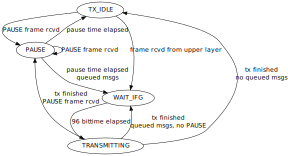
\includegraphics{figures/EtherMACFullDuplex_txstates}
\end{center}

The \nedtype{EtherMACFullDuplex} module records two scalars in addition to the
ones mentioned earlier:
\begin{itemize}
\item \ttt{rx channel idle (\%)}: reception channel idle time
        as a percentage of the total simulation time
\item \ttt{rx channel utilization (\%)}: total reception
        time as a percentage of the total simulation time
\end{itemize}

\subsection{EtherMAC}

Ethernet MAC layer implementing CSMA/CD. It supports both half-duplex and full-duplex operations;
in full-duplex mode it behaves as \nedtype{EtherMACFullDuplex}. In half-duplex  mode
it detects collisions, sends jam messages and retransmit frames upon collisions using
the exponential backoff algorithm. In Gigabit Ethernet networks it supports carrier
extension and frame bursting. Carrier extension can be turned off by setting the
\fpar{carrierExtension} parameter to \ttt{false}.

Unlike \nedtype{EtherMACFullDuplex}, this MAC module processes the incoming packets when their
first bit is received. The end of the reception is calculated by the MAC and
detected by scheduling a self message.

When frames collide the transmission is aborted -- in this case the transmitting
station transmits a jam signal. Jam signals are represented
by a \msgtype{EtherJam} message. The jam message contains the tree identifier
of the frame whose transmission is aborted. When the \nedtype{EtherMAC} receives a jam
signal, it knows that the corresponding transmission ended in jamming and have
been aborted. Thus when it receives as many jams as collided frames, it can
be sure that the channel is free again. (Receiving a jam message marks the
beginning of the jam signal, so actually has to wait for the duration of the jamming.)

The operation of the MAC module can be schematized by the following state chart:

\begin{center}
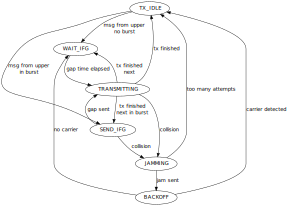
\includegraphics{figures/EtherMAC_txstates}
\end{center}

The module generates these extra signals:
\begin{itemize}
\item \fsignal{collision} when collision starts (received a frame,
         while transmitting or receiving another one; or start to transmit while receiving a frame),
         the constant value 1
\item \fsignal{backoff} when jamming period ended and before waiting according to the
         exponential backoff algorith, the constant value 1
\end{itemize}

These scalar statistics are generated about the state of the line:
\begin{itemize}
  \item \ttt{rx channel idle (\%)} reception channel idle time (full duplex) or channel
         idle time (half-duplex), as a percentage of the total simulation time
  \item \ttt{rx channel utilization (\%)} total successful reception time (full-duplex) or total
         successful reception/transmission time (half duplex), as a percentage
         of the total simulation time
  \item \ttt{rx channel collision (\%)} total unsuccessful reception time, as a percentage
         of the total simulation time
  \item \ttt{collisions} total number collisions (same as count of \fsignal{collisionSignal})
  \item \ttt{backoffs} total number of backoffs (same as count of \fsignal{backoffSignal})
\end{itemize}

% document error conditions (causing error() calls in the code)

% FIXME handleRestransmission() comment is not true: // no beginSendFrames(), because end of jam signal sending will trigger it automatically
%       in case of inner queue, the queued msg is not transmitted
% FIXME should not enter PAUSE state when !duplexMode


\section{Switches}

Ethernet switches play an important role in modern Ethernet LANs. Unlike
passive hubs and repeaters, that work in the physical layer, the switches
operate in the data link layer and routes data frames between the connected
subnets.

While a hub repeats the data frames on each connected line, possibly causing
collisions, switches help to segment the network to small collision domains.
In modern Gigabit LANs each node is connected to the switch direclty
by full-duplex lines, so no collisions are possible. In this case the
CSMA/CD is not needed and the channel utilization can be high.

\subsection{MAC relay units}

INET framework ethernet switches are built from \nedtype{IMACRelayUnit}
components. Each relay unit has N input and output gates for sending/receiving
Ethernet frames. They should be connected to \nedtype{IEtherMAC} modules.

Internally the relay unit holds a table for the destination address -> output
port mapping. When it receives a data frame it updates the table with the
source address->input port. The table can also be pre-loaded from a text file
while initializing the relay unit. The file name given as the \fpar{addressTableFile}
parameter. Each line of the file contains a hexadecimal MAC address and a decimal port
number separated by tabs. Comment lines beginning with '\#' are also allowed:

\begin{verbatim}
01 ff ff ff ff    0
00-ff-ff-ee-d1    1
0A:AA:BC:DE:FF    2
\end{verbatim}

% FIXME #352 addressTableSize is not checked in readAddressTable -> if overflown
%            then later check updateTableWithAddress has no effect
% FIXME format is wrong in the comment of readAddressTable()

The size of the lookup table is restricted by the \fpar{addressTableSize} parameter.
When the table is full, the oldest address is deleted. Entries are also deleted
if their age exceeds the duration given as the \fpar{agingTime} parameter.

If the destination address is not found in the table, the frame is broadcasted.
The frame is not sent to the same subnet it was received from, because the
target already received the original frame. The only exception if the frame
arrived through a radio channel, in this case the target can be out of range.
The port range 0..\fpar{numWirelessPorts}-1 are reserved for wireless connections.

The \nedtype{IMACRelayUnit} module is not a concrete implementation,
it just defines gates and parameters an \nedtype{IMACRelayUnit} should have.
Concrete inplementations add
capacity and performance aspects to the model (number of frames processed
per second, amount of memory available in the switch, etc.)
C++ implementations can subclass from the class \cppclass{MACRelayUnitBase}.

There are two versions of \nedtype{IMACRelayUnit}:

\begin{description}
  \item[\nedtype{MACRelayUnitNP}] models one or more CPUs with shared memory,
    working from a single shared queue.
  \item[\nedtype{MACRelayUnitPP}] models one CPU assigned to each incoming port,
    working with shared memory but separate queues.
\end{description}

In both models input messages are queued. CPUs poll messages from the queue
and process them in \fpar{processingTime}. If the memory usage exceeds
\fpar{bufferSize}, the frame will be dropped.

A simple scheme for sending PAUSE frames is built in (although
users will probably change it). When the buffer level goes
above a high watermark, PAUSE frames are sent on all ports.
The watermark and the pause time is configurable; use zero
values to disable the PAUSE feature.

% FIXME valid values for pauseTime: 0..0xFFFF
% FIXME ETHER_PAUSE_COMMAND_BYTES should be 4 in Ethernet.h (2bytes opcode + 2bytes pauseTime)
% FIXME PAUSE frame should not be sent on all ports probably
% TODO add lowWatermark, send PauseFrame(pauseUnits=0) to resume sending

The relay units collects the following statistics:

\begin{description}
\item[usedBufferBytes] memory usage as function of time
\item[processedBytes] count and length of processed frames
\item[droppedBytes] count and length of frames dropped caused by out of memory
\end{description}

% FIXME MACRelayUnitNP: no signals are generated, how does @statistic work in the ned file?

\subsection{EtherSwitch}

Model of an Ethernet switch containing a relay unit and multiple MAC units.

The duplexChannel attributes of the MACs must be set according to the
medium connected to the port; if collisions are possible (it's a bus or hub)
it must be set to false, otherwise it can be set to true.
By default it uses half duples MAC with CSMA/CD.

\begin{note}
Switches don't implement the Spanning Tree Protocol. You need to
avoid cycles in the LAN topology.
\end{note}

\section{Link Layer Control}
\label{sec:LLC}
% FIXME #353 there is no module for sending EtherFrameWithSNAP frames
% FIXME ETHER_SNAP_HEADER_LENGTH is wrong in Ethernet.h (+3 bytes, ssap+dsap+control)

\subsection{Frame types}

The raw 802.3 frame format header contains the MAC addresses of the destination and source
of the packet and the length of the data field. The frame footer contains the FCS
(Frame Check Sequence) field which is a 32-bit CRC.

\begin{center}
\begin{bytefield}[bitwidth=1.2em,bitheight=2\baselineskip]{20}
\bitbox{4}{\small MAC \\ destination} &
\bitbox{4}{\small MAC \\ source} &
\bitbox{4}{\small Length} &
\bitbox{4}{\small Payload} &
\bitbox{4}{\small FCS} \\
\bitbox{4}{\small 6 octets} &
\bitbox{4}{\small 6 octets} &
\bitbox{4}{\small 2 octets} &
\bitbox{4}{\small 46-1500 octets} &
\bitbox{4}{\small 4 octets}
\end{bytefield}
\end{center}

Each such frame is preceded by a 7 octet Preamble (with 10101010 octets) and
a 1 octet SFD (Start of Frame Delimiter) field (10101011) and followed by an
12 octet interframe gap. These fields are added and removed in the MAC layer,
so they are omitted here.

When multiple upper layer protocols use the same Ethernet line,
the kernel has to know which which component handles the incoming frames.
For this purpose a protocol identifier was added to the standard Ethernet
frames.

The first solution preceded the 802.3 standard and used a 2 byte protocol
identifier in place of the Length field. This is called Ethernet II
or DIX frame.
Each protocol id is above 1536, so the Ethernet II frames and the 802.3
frames can be distinguished.

\begin{center}
\begin{bytefield}[bitwidth=1.2em,bitheight=2\baselineskip]{20}
\bitbox{4}{\small MAC \\ destination} &
\bitbox{4}{\small MAC \\ source} &
\bitbox{4}{\small EtherType} &
\bitbox{4}{\small Payload} &
\bitbox{4}{\small FCS} \\
\bitbox{4}{\small 6 octets} &
\bitbox{4}{\small 6 octets} &
\bitbox{4}{\small 2 octets} &
\bitbox{4}{\small 46-1500 octets} &
\bitbox{4}{\small 4 octets}
\end{bytefield}
\end{center}

The LLC frame format uses a 1 byte source, a 1 byte destination, and a 1 byte
control information to identify the encapsulated protocol adopted from the
802.2 standard. These fields follow the standard 802.3 header, so the maximum
length of the payload is 1497 bytes:

\begin{center}
\begin{bytefield}[bitwidth=1.2em,bitheight=2\baselineskip]{20}
\bitbox{4}{\small MAC \\ destination} &
\bitbox{4}{\small MAC \\ source} &
\bitbox{4}{\small Length} &
\bitbox{4}{\small DSAP} &
\bitbox{4}{\small SSAP} &
\bitbox{4}{\small Control} &
\bitbox{4}{\small Payload} &
\bitbox{4}{\small FCS} \\
\bitbox{4}{\small 6 octets} &
\bitbox{4}{\small 6 octets} &
\bitbox{4}{\small 2 octets} &
\bitbox{4}{\small 1 octets} &
\bitbox{4}{\small 1 octets} &
\bitbox{4}{\small 1 octets} &
\bitbox{4}{\small 43-1497 octets} &
\bitbox{4}{\small 4 octets}
\end{bytefield}
\end{center}

The SNAP header uses the EtherType protocol identifiers inside an LLC header.
The SSAP and DSAP fields are filled with 0xAA (SAP\_SNAP), and the control
field is 0x03. They are followed by a 3 byte orgnaization and a 2 byte local
code the identify the protocol. If the organization code is 0, the local field
contains an EtherType protocol identifier.

\begin{center}
\begin{bytefield}[bitwidth=1.2em,bitheight=2\baselineskip]{20}
\bitbox{4}{\small MAC \\ destination} &
\bitbox{4}{\small MAC \\ source} &
\bitbox{4}{\small Length} &
\bitbox{4}{\small DSAP \\ 0xAA} &
\bitbox{4}{\small SSAP \\ 0xAA} &
\bitbox{4}{\small Control \\ 0x03} &
\bitbox{4}{\small OrgCode} &
\bitbox{4}{\small Local \\ Code} &
\bitbox{4}{\small Payload} &
\bitbox{4}{\small FCS} \\
\bitbox{4}{\small 6 octets} &
\bitbox{4}{\small 6 octets} &
\bitbox{4}{\small 2 octets} &
\bitbox{4}{\small 1 octets} &
\bitbox{4}{\small 1 octets} &
\bitbox{4}{\small 1 octets} &
\bitbox{4}{\small 3 octets} &
\bitbox{4}{\small 2 octets} &
\bitbox{4}{\small 38-1492 octets} &
\bitbox{4}{\small 4 octets}
\end{bytefield}
\end{center}

The INET defines these frames in the \ffilename{EtherFrame.msg} file.
The models supports Ethernet II, 803.2 with LLC header, and 803.3 with LLC and SNAP headers.
The corresponding classes are:
\msgtype{EthernetIIFrame}, \msgtype{EtherFrameWithLLC} and \msgtype{EtherFrameWithSNAP}. They all class
from \msgtype{EtherFrame} which only represents the basic MAC frame with source and
destination addresses. \nedtype{EtherMAC} only deals with \msgtype{EtherFrame}s, and does not
care about the specific subclass.

Ethernet frames carry data packets as encapsulated cMessage objects.
Data packets can be of any message type (cMessage or cMessage subclass).

The model encapsulates data packets in Ethernet frames using the \ttt{encapsulate()}
method of cMessage. Encapsulate() updates the length of the Ethernet frame too,
so the model doesn't have to take care of that.

The fields of the Ethernet header are passed in a \cppclass{Ieee802Ctrl}
control structure to the LLC by the network layer.


EtherJam, EtherPadding (interframe gap), EtherPauseFrame?


\subsection{EtherEncap}

The \nedtype{EtherEncap} module generates \msgtype{EthernetIIFrame} messages.

EtherFrameII

\subsection{EtherLLC}

EtherFrameWithLLC

SAP registration

% TODO delete EtherLLC, because LLC without SNAP is not used with IP (no ARP,IPv6 SAP)
% TODO modify EtherEncap to handle EtherFrameWithSNAP frames too (we can not send EtherFrameWithSNAP now)

\subsubsection{\nedtype{EtherLLC} and higher layers}

The \nedtype{EtherLLC} module can serve several applications (higher layer protocols),
and dispatch data to them. Higher layers are identified by DSAP.
See section "Application registration" for more info.

\nedtype{EtherEncap} doesn't have the functionality to dispatch to different
higher layers because in practice it'll always be used with IP.

\subsubsection{Communication between LLC and Higher Layers}

Higher layers (applications or protocols) talk to the \nedtype{EtherLLC} module.

When a higher layer wants to send a packet via Ethernet, it just
passes the data packet (a cMessage or any subclass) to \nedtype{EtherLLC}.
The message kind has to be set to IEEE802CTRL\_DATA.

In general, if \nedtype{EtherLLC} receives a packet from the higher layers,
it interprets the message kind as a command. The commands include
IEEE802CTRL\_DATA (send a frame), IEEE802CTRL\_REGISTER\_DSAP (register highher layer)
IEEE802CTRL\_DEREGISTER\_DSAP (deregister higher layer) and IEEE802CTRL\_SENDPAUSE
(send PAUSE frame) -- see EtherLLC for a more complete list.

The arguments to the command are NOT inside the data packet but
in a "control info" data structure of class \cppclass{Ieee802Ctrl}, attached to
the packet. See controlInfo() method of cMessage (OMNeT++ 3.0).

For example, to send a packet to a given MAC address and protocol
identifier, the application sets the data packet's message kind
to ETH\_DATA ("please send this data packet" command),
fills in the \nedtype{Ieee802Ctrl} structure with the destination MAC address and
the protocol identifier, adds the control info to the message, then sends
the packet to \nedtype{EtherLLC}.

When the command doesn't involve a data packet (e.g.
IEEE802CTRL\_(DE)REGISTER\_DSAP, IEEE802CTRL\_SENDPAUSE), a dummy packet
(empty cMessage) is used.

\subsubsection{Rationale}

The alternative of the above communications would be:

\begin{itemize}
  \item adding the parameters such as destination address into the data
    packet. This would be a poor solution since it would make the
    higher layers specific to the Ethernet model.
  \item encapsulating a data packet into an \textit{interface packet} which
    contains the destination address and other parameters. The
    disadvantages of this approach is the overhead associated with
    creating and destroying the interface packets.
\end{itemize}

Using a control structure is more efficient than the interface packet
approach, because the control structure can be created once inside
the higher layer and be reused for every packet.

It may also appear to be more intuitive in Tkenv because one can observe
data packets travelling between the higher layer and Ethernet
modules -- as opposed to "interface" packets.


\subsubsection{EtherLLC: SAP Registration}

The Ethernet model supports multiple applications or higher layer
protocols.

So that data arriving from the network can be dispatched to the
correct applications (higher layer protocols), applications
have to register themselves in \nedtype{EtherLLC}. The registration
is done with the IEEE802CTRL\_REGISTER\_DSAP command
(see section "Communication between LLC and higher layers")
which associates a SAP with the LLC port. Different applications
have to connect to different ports of \nedtype{EtherLLC}.

The ETHERCTRL\_REGISTER\_DSAP/IEEE802CTRL\_DEREGISTER\_DSAP commands use only the
dsap field in the \cppclass{Ieee802Ctrl} structure.

\subsection{EthernetInterface module}

The \nedtype{EthernetInterface} compound module implements the \nedtype{IWiredNic}
interface. Complements \nedtype{EtherMAC} and \nedtype{EtherEncap} with an output queue
for QoS and RED support. It also has configurable input/output filters as \nedtype{IHook}
components similarly to the \nedtype{PPPInterface} module.

% TODO there is no IWiredNic with EtherLLC

\section{Ethernet applications}

The \nedtype{inet.applications.ethernet} package contains modules
for a simple client-server application. The \nedtype{EtherAppCli} is a simple
traffic generator that peridically sends \msgtype{EtherAppReq} messages
whose length can be configured. destAddress, startTime,waitType, reqLength, respLength

The server component of the model (\nedtype{EtherAppSrv}) responds with a
\msgtype{EtherAppResp} message of the requested length. If the response does
not fit into one ethernet frame, the client receives the data in multiple
chunks.

% FIXME reqLength>1500 causes an error in the LLC module
% FIXME numFrames field of EtherAppRes is not used
% FIXME server always sends 1497 byte chunks, it should depend on the framing (1497 is for LLC)
% FIXME if registerSAP is false (default), the and EtherLLC used, then the client won't receive messages (auto config?)
% FIXME Ieee802Nic -> EthernetInterface in the NED comment

Both applications have a \fpar{registerSAP} boolean parameter.
This parameter should be set to \ttt{true} if the application is connected
to the \nedtype{EtherLLC} module which requires registration of the SAP
before sending frames.

Both applications collects the following statistics: sentPkBytes, rcvdPkBytes,
endToEndDelay.

The client and server application works with any model that accepts
Ieee802Ctrl control info on the packets (e.g. the 802.11 model).
The applications should be connected directly to the \nedtype{EtherLLC}
or an EthernetInterface NIC module.

The model also contains a host component that groups the applications
and the LLC and MAC components together (\nedtype{EtherHost}). This node does
not contain higher layer protocols, it generates Ethernet traffic directly.
By default it is configured to use half duplex MAC (CSMA/CD).

\section{Ethernet networks}

\subsection{\nedtype{LargeNet} model}

The \nedtype{LargeNet} model demonstrates how one can put together models of large
LANs with little effort, making use of MAC auto-configuration.

\nedtype{LargeNet} models a large Ethernet campus backbone. As configured in the
default omnetpp.ini, it contains altogether about 8000 computers
and 900 switches and hubs. This results in about 165MB process size
on my (32-bit) linux box when I run the simulation.
The model mixes all kinds of Ethernet technology: Gigabit Ethernet,
100Mb full duplex, 100Mb half duplex, 10Mb UTP, 10Mb bus ("thin Ethernet"),
switched hubs, repeating hubs.

The topology is in \nedtype{LargeNet}.ned, and it looks like this: there's chain
of n=15 large "backbone" switches (switchBB[]) as well as four more
large switches (switchA, switchB, switchC, switchD) connected to
somewhere the middle of the backbone (switchBB[4]). These 15+4 switches
make up the backbone; the n=15 number is configurable in omnetpp.ini.

Then there're several smaller LANs hanging off each backbone switch.
There're three types of LANs: small, medium and large (represented by
compound module types \nedtype{SmallLAN}, \nedtype{MediumLAN}, \nedtype{LargeLAN}). A small LAN
consists of a few computers on a hub (100Mb half duplex); a medium
LAN consists of a smaller switch with a hub on one of its port
(and computers on both); the large one also has a switch and a hub,
plus an Ethernet bus hanging of one port of the hub (there's still hubs
around with one BNC connector besides the UTP ones).
By default there're 5..15 LANs of each type hanging off each backbone
switch. (These numbers are also omnetpp.ini parameters like the length
of the backbone.)

The application model which generates load on the simulated LAN is
simple yet powerful. It can be used as a rough model for any
request-response based protocol such as SMB/CIFS (the Windows file
sharing protocol), HTTP, or a database client-server protocol.

Every computer runs a client application (\nedtype{EtherAppCli}) which connects
to one of the servers. There's one server attached to switches A, B,
C and D each: serverA, serverB, serverC and serverD -- server selection
is configured in omnetpp.ini). The servers run \nedtype{EtherAppSrv}.
Clients periodically send a request to the server, and the request
packet contains how many bytes the client wants the server to send back
(this can mean one or more Ethernet frames, depending on the byte count).
 Currently the request and reply lengths are configured in omnetpp.ini
as intuniform(50,1400) and truncnormal(5000,5000).

The volume of the traffic can most easily be controlled with the
time period between sending requests; this is currently
set in omnetpp.ini to exponential(0.50) (that is, average 2
requests per second). This already causes frames to be dropped
in some of the backbone switches, so the network is a bit
overloaded with the current settings.

The model generates extensive statistics. All MACs (and most other
modules too) write statistics into omnetpp.sca at the end
of the simulation: number of frames sent, received, dropped, etc.
These are only basic statistics, however it still makes the
scalar file to be several ten megabytes in size. You can use
the analysis tools provided with OMNeT++ to visualized the data
in this file. (If the file size is too big, writing statistics
can be disabled, by putting **.record-scalar=false in the ini file.)
The model can also record output vectors, but this is currently
disabled in omnetpp.ini because the generated file can easily reach
gigabyte sizes.

%%% Local Variables:
%%% mode: latex
%%% TeX-master: "usman"
%%% End:

\cleardoublepage

\chapter{The 802.11 Model}
\label{cha:80211}

% https://summit.omnetpp.org/archive/2016/assets/pdf/OMNET-2016-Session_9-02-Presentation.pdf

\section{Overview}

This chapter provides an overview of the IEEE 802.11 model for the INET Framework.

An IEEE 802.11 interface (NIC) comes in several flavours, differring
in their role (ad-hoc station, infrastructure mode station, or
access point) and their level of detail:

\begin{enumerate}
 \item \nedtype{Ieee80211Interface}: a generic (configurable) NIC
 \item \nedtype{Ieee80211NicAdhoc}: for ad-hoc mode
 \item \nedtype{Ieee80211NicAP}, \nedtype{Ieee80211NicAPSimplified}: for use in an access point
 \item \nedtype{Ieee80211NicSTA}, \nedtype{Ieee80211NicSTASimplified}: for use in an
   infrastructure-mode station
\end{enumerate}

NICs consist of four layers, which are the following (in top-down order):

\begin{enumerate}
  \item agent
  \item management
  \item MAC
  \item physical layer (radio)
\end{enumerate}

The following sections examine the above components.

\section{MAC}

The \nedtype{Ieee80211Mac} module type represents the IEEE 802.11 MAC.
The implementation is entirely based on the standard IEEE 802.11™-2012 Part 11:
Wireless LAN Medium Access Control (MAC) and Physical Layer (PHY)
Specifications.

\nedtype{Ieee80211Mac} performs transmission of frames according
to the CSMA/CA protocol. It receives data and management frames from
the upper layers, and transmits them.

The \nedtype{Ieee80211Mac} was designed to be modular to facilitate experimenting
with new policies, features and algorithms within the MAC layer. Users can
easily replace individual components with their own implementations. Policies,
which most likely to be experimented with, are extracted into their own modules.

The model has the following replaceable built-in policies:

\begin{itemize}
  \item ACK policy
  \item RTS/CTS policy
  \item Originator and recipient block ACK agreement policies
  \item MSDU aggregation policy
  \item Fragmentation policy
\end{itemize}

The new model also separates the following components:

\begin{itemize}
  \item Coordination functions
  \item Channel access methods
  \item MAC data services
  \item Aggregation and deaggregation
  \item Fragmentation and defragmentation
  \item Block ACK agreements and reordering
  \item Frame exchange sequences
  \item Duplicate removal
  \item Rate selection
  \item Rate control
  \item Protection mechanisms
  \item Recovery procedure
  \item Contention
  \item Frame queues
  \item TX/RX
\end{itemize}

\section{Physical Layer}

\textit{The physical layer} modules (\nedtype{Ieee80211Radio}) deal with modelling
transmission and reception of frames. They model the characteristics of
the radio channel, and determine if a frame was received correctly
(that is, it did not suffer bit errors due to low signal power or
interference in the radio channel). Frames received correctly are passed
up to the MAC. The implementation of these modules is based on the
Mobility Framework.

\section{Management}

\textit{The management layer} performs encapsulation and decapsulation of data packets
for the MAC, and exchanges management frames via the MAC with its peer
management entities in other STAs and APs. Beacon, Probe Request/Response,
Authentication, Association Request/Response etc frames are generated
and interpreted by management entities, and transmitted/received via
the MAC layer. During scanning, it is the management entity that periodically
switches channels, and collects information from received beacons and
probe responses.

The management layer has several implementations which differ in their role
(STA/AP/ad-hoc) and level of detail: \nedtype{Ieee80211MgmtAdhoc},
\nedtype{Ieee80211MgmtAp}, \nedtype{Ieee80211MgmtApSimplified}, \nedtype{Ieee80211MgmtSta},
\nedtype{Ieee80211MgmtStaSimplified}. The ..Simplified ones differ from the others
in that they do not model the scan-authenticate-associate process,
so they cannot be used in experiments involving handover.

\section{Agent}

The agent is what instructs the management layer to perform
scanning, authentication and association. The management layer itself
just carries out these commands by performing the scanning, authentication
and association procedures, and reports back the results to the agent.

The agent layer is currenly only present in the \nedtype{Ieee80211NicSTA} NIC module,
as an \nedtype{Ieee80211AgentSta} module. The managament entities in other NIC
variants do not have as much freedom as to need an agent to control them.

By modifying or replacing the agent, one can alter the dynamic behaviour
of STAs in the network, for example implement different handover strategies.


%%% Local Variables:
%%% mode: latex
%%% TeX-master: "usman"
%%% End:


\cleardoublepage

\chapter{The 802.15.4 Model}
\label{cha:802154}

\section{Overview}
\label{sec:802154:overview}

IEEE 802.15.4 is a technical standard which defines the operation of low-rate
wireless personal area networks (LR-WPANs). IEEE 802.15.4 was designed for data
rates of 250 kbit/s or lower, in order to achieve long battery life (months or
even years) and very low complexity. The standard specifies the physical layer
and media access control.

IEEE 802.15.4 is the basis for the ZigBee, ISA100.11a, WirelessHART, MiWi, SNAP,
and the Thread specifications, each of which further extends the standard by
developing the upper layers which are not defined in IEEE 802.15.4.
Alternatively, it can be used with 6LoWPAN, the technology used to deliver IPv6
over WPANs, to define the upper layers. (Thread is also 6LoWPAN-based.)

The INET Framework contains a basic implementation of IEEE 802.15.4 protocol.


\section{Network Interfaces}
\label{sec:802154:network-interfaces}

There are two network interfaces that differ in the type of radio:

\begin{itemize}
  \item \nedtype{Ieee802154NarrowbandInterface} is for use with narrowband radios
  \item \nedtype{Ieee802154UwbIrInterface} is for use with the UWB-IR radio
\end{itemize}


To create a wireless node with a 802.15.4 interface, use a node type
that has a wireless interface, and set the interface type to the
appropriate type. For example, \nedtype{WirelessHost} is a node type
which is preconfigured to have one wireless interface, \ttt{wlan[0]}.
\ttt{wlan[0]} is of parametric type, so if you build the network from
\nedtype{WirelessHost} nodes, you can configure all of them to use
802.15.4 with the following line in the ini file:

\begin{inifile}
**.wlan[0].typename = "Ieee802154NarrowbandInterface"
\end{inifile}

\section{Physical Layer}
\label{sec:802154:physical-layer}

The IEEE 802.15.4 standard defines several alternative PHYs. There are
several narrowband radios at various frequency bands using various modulation
schemes (DSSS, O-QPSK, MPSK, GFSK BPSK, etc.), a Direct Sequence ultra-wideband
(UWB), and one using chirp spread spectrum (CSS).

INET provides the following radios:

\begin{itemize}
  \item \nedtype{Ieee802154NarrowbandScalarRadio} is currently a partially
    parameterized version of the APSK radio. Before using this radio,
    one must check its parameters and make sure that they correspond to the
    specification of the 802.15.4 narrowband PHY to be simulated.
  \item \nedtype{Ieee802154UwbIrRadio} models the 802.14.5 UWB radio.
\end{itemize}

One must choose a matching medium model, for example
\nedtype{Ieee802154UwbIrRadioMedium} for \nedtype{Ieee802154UwbIrRadio},
and \nedtype{Ieee802154NarrowbandScalarRadioMedium} for
\nedtype{Ieee802154\-NarrowbandScalarRadio}.


\section{MAC Protocol}
\label{sec:802154:mac-protocol}

The 802.15.4 MAC is based on collision avoidance via CSMA/CA. Important other
features include real-time suitability by reservation of guaranteed time slots,
and integrated support for secure communications. Devices also include power
management functions such as link quality and energy detection.

The \nedtype{Ieee802154Mac} type in INET is currently a parameterized
version of a generic CSMA/CA protocol model with ACK support.

There is also a \nedtype{Ieee802154NarrowbandMac}.


%%% Local Variables:
%%% mode: latex
%%% TeX-master: "usman"
%%% End:


\cleardoublepage

\chapter{MAC Protocols for Wireless Sensor Networks}
\label{cha:sensor-macs}

\section{Overview}
\label{sec:sensor-macs:overview}

The INET Framework contains the implementation of several MAC protocols
for wireless sensor networks (WSNs), including B-MAC, L-MAC and X-MAC.

To create a wireless node with a specific MAC protocol, use a node type
that has a wireless interface, and set the interface type to the
appropriate type. For example, \nedtype{WirelessHost} is a node type
which is preconfigured to have one wireless interface, \ttt{wlan[0]}.
\ttt{wlan[0]} is of parametric type, so if you build the network from
\nedtype{WirelessHost} nodes, you can configure all of them to use
e.g. B-MAC with the following line in the ini file:

\begin{inifile}
**.wlan[0].typename = "BMacInterface"
\end{inifile}


\section{B-MAC}
\label{sec:sensor-macs:b-mac}

B-MAC (Berkeley MAC) is a carrier sense media access protocol for
wireless sensor networks that provides a flexible interface to obtain
ultra low power operation, effective collision avoidance, and
high channel utilization. To achieve low power operation,
B-MAC employs an adaptive preamble sampling scheme to reduce duty cycle
and minimize idle listening. B-MAC is designed for low traffic,
low power communication, and is one of the most widely used
protocols (e.g. it is part of TinyOS).

The \nedtype{BMac} module type implements the B-MAC protocol.

\nedtype{BMacInterface} is a \nedtype{WirelessInterface} with the MAC type
set to \nedtype{BMac}.


\section{L-MAC}
\label{sec:sensor-macs:l-mac}

L-MAC (Lightweight MAC) is an energy-efficient medium acces protocol designed
for wireless sensor networks. Although the protocol uses TDMA to give nodes
in the WSN the opportunity to communicate collision-free, the network is
self-organizing in terms of time slot assignment and synchronization.
The protocol reduces the number of transceiver state switches and hence
the energy wasted in preamble transmissions.

The \nedtype{LMac} module type implements the L-MAC protocol, based on the
paper ``A lightweight medium access protocol (LMAC) for wireless sensor networks''
by van Hoesel and P. Havinga.

\nedtype{LMacInterface} is a \nedtype{WirelessInterface} with the MAC type
set to \nedtype{LMac}.


\section{X-MAC}
\label{sec:sensor-macs:x-mac}

X-MAC is a low-power MAC protocol for wireless sensor networks (WSNs).
In contrast to B-MAC which employs an extended preamble and preamble sampling,
X-MAC uses a shortened preamble that reduces latency at each hop and
improves energy consumption while retaining the advantages
of low power listening, namely low power communication, simplicity
and a decoupling of transmitter and receiver sleep schedules.

The \nedtype{XMac} module type implements the X-MAC protocol, based on
the paper ``X-MAC: A Short Preamble MAC Protocol for Duty-Cycled
Wireless Sensor Networks'' by Michael Buettner, Gary V. Yee, Eric Anderson
and Richard Han.

\nedtype{XMacInterface} is a \nedtype{WirelessInterface} with the MAC type
set to \nedtype{XMac}.


%%% Local Variables:
%%% mode: latex
%%% TeX-master: "usman"
%%% End:


\cleardoublepage

\ifdraft TODO

\chapter{The Physical Layer}
\label{cha:physicallayer}

TODO which modules? C++ interface

\begin{itemize}
  \item ongoing transmissions
  \item recent successful receptions
  \item recent obstacle intersections and surface normal vectors
\end{itemize}

\begin{verbatim}
TODO: 
 - exploit multiple CPUs and the highly parallel GPU to increase performance
 - provide performance vs. accuracy tradeoff configuration options
   (e.g. range filter, radio mode filter, listening mode filter, MAC address filter)
 - support different level of details (see details below)
 - support different transmitters and receivers (scale from flat to layered models)
 - support different radio signal models (scale from range based to accurate emulation models)
 - support different propagation models (scale from immediate to accurate models)
 - support different attenuation models (scale from free space to trace based models)
 - support different antenna models (scale from isotropic to directional models)
 - support different power consumption models (scale from mode based to signal based models)
 - provide concurrent transmitter and receiver mode (transceiver mode)
 - provide burst mode (back to back) transmissions
 - provide synchronization/preamble detection
 - provide capture during reception (switching to another transmission)
 - provide finite time radio mode switching

TODO: scalar vs dimensional
TODO: flat vs layered
TODO: Generic, IEEE 802.11, IEEE 802.15.4
TODO: acoustic underwater example
TODO: wireless vs. wired medium

\end{verbatim}

\section{Overview}

Today's electric devices use more and more wireless communication methods such
as Wifi, Bluetooth, NFC, UMTS, and LTE. Despite the diversity of these devices
there are many similarities in the modeling of their physical layer components.
The models often have similar signal representations and signal processing steps,
and they also share the physical medium model where communication takes place.

In general, the physical layer simulation is a very time consuming task. The
simulation of signal propagation, signal fading, signal interference, and signal
decoding in detail may often result in unacceptable performance. Finding the
right abstractions, the right level of detail, and the right trade-offs between
accuracy and performance is difficult and very important.

To summarize, the physical layer is designed with the following goals in mind:
\begin{itemize}
  \item customizability
  \item extensibility
  \item scalable level of detail
  \item ability to exploit parallel hardware
\end{itemize}

The following sections provide a brief overview of the physical layer model. For
more details on the available modules, their parameterization and the actual
implementations please refer to the documentation in the corresponding NED and
C++ source files.

\subsection{Customizability}

Real world communication devices often provide a wide variety of configuration
options to allow adapting to the physical conditions where they are required
to operate. For example, a Wifi router administration interface often provides
parameters to configure the transmission power, bitrate, preamble type, carrier
frequency, RTS threshold, beacon interval, etc. Mostly these parameters have
default values assigned, so the user doesn't have to set them separately, but
may override them as needed.

Similarly to real world devices the physical layer models also provide a wide
variety of parameters to control their behavior. The most common NED parameters
are various physical quantities with physical units such as transmission power
\ttt{[W]}, reception sensitivity \ttt{[W]}, carrier frequency \ttt{[Hz]},
communication range \ttt{[m]}, propagation speed \ttt{[m/s]}, SNIR reception
threshold \ttt{[dB]}, bitrate \ttt{[b/s]}. Occasionally models support new
parameters or new combinations, which don't exist in real world hardware, to
allow further experimentation.

Another important and commonly used parameter kind selects among alternative
implementations of a particular interface by providing its name. Different
implementations are often separate modules, which come with their own set of
parameters to avoid the confusion of mixing their unrelated parameters. Some
modules may be split into more submodules. This further deepens the module
hierarchy, but allows better extensibility.

\subsection{Extensibility}

Similarly to designing other simulation models, modeling the physical layer is
not at all an unambiguous task. For example, the research literature contains a
number of different path loss models for signal propagation, there are different
bit error models for a particular protocol standard, representing the signal in
the analog domain can also be done in several different ways, and so on.

In order to support this diversity the physical layer is designed to be
extensible with alternative implementations at various parts of the model. This
is realized by separately defining C++ and NED interfaces between modules, and
also by providing parameters in their parent modules to easily select among the
available implementations.

New models can be added by implementing the required interfaces from scratch, or
by deriving from already existing implementations and overriding functionality.
This architecture allows the user to create new models with less effort, and to
focus on the real differences, while the rest of the physical layer remains the
same.

\subsection{Scalable Level of Detail}

There are many possible ways to model various aspects of the physical layer.
The most important difference lies in the trade-off between performance versus
accuracy. In order to support the different trade-offs the physical layer is
designed to be scalable with respect to the simulated level of detail. In other
words, it's scalable from high-performance less accurate simulations to high
fidelity slower simulations.

The physical layer model is scalable along the following axes:

\begin{itemize}
  \item simulation model -- statistical vs accurate
  \item software architecture -- flat vs layered
  \item data representation -- scalar vs multi-dimensional
  \item number of messages -- TODO 
\end{itemize}

The simulation model might vary from simple statistical models to accurate
emulation. The simplest models ignore the actual bits of the transmission. For
example, the extremely simple unit disc radio even ignores the signal power. The
most accurate models use precise signal representation for all four domains:
bit domain, symbol domain, sample domain, and analog domain representations.
They also emulate most functions of real hardware in detail: forward error
correction, interleaving, scrambling, modulation, spreading, pulse shaping, and
so on.

The software architecture might vary from flat to layered. A flat architecture
is efficient but not modular. Functionality can only be affected through simple
parameters and not by providing alternative implementations. Whereas a layered
architecture is more flexible at the cost of more complex data structures, more
data conversions, more resource management, and thus slower processing. On the
other hand, it provides more customization opportunities to replace parts with
alternative implementations and to do research easier in the area.

The data representation might vary from scalar to multidimensional values. In
the analog domain of the physical layer data quite often changes over time,
frequency, space, or any combination thereof. The most obvious example is the
analog signal power, but there are others such as signal phase or the signal to
noise ratio.

The number of messages per transmission added to the future event queue might
vary from one to the number of radios. One message might be sufficient, for
example, if the transmission is intended to a single destination, and other
receivers are either not affected, or the effect is negligible. On the other
hand, it might be necessary to process all transmissions by all receivers in
order to have the desired effect on the higher layers. For example, if a MAC
model is configured to promiscuous mode, it needs to receive all transmissions.

\subsection{Exploiting Parallel Hardware}

The physical processes simulated by the physical layer are inherently parallel.
The computation of the transmission arrival space-time coordinates, the analog
signal representation of transmissions and receptions, the interfering
receptions and noises, the signal to noise ratio, the decoded bits, the bit
errors, and the physical layer indications all provide a good parallelization
opportunity, because they dominate the physical layer performance and are
independent for each receiver. Therefore the physical layer is designed to be
able to utilize parallel hardware, multi-core CPUs, vector instructions and the
highly parallel GPU.

The idea is to have a central component in the software architecture where
parallel computation can happen. This central component is the medium model
that knows about all radios, transmissions, interferences, and receptions
anyway. It uses optimistic parallel computation in multiple background threads
while the main simulation thread continues normal execution. When a new
transmission enters the channel the already computed and affected results are
invalidated or updated, and the affected ongoing optimistic parallel
computations are canceled.

\section{The Radio Model}

The radio model describes the physical device that is capable of transmitting
and receiving signals on the medium. It contains an antenna model, a transmitter
model, a receiver model, and an energy consumer model. The antenna model is
shared between the transmitter model and the receiver model. The separation of
the transmitter model and the receiver model allows asymmetric configurations.
The energy consumer model is optional and it's only used when the simulation of
energy consumption is necessary.

The radio model has an operational mode that is called the radio mode. The radio
mode is externally controlled usually by the MAC model. In transceiver mode, the
radio can simultaneously transmit and receive a signal. Changing the radio mode
may optionally take a non-zero amount of time. The supported radio modes are the
following:

\begin{itemize}
  \item \ttt{off}: communication isn't possible, energy consumption is zero
  \item \ttt{sleep}: communication isn't possible, energy consumption is minimal
  \item \ttt{receiver}: only reception is possible, energy consumption is low
  \item \ttt{transmitter}: only transmission is possible, energy consumption is
high
  \item \ttt{transceiver}: reception and transmission is simultaneously
possible, energy consumption is high
  \item \ttt{switching}: communication isn't possible, energy consumption is
minimal
\end{itemize}

In addition to the radio mode, the transmitter and the receiver models have
separate states which describe what they are doing. Changes to these states are
automatically published by the radio. The signaled transmitter states are the
following:

\begin{itemize}
  \item \ttt{undefined}: isn't operating
  \item \ttt{idle}: there's no transmission in progress
  \item \ttt{transmitting}: transmission is in progress
\end{itemize}

The signaled receiver states are the following:

\begin{itemize}
  \item \ttt{undefined}: isn't operating
  \item \ttt{idle}: there's no reception in progress
  \item \ttt{busy}: received signal is not interpretable
  \item \ttt{synchronizing}: synchronization is in progress
  \item \ttt{receiving}: reception is in progress
\end{itemize}

When a radio wants to transmit a signal on the medium it sends direct messages
to all affected radios with the help of the central medium module. The messages
contain a shared data structure which describes the transmission the way it
entered the medium. The messages arrive at the moment when start of the
transmission arrive at the receiver. The receiver radios also handle the
incoming messages with the help of the central medium module. This kind of
centralization allows the medium to do shared computations in a more efficient
way and it also makes parallel computation possible.

As stated above the radio module utilizes multiple submodules to further split
its task. This design decision makes it more extensible and customizable. The
following sections describe the parts of the radio model.

\subsection{Antenna Models}

The antenna model describes the effects of the physical device which converts
electric signals into radio waves, and vice versa. This model captures the
antenna characteristics that heavily affect the quality of the communication
channel. For example, various antenna shapes, antenna size and geometry, antenna
arrays, and antenna orientation causes different directional or frequency
selectivity.

The antenna model provides a position and an orientation using a mobility model
that defaults to the mobility of the node. The main purpose of this model is to
compute the antenna gain based on the specific antenna characteristics and the
direction of the signal. The signal direction is computed by the medium from the
position and the orientation of the transmitter and the receiver. The following
list provides some examples:

\begin{itemize}
  \item \nedtype{IsotropicAntenna}: antenna gain is exactly 1 in any direction
  \item \nedtype{ConstantGainAntenna}: antenna gain is a constant determined by
a parameter
  \item \nedtype{DipoleAntenna}: antenna gain depends on the direction according
to the dipole antenna characteristics
  \item \nedtype{InterpolatingAntenna}: antenna gain is computed by linear
interpolation according to a table indexed by the direction angles
\end{itemize}

The antenna models are in the \ttt{src/physicallayer/antenna/} directory.

\subsection{Transmitter Models}

The transmitter model describes the physical process which converts packets into
electric signals. In other words, this model converts a MAC packet into a signal
that is transmitted on the medium. The conversion process and the representation
of the signal depends on the level of detail and the physical characteristics
of the implemented protocol.

In the flat model the transmitter model skips the symbol domain and the sample
domain representations, and it directly creates the analog domain representation.
The bit domain representation is reduced to the bit length of the packet and the
actual bits are ignored.

In the layered model the conversion process involves various processing steps
such as packet serialization, forward error correction encoding, scrambling,
interleaving, and modulation. This transmitter model requires much more
computation, but it produces accurate bit domain, symbol domain, and sample
domain representations.

The various protocol specific transmitter models are in the corresponding
directories.

\subsection{Receiver Models}

The receiver model describes the physical process which converts electric
signals into packets. In other words, this model converts a reception, along
with an interference computed by the medium model, into a MAC packet and a
reception indication. It also determines the following for each transmission: 

\begin{itemize}
  \item \ttt{is the reception possible or not}: based on the signal
characteristics such as reception power, carrier frequency, bandwidth, preamble
mode, modulation scheme
  \item \ttt{if the reception is possible, is reception attempted or not}: based
on the ongoing reception and the support of signal capturing
  \item \ttt{if the reception is attempted, is reception successful or not}:
based on the error model and the simulated part of the signal decoding
\end{itemize}

In the flat model the receiver model skips the sample domain, the symbol domain,
and the bit domain representations, and it directly creates the packet domain
representation by copying the packet from the transmission. It uses the error
model to decide if the reception is successful or not.

In the layered model the conversion process involves various processing steps
such as demodulation, descrambling, deinterleaving, forward error correction
decoding, and deserialization. This reception model requires much more
computation, but it produces accurate sample domain, symbol domain, and bit
domain representations.

The various protocol specific receiver models are in the corresponding 
directories.

\subsection{Transmission Error Modeling}

Determining the reception errors is a crucial part of the reception process.
There are often several different statistical error models in the literature
even for a particular physical layer. In order to support this diversity the
error model is a separate replaceable component of the receiver. 

The error model describes how the signal to noise ratio affects the amount of
errors at the receiver. The main purpose of this model is to determine whether
if the received packet has errors or not. It also computes various physical
layer indications for higher layers such as packet error rate, bit error rate,
and symbol error rate. For the layered reception model it needs to compute the
erroneous bits, symbols, or samples depending on the lowest simulated physical
domain where the real decoding starts. The error model is optional, if omitted
all receptions are considered successful.

The error models are in the \ttt{src/physicallayer/errormodel/} directory and
also in the corresponding protocol specific directories.

\subsection{Power Consumption Models}

A substantial part of the energy consumption of communication devices comes from
transmitting and receiving signals. The energy consumer model describes how the
radio consumes energy depending on its activity. This model is optional, if
omitted energy consumption is ignored. The following list provides some examples:

\begin{itemize}
  \item \nedtype{StateBasedEnergyConsumer}: the constant power consumption is
determined by valid combinations of the radio mode, the transmitter state and
the receiver state
\end{itemize}

The energy consumer models are in the \ttt{src/physicallayer/energyconsumer/} directory.

TODO: layered

This module further splits the transmitter and receiver models to allow bit
precise communication modeling.

TODO: layered

The following sections describe the parts of the layered radio model.

\subsubsection{Encoding and Decoding}

This module describes how the packet domain signal representation is converted
into the bit domain, and vice versa.

TODO: layered

\subsubsection{Modulation and Demodulation}

This module describes how the bit domain signal representation is converted into
the symbol domain, and vice versa.

TODO: layered

\subsubsection{Pulse Shaping and Pulse Filtering}

This module describes how the symbol domain signal representation is converted
into the sample domain, and vice versa.

TODO: layered


\subsubsection{Digital Analog and Analog Digital Conversion}

This module describes how the sample domain signal representation is converted
into the analog domain, and vice versa.

TODO: layered

\section{The Medium Model}

The medium model describes the shared physical medium where communication takes
place. It keeps track of radios, noise sources, ongoing transmissions,
background noise, and other ongoing noises. The medium computes when, where and
how transmissions and noises arrive at receivers. It also efficiently provides
the set of interfering transmissions and noises for the receivers. It doesn't
send or handle messages on its own, it rather acts as a mediator between radios.

The medium model has a separate chapter devoted to it, see \ref{cha:transmission-medium}. 

\section{Signal Representation}

The data structures that represent the transmitted and the received signals
might contain many different data depending on the simulated level of detail. In
addition, the reception data structure might contain various physical layer
indications, which are computed during the reception process. The following list
provides some examples:

\begin{itemize}
  \item \ttt{packet domain}: actual packet, packet error rate, packet error bit,
etc.
  \item \ttt{bit domain}: various bit lengths, bitrates, actual bits, forward
error correction code, interleaving scheme, scrambling scheme, bit error rate,
number of bit errors, actual erroneous bits, etc.
  \item \ttt{symbol domain}: number of symbols, symbol rate, actual symbols,
modulation scheme, symbol error rate, number of symbol errors, actual erroneous
symbols, etc.
  \item \ttt{sample domain}: number of samples, sampling rate, actual samples,
etc.
  \item \ttt{analog domain}: space-time coordinates, antenna orientations,
communication range, interference range, detection range, carrier frequency,
subcarrier frequencies, bandwidths, scalar or dimensional power, receive signal
strength indication, signal to noise and interference ratio, etc.
\end{itemize}

In simple case the packet domain specifies the MAC packet only, and the bit
domain specifies the bit length and the bitrate. The symbol domain specifies the
used modulation, and the sample domain is simply ignored. The most important
part is the analog domain representation, because it's indispensable to be able
to compute some kind of signal to noise and interference ratio. The following
figure shows four different kinds of analog domain representations, but other
representations are also possible.

\begin{figure}[h!]
\centering
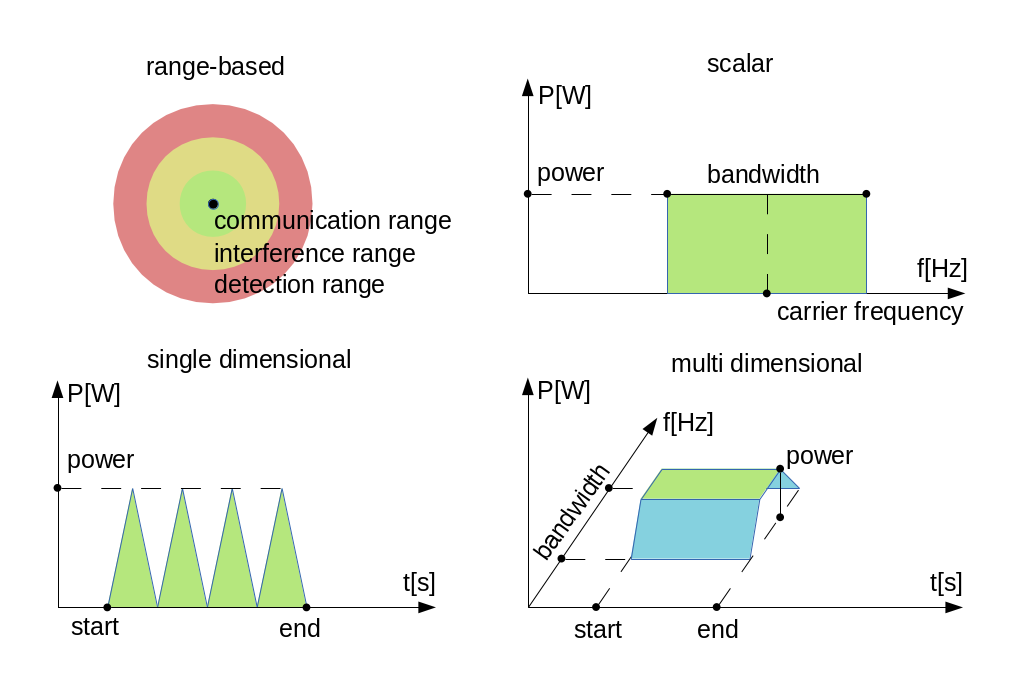
\includegraphics[width=\textwidth]{figures/phyanalog}
\caption{Various analog signal representations}
\end{figure}

The first representation is called range-based, and it's used by the unit disc
radio. The advantage of this data structure is that it's compact, predictable,
and provides high performance. The disadvantage is that it's very inaccurate in
terms of modeling reality. Nevertheless, this representation might be sufficient
for developing a new routing protocol if accurate simulation of packet loss is
not important.

The second data structure represents a narrowband signal with a scalar signal
power, a carrier frequency, and a bandwidth. The advantage of this
representation is that it allows to compute a real signal to noise ratio, which
in turn can be used by the error model to compute bit and packet error rates.
This representation is most of the time sufficient for the simulation of IEEE
802.11 networks.

The third data structure describes a signal power that changes over time. In
this case the signal power is represented with a one-dimensional time dependent
value that precisely follows the transmitted pulses. This representation is used
by the IEEE 802.15.4a UWB radio.

The last representation uses a multi-dimensional value to describe the signal
power that changes over both time and frequency. The IEEE 802.11b model might
use this representation to simulate crosstalk, where one channel interferes with
another. In order to make it work the frequency spectrum of the signal has to
follow the real spectrum more precisely at both ends of the band.

The flat signal representation uses a single object to simulatenously describe
all domains of the transmission or the reception. In contrast, the layered
signal representation uses one object to describe every domain seperately. The
advantage of the latter is that it's extensible with alternative implementations
for each domain. The disadvantage is that it needs more allocation and resource
management.

\section{Signal Processing}

The following figure shows the process of how a MAC packet gets from the
transmitter radio through the medium to the receiver radio. The figure focues on
how data flows between the processing components of the physical layer. The blue
boxes represent the data structures, and the red boxes represent the processing
components.

\begin{figure}[h!]
\centering
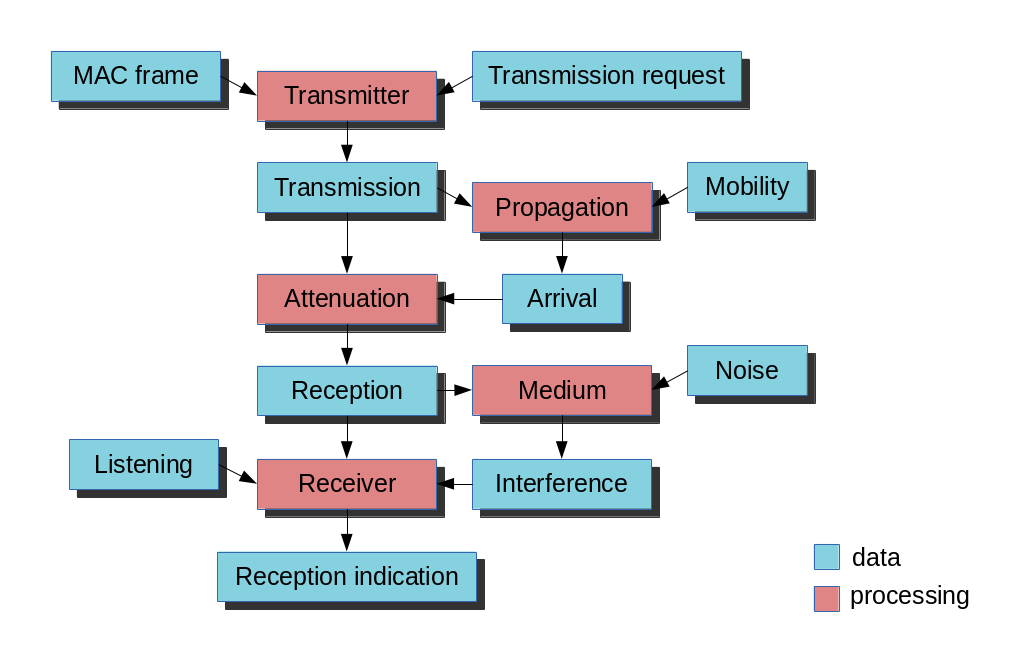
\includegraphics[width=\textwidth]{figures/phydataflow}
\caption{Signal processing data flow}
\end{figure}

The transmission process starts in the transmitter radio when it receives a MAC
packet from the higher layer. The radio must be in transmitter or transceiver
mode before receiving a MAC packet, otherwise it throws an exception. At first
the transmitter model creates a data structure that describes the transmitted
signal based on the received MAC packet and the attached transmission request.
The resulting data structure is immutable, it's not going to be changed in any
later processing step.

Thereafter the propagation model computes the arrival space-time coordinates for
all receivers. In the next step the medium model determines the set of affected
receivers. Which radio constitutes affected depends on a number of factors such
as the maximum communication range of the transmitter, the radio mode of the
receiver, the listening mode of the receiver, or potentially the MAC address of
the receiver. Using the result the medium model sends a separate message with
the shared transmission data structure to all affected receivers. There's no
need to send a message to all radios on the channel, because the computation
of interfering signals is independent of this step.

Thereafter the attenuation model computes the reception for the receiver using
the original transmission and the arrival data structure. It applies the path
loss model, the obstacle loss model and the multipath model to the transmission.
The resulting data structure is also immutable, it's not going to be changed in
any later processing step.

Thereafter the medium model computes the interference for the reception by
collecting all interfering receptions and noises. Another signal is considered
interfering if it owerlaps both in time and frequency domains with respect to 
the minimum interference parameters. The background noise model also computes a 
noise signal that is added to the interference.

The reception process starts in the receiver radio when it receives a message
from the transmitter radio. The radio must be in receiver or transceiver mode
before the message arrives, otherwise it ignores the message. At first the
receiver model determines is whether the reception is actually attempted or not.
This decision depends on the reception power, whether there's another ongoing
reception process, and capturing is enabled or not.

Thereafter the receiver model computes the signal to noise and interference
ratio from the reception and the interference. Using the result, the bitrate,
and the modulation scheme the error model computes the necessary error rates.
Alternatively the error model might compute the erroneous bits, or symbols by
altering the corresponding data of the original transmission. 

Thereafter the receiver determines the received MAC packet by either simply
reusing the original, or actually decoding from the lowest represented domain
in the reception. Finally, it attaches the physical layer indication to the MAC
packet, and sends it up to the higher layer.

The following sections describe the data structures that are created during
signal processing.

\subsubsection{Transmission Request}

This data structure contains parameters that control how the transmitter
produces the transmission. For example, it might override the default
transmission power, ot the default bitrate of the transmitter. It is attached as
a control info object to the MAC packet sent down from the MAC module to the
radio.

\subsubsection{Transmission}

This data structure describes the transmission of a signal. It specifies the
start/end time, start/end antenna position, start/end antenna orientation of the
transmitter. In other words, it describes when, where and how the signal
started/ended to interact with the medium. The transmitter model creates one
transmission instance per MAC packet.

\subsubsection{Arrival}

This data structure decscirbes the space and time coordinates of a transmission
arriving at a particular receiver. It specifies the start/end time, start/end
antenna position, start/end antenna orientation of the receiver. The propagation
model creates one arrival instance per transmission per receiver.

\subsubsection{Listening}

This data structure describes the way the receiver radio is listening on the
medium. The physical layer ignores certain transmissions either during computing
the interference or even the complete reception of such transmissions. For
example, a narrowband listening specifies a carrier frequency and a bandwidth. 

\subsubsection{Reception}

This data structure describes the reception of a signal by a particular receiver.
It specifies at least the start/end time, start/end antenna position, start/end
antenna orientation of the receiver. The attenuation model creates one reception
instance per transmission per receiver.

\subsubsection{Noise}

This data structure describes a meaningless signal or a meaningless composition
of multiple signals. All models contain at least the start/end time, and
start/end position.

\subsubsection{Interference}

This data structure describes the interfering signals and noises that affect a
particular reception. It also specifies the total noise that is the composition
of all interference.

\subsubsection{SNIR}

This data structure describes the signal to noise and interference ratio of a
particular reception. It also specifies the minimum signal to noise and
interference ratio.

\subsubsection{Reception Decision}

This data structure describes whether if the reception of a signal is possible
or not, is attempted or not, and is successful or not.

\subsubsection{Reception Indication}

This data structure describes the physical layer indications such as RSSI, SNIR,
PER, BER, SER. These physical properties are optional and may be omitted if the
receiver is configured to do so or if it doesn't support providing the data. The
reception indication is attached as a control info object to the MAC packet sent
up from the radio to the MAC module. 

\section{Visualization}

In order to help understanding the communication in the network the physical
layer supports visualizing its state. The following list shows what can be
displayed:

\begin{itemize}
  \item ongoing transmissions
  \item recent successful receptions
  \item recent obstacle intersections and surface normal vectors
\end{itemize}

The ongoing transmissions can be displayed with 3 dimensional spheres or with 2
dimensional rings laying in the XY plane. As the signal propagates through space
the figure grows with it to show where the beginning of the signal is. The inner
circle of the ring figure shows as the end of the signal propagates through
space. 

The recent successful receptions are displayed as straight lines between the
original positions of the transmission and the reception. The recent obstacle
intersections are also displayed as straight lines from the start of the
intersection to the end of it.

\section{TODO other stuff}

TODO: scalar vs dimensional

TODO: flat vs layered

TODO: Generic, IEEE 802.11, IEEE 802.15.4

TODO: acoustic underwater example

TODO: wireless vs. wired medium

\section{Use Cases}

\fi


\cleardoublepage

\chapter{The Transmission Medium}
\label{cha:transmission-medium}

\section{Overview}
\label{sec:medium:overview}

For wireless communication, an additional module is required to model the
shared physical medium where the communication takes place. This module
keeps track of transceivers, noise sources, ongoing transmissions,
background noise, and other ongoing noises.

It relies on several models:

\begin{enumerate}
  \item signal propagation model
  \item path loss model
  \item obstacle loss model
  \item background noise model
  \item signal analog model
\end{enumerate}

With the help of the above models, the medium module computes
when, where, and how signals arrive at receivers, including
the set of interfering signals and noises. In addition,
the medium module also contains various mechanisms and ways
to improve the scalability of wireless network simulations.

\section{RadioMedium}
\label{sec:medium:radiomedium}

The standard transmission medium model in INET is \nedtype{RadioMedium}.
\nedtype{RadioMedium} is as an OMNeT++ compound module with
several replaceable submodules. It contains submodules for
each of the above models (signal propagation, path loss, etc.),
and various caches for efficiency.

Note that \nedtype{RadioMedium} is an active compound module, that is,
it has an associated C++ class that encapsulates the computations.

\nedtype{RadioMedium} contains its components as submodules
with parametric types:

\begin{ned}
propagation: <propagationType> like IPropagation;
analogModel: <analogModelType> like IAnalogModel;
backgroundNoise: <backgroundNoiseType> like IRadioBackgroundNoise
    if backgroundNoiseType != "";
pathLoss: <pathLossType> like IPathLoss;
obstacleLoss: <obstacleLossType> like IObstacleLoss
    if obstacleLossType != "";
mediumLimitCache: <mediumLimitCacheType> like IMediumLimitCache;
communicationCache: <communicationCacheType> like ICommunicationCache;
neighborCache: <neighborCacheType> like INeighborCache
    if neighborCacheType != "";
\end{ned}

There are many preconfigured versions of \nedtype{RadioMedium}:

\begin{itemize}
  \item For use with \nedtype{UnitDiskRadio}: \nedtype{UnitDiskRadioMedium}
  \item For APSK radios: \nedtype{ApskScalarRadioMedium}, \nedtype{ApskDimensionalRadioMedium},
    \nedtype{ApskLayeredScalarRadioMedium}, \nedtype{ApskLayeredDimensionalRadioMedium},
  \item For IEEE 802.11: \nedtype{Ieee80211ScalarRadioMedium}, \nedtype{Ieee80211DimensionalRadioMedium},
    \nedtype{Ieee80211LayeredScalarRadioMedium}, \nedtype{Ieee80211LayeredDimensionalRadioMedium},
  \item For IEEE 802.15.4: \nedtype{Ieee802154UwbIrRadioMedium}, \nedtype{Ieee802154NarrowbandScalar\-RadioMedium}
\end{itemize}

The following sections describe the parts of the medium model.

\section{Propagation Models}
\label{sec:medium:propagation-models}

When a transmitter starts to transmit a signal, the beginning of the signal
propagates through the transmission medium. When the transmitter ends the
transmission, the signal's end propagates similarly. The propagation model
describes how a signal moves through space over time. Its main purpose is
to compute the arrival space-time coordinates at receivers. There are two
built-in models in INET, implemented as simple modules:

\begin{itemize}
        \item \nedtype{ConstantTimePropagation} is a simplistic model where the propagation time is independent of the traveled distance. The propagation time is simply determined by a module parameter.
        \item \nedtype{ConstantSpeedPropagation} is a more realistic model where the propagation time is proportional to the traveled distance. The propagation time is independent of the transmitter and receiver movement during both signal transmission and propagation. The propagation speed is determined by a module parameter.
\end{itemize}

The default propagation model is configured as follows:

\inisnippet{PropagationModelConfigurationExample}{Propagation model configuration example}

A more accurate model could take into consideration the transmitter and
receiver movement. This effect becomes especially important for acoustic
communication, because the propagation speed of the signal is much more
comparable to the speed of the transceivers.

\section{Path Loss Models}
\label{sec:medium:path-loss-models}

As a signal propagates through space its power density decreases. This is
called path loss and it is the combination of many effects such as
free-space loss, refraction, diffraction, reflection, and absorption. There
are several different path loss models in the literature, which differ in
their parameterization and application area.

In INET, a path loss model is an OMNeT++ simple module implementing a
specific path loss algorithm. Its main purpose is to compute the power loss
for a given signal, but it is also capable of estimating the range for a
given loss. The latter is useful, for example, to allow visualizing
communication range. INET contains a number of built-in path loss
algorithms, each comes with its own set of parameters:

\begin{itemize}
        \item \nedtype{FreeSpacePathLoss} models line of sight path loss for air or vacuum.
        \item \nedtype{BreakpointPathLoss} refines it using dual slope model with two separate path loss exponents.
        \item \nedtype{LogNormalShadowing} models path loss for a wide range of environments (e.g. urban areas, and buildings)
        \item \nedtype{TwoRayGroundReflection} models interference between line of sight and single ground reflection.
        \item \nedtype{TwoRayInterference} refines the above for inter-vechicle communication.
        \item \nedtype{RicianFading} is a stochastical model for the anomaly caused by partial cancellation of a signal by itself.
        \item \nedtype{RayleighFading} is a stochastical model for heavily built-up urban environments when there is no dominant propagation along the line of sight.
        \item \nedtype{NakagamiFading} further refines the above two models for cellular systems.
\end{itemize}

The following example replaces the default free-space path loss model with
log normal shadowing:

\inisnippet{PathLossConfigurationExample}{Path loss configuration example}

\section{Obstacle Loss Models}
\label{sec:medium:obstacle-loss-models}

When the signal propagates through space it also passes through physical
objects present in that space. As the signal penetrates physical objects,
its power decreases when it reflects from surfaces, and also when it is
absorbed by their material. There are various ways to model this effect,
which differ in the trade-off between accuracy and performance.

In INET, an obstacle loss model is an OMNeT++ simple module. Its main
purpose is to compute the power loss based on the traveled path and the
signal frequency. The obstacle loss models most often use the physical
environment model to determine the set of penetrated physical objects.
INET contains a few built-in obstacle loss models:

\begin{itemize}
        \item \nedtype{IdealObstacleLoss} model determines total or no power loss at all by checking if there is any obstructing physical object along the straight propagation path.
        \item \nedtype{DielectricObstacleLoss} computes the power loss based on the accurate dielectric and reflection loss along the straight path considering the shape, position, orientation, and material of obstructing physical objects.
\end{itemize}

By default, the medium module doesn't contain any obstacle loss model, but
configuring one is very simple:

\inisnippet{ObstacleLossModelConfigurationExample}{Obstacle loss model configuration example}

Statistical obstacle loss models are also possible but currently not provided.

\section{Background Noise Models}
\label{sec:medium:background-noise-models}

Thermal noise, cosmic background noise, and other random fluctuations of
the electromagnetic field affect the quality of the communication channel.
This kind of noise doesn't come from a particular source, so it doesn't
make sense to model its propagation through space. The background noise
model describes instead how it changes over space and time.

In INET, a background noise model is an OMNeT++ simple module. Its main
purpose is to compute the analog representation of the background noise for
a given space-time interval. For example,
\nedtype{IsotropicScalarBackgroundNoise} computes a background noise that is
independent of space-time coordinates, and its scalar power is determined
by a module parameter.

The simplest background noise model can be configured as follows:

\inisnippet{BackgroundNoiseModelConfigurationExample}{Background noise model configuration example}

\section{Analog Models}
\label{sec:medium:analog-models}

The analog signal is a complex physical phenomenon which can be modeled in
many different ways. Choosing the right analog domain signal representation
is the most important factor in the trade-off between accuracy and
performance. The analog model of the transmission medium determines how
signals are represented while being transmitted, propagated, and received.

In INET, an analog model is an OMNeT++ simple module. Its main purpose is
to compute the received signal from the transmitted signal. The analog
model combines the effect of the antenna, path loss, and obstacle loss
models. Transceivers must be configured transmit and receive signals
according to the representation used by the analog model.

The most commonly used analog model, which uses a scalar signal power
representation over a frequency and time interval, can be configured as
follows:

\inisnippet{AnalogModelConfigurationExample}{Analog model configuration example}

\section{Neighbor Cache}
\label{sec:medium:neighbor-cache}

Transceivers are considered neighbors if successful communication is
possible between them. For wired communication it is easy to determine
which transceivers are neighbors, because they are connected by wires. In
contrast, in wireless communication determining which transceivers are
neighbors isn't obvious at all.

In INET, a neighbor cache is an OMNeT++ simple module which provides
an efficient way of keeping track of the neighbor relationship between
transceivers. Its main purpose is to compute the set of affected receivers
for a given transmission. All built-in models in INET provide a
conservative approximation only, because they update their state
periodically:

\begin{itemize}
  \item \nedtype{NeighborListNeighborCache} takes a range as parameter,
    and for each transceiver it maintains the list of receivers within
    range (\textit{neighbor list}).
  \item \nedtype{GridNeighborCache} organizes transceivers in a 3D grid with
    constant cell size.
  \item \nedtype{QuadTreeNeighborCache} organizes transceivers in a 2D quad tree
    (ignoring the Z axis) with constant node size.
\end{itemize}

The following example sets \nedtype{QuadTreeNeighborCache} as neighbor cache:

\inisnippet{NeighborCacheModelConfigurationExample}{Neighbor cache model configuration example}

How should one decide which neighbor cache to choose for a given simulation?
As the sole purpose of the neighbor cache is to speed up the simulation,
one should choose the one that leads to the best performance for that particular
network. Which one performs best is best determined by experimentation, as it
depends on many factors: number of nodes, their spatial distribution, their
speed and movement pattern, their communication pattern, and so on.
Note that not only the choice of neighbor cache but also its parameterization
can affect performance.


\section{Medium Limit Cache}
\label{sec:medium:medium-limit-cache}

The medium limit cache (and its default implementation \nedtype{MediumLimitCache})
keeps track of certain thresholds and minimum/maximum values of quantities
related to layer 1 modeling. Some of these limits can be gathered from other
modules in the network, but still, all of them can be explicitly specified by the user.
The quantities include:

\begin{itemize}
    \item maximum speed (can be gathered from mobility models)
    \item maximum transmission power
    \item minimum interference power and reception power
    \item maximum antenna gain (can be computed from antenna models)
    \item minimum time interval to consider two overlapping signals interfering
    \item maximum duration of a transmission
    \item maximum communication range and interference range
      (can be computed from transmitter and receiver models)
\end{itemize}

These limits allow the transmission medium model to make assumptions about the
locations of nodes (i.e. the maximum distance they can move during some
interval), about the possibility of interference, and about the possibility
of a signal being receivable.


\section{Communication Cache}
\label{sec:medium:communication-cache}

The communication cache is used to cache various intermediate computation
results related to the communication on the medium. The main motivation to have
multiple implementations is that different implementations may be the most
efficient in different simulations. Also, a conservative (simple but robust)
implementation may be used for validating new (more efficient but also more
complex) implementations.

Implementations include:

\begin{itemize}
  \item \nedtype{ReferenceCommunicationCache}
  \item \nedtype{MapCommunicationCache}
  \item \nedtype{VectorCommunicationCache}
\end{itemize}


\section{Improving Scalability}
\label{sec:medium:improving-scalability}

The simulation of wireless networks is inherently less scalable than
that of wired networks. In wired networks, a transmission only affects
the host's neighbors on the link, which is usually 1 in modern networks
that are dominated by point-to-point links. The wireless medium, however,
is a broadcast medium. Any transmission is ``heard'' by all nodes
within interference range, not only the intended recipients.
The signal may be receivable by them (and must be indeeded received
before the destination address field in it can be examined),
or may interfere with the reception of other transmissions.
Whichever the case, the transmission must be evaluated or processed
by a much larger number of nodes than in the wired case.
This makes the computational complexity at least $O(n^2)$ ($n$ being
the number of nodes.) Other effects may further increase the exponent.

The medium module provides a set of parameters that can be used
to alleviate the scalability issue. These \textit{filter} parameters
that can be used to reduce the amount of processing at nodes that are
not the indended recipients of the frame, increasing simulation performance.

There are several filters that can be enabled/disabled individually:

\begin{itemize}
  \item \textit{Range filter}. When this filter is active, the medium module
    does not send signals to a radio if it is outside interference range
    (or communication range, this option can also be selected.)
  \item \textit{Radio mode filter}. When this filter is active,
    the medium module does not send signals to a radio if it is neither
    in \textit{receiver} nor in \textit{transceiver} mode.
  \item \textit{Listening filter}. When this filter is active, the medium module
    does not send signals to a radio if it listens on the channel in
    incompatible mode (e.g. different carrier frequency and bandwidth,
    or different modulation)
  \item \textit{MAC address filter}. When this filter is active, the radio medium
    does not send signals to a radio if it the destination MAC address
    does not match
\end{itemize}

The corresponding module parameters are called \ttt{rangeFilter},
\ttt{radioModeFilter}, \ttt{listeningFilter} and \ttt{macAddressFilter}.
By default, all filters are turned off.

%%% Local Variables:
%%% mode: latex
%%% TeX-master: "usman"
%%% End:

\cleardoublepage

\ifdraft TODO

\chapter{The Physical Environment}
\label{cha:environment}

TODO C++ interface

\fi



\cleardoublepage

\chapter{Node Mobility}
\label{cha:mobility}

\section{Overview}
\label{sec:mobility:overview}

In order to simulate ad-hoc wireless networks, it is important to model the
motion of mobile network nodes. Received signal strength, signal
interference, and channel occupancy depend on the distances between nodes.
The selected mobility models can significantly influence the results of the
simulation (e.g. via packet loss rates).

A mobility model describes position and orientation over time in a 3D
Euclidean coordinate system. Its main purpose is to provide position,
velocity and acceleration, and also angular position, angular velocity,
and angular acceleration data as three-dimensional quantities at the
current simulation time.

In INET, a mobility model is most often an OMNeT++ simple module
implementing the motion as a C++ algorithm. Although most models have a few
common parameters (e.g. for initial positioning), they always come with
their own set of parameters. Some models support geographic positioning to
ease the configuration of map based scenarios.

Mobility models be \textit{single} or \textit{group} mobility models.
Single mobility models describe the motion of entities independent of each other.
Group mobility models provide such a motion where group members are dependent
on each other.

Mobility models can also be categorized as \textit{trace-based},
\textit{deterministic}, \textit{stochastic}, and \textit{combining} models.

\subsection*{Using Mobility Models}

In order for a mobility model to actually have an effect on the motion of a network node,
the mobility model needs to be included as a submodule in the compound module of the
network node. By default, a transceiver antenna within a network node uses
the same mobility model as the node itself, but that is completely optional.
For example, it is possible to model a vehicle facing forward while moving
on a road that contains multiple transceiver antennas at different relative
locations with different orientations.

\subsection*{The Playground}

Many mobility models allow the user to define a cubic volume that the node
can not leave. The volume is configured by setting the \fpar{constraintAreaX},
\fpar{constraintAreaY}, \fpar{constraintAreaZ},
\fpar{constraintAreaWidth}, \fpar{constraintAreaHeight} and
\fpar{constraintAreaDepth} parameters.

If the \fpar{initFromDisplayString} parameter, the initial position is taken from
the display string. Otherwise, the position can be given in the \fpar{initialX},
\fpar{initialY} and \fpar{initialZ} parameters. If neither of these parameters
are given, a random initial position is choosen within the contraint area.

When the node reaches the boundary of the constraint area, the mobility
component has to prevent the node to exit. Many mobility models offer the
following policies:

\begin{itemize}
  \item reflect of the wall
  \item reappear at the opposite edge (torus area)
  \item placed at a randomly chosen position of the area
  \item stop the simulation with an error
\end{itemize}


\section{Built-In Mobility Models}
\label{sec:mobility:built-in-mobility-models}

\subsection{List of Mobility Models}
\label{sec:mobility:list-of-mobility-models}

The following, potentially list contains the mobility models available in INET.
Nearly all of these models als single mobility models; group mobility can be
implemented e.g. with combining other mobility models.

\subsubsection*{Stationary}

Stationary models only define position (and orientation), but no motion.

\begin{itemize}
    \item \nedtype{StationaryMobility} provides deterministic and random positioning.
    \item \nedtype{StaticGridMobility} places several mobility models in a rectangular grid.
    \item \nedtype{StaticConcentricMobility} places several models in a set of concentric circles.
\end{itemize}

\subsubsection*{Deterministic}

Deterministic mobility models use non-random mathematical models for describing motion.

\begin{itemize}
    \item \nedtype{LinearMobility} moves linearly with a constant speed or constant acceleration.
    \item \nedtype{CircleMobility} moves around a circle parallel to the XY plane with constant speed.
    \item \nedtype{RectangleMobility} moves around a rectangular area parallel to the XY plane with constant speed.
    \item \nedtype{TractorMobility} moves similarly to a tractor on a field with a number of rows.
    \item \nedtype{VehicleMobility} moves similarly to a vehicle along a path especially turning around corners.
    \item \nedtype{TurtleMobility} moves according to an XML script written in a simple yet expressive LOGO-like programming language.
    \item \nedtype{FacingMobility} orients towards the position of another mobility model.
    \item \nedtype{RotatingMobility} rotates with a constant speed.
\end{itemize}

\subsubsection*{Trace-Based}

Trace-based mobility models replay recorded motion as observed in real life.

\begin{itemize}
    \item \nedtype{BonnMotionMobility} replays trace files of the BonnMotion scenario generator.
    \item \nedtype{Ns2MotionMobility} replays files of the CMU's scenario generator used in ns2.
    \item \nedtype{AnsimMobility} replays XML trace files of the ANSim (Ad-Hoc Network Simulation) tool.
\end{itemize}

\subsubsection*{Stochastic}

Stochastic or random mobility models use mathematical models involving random numbers.

\begin{itemize}
    \item \nedtype{RandomWaypointMobility} moves to random destination with random speed.
    \item \nedtype{GaussMarkovMobility} uses one parameter to vary the degree of randomness from linear to Brown motion.
    \item \nedtype{MassMobility} moves similarly to a mass with inertia and momentum.
    \item \nedtype{ChiangMobility} uses a probabilistic transition matrix to change the motion state.
\end{itemize}

\subsubsection*{Combining}

Combining mobility models are not mobility models per se, but instead, they
allow more complex motions to be formed from simpler ones via superposition
and other ways.

\begin{itemize}
        \item \nedtype{SuperpositioningMobility} model combines several other mobility models by summing them up. It allows creating group mobility by sharing a mobility model in each group member, separating initial positioning from positioning during the simulation, and separating positioning from orientation.
        \item \nedtype{AttachedMobility} models a mobility that is attached to another one at a given offset. Position, velocity and acceleration are all affected by the respective quantites and also the orientation of the referenced mobility.
\end{itemize}

\subsection{More Information on Some Mobility Models}
\label{sec:mobility:more-information-on-some-mobility-models}

\subsubsection*{TractorMobility}

Moves a tractor through a field with a certain
amount of rows. The following figure illustrates the movement of the
tractor when the \fpar{rowCount} parameter is 2. The trajectory follows
the segments in $1,2,3,4,5,6,7,8,1,2,3\ldots$ order. The area is configured
by the \fpar{x1}, \fpar{y1}, \fpar{x2}, \fpar{y2} parameters.

% TODO use constraint area instead of new x1,y1,x2,y2 parameters as in RectangleMobility

\begin{pdfonly}
\begin{center}
\setlength{\unitlength}{0.5mm}
\begin{picture}(80,80)
\put(40,72){$1$} \put(10,70){\vector(1,0){30}} \put(10,70){\line(1,0){60}}
\put(72,55){$2$} \put(70,70){\vector(0,-1){15}} \put(70,70){\line(0,-1){30}}
\put(40,42){$3$} \put(70,40){\vector(-1,0){30}} \put(70,40){\line(-1,0){60}}
\put(5,25){$4$} \put(10,40){\vector(0,-1){15}} \put(10,40){\line(0,-1){30}}
\put(40,12){$5$} \put(10,10){\vector(1,0){30}} \put(10,10){\line(1,0){60}}
\put(72,25){$6$} \put(70,10){\vector(0,1){15}} \put(70,10){\line(0,1){30}}
\put(40, 33){$7$}
\put(5,55){$8$} \put(10,40){\vector(0,1){15}} \put(10,40){\line(0,1){30}}
\put(0,72){$(x_1,y_1)$} \put(65,2){$(x_2,y_2)$}
\end{picture}
\end{center}
\end{pdfonly}

\begin{htmlonly}
<center><img src="tractormobility.png" border="0" width="240"></center> <!-- screenshot from the PDF version -->
\end{htmlonly}

\subsubsection*{RandomWaypointMobility}

In the Random Waypoint mobility model the nodes move in line segments. For each
line segment, a random destination position (distributed uniformly over the
playground) and a random speed is chosen. You can define a speed as a variate
from which a new value will be drawn for each line segment; it is customary to
specify it as \ttt{uniform(minSpeed, maxSpeed)}. When the node reaches the
target position, it waits for the time \fpar{waitTime} which can also be defined as a
variate. After this time the the algorithm calculates a new random position, etc.

\subsubsection*{GaussMarkovMobility}

The Gauss-Markov model contains a tuning parameter that control the randomness
in the movement of the node. Let the magnitude and direction of speed of the
node at the $n$th time step be $s_n$ and $d_n$. The next speed and direction are
computed as

$$ s_{n+1} = \alpha s_n + (1 - \alpha) \bar{s} + \sqrt{(1-\alpha^2)} s_{x_n} $$

$$ d_{n+1} = \alpha s_n + (1 - \alpha) \bar{d} + \sqrt{(1-\alpha^2)} d_{x_n} $$

where $\bar{s}$ and $\bar{d}$ are constants representing the mean value
of speed and direction as $n \to \infty$; and $s_{x_n}$ and $d_{x_n}$
are random variables with Gaussian distribution.

Totally random walk (Brownian motion) is obtained by setting $\alpha=0$,
while $\alpha=1$ results a linear motion.

To ensure that the node does not remain at the boundary of the constraint
area for a long time, the mean value of the direction ($\bar{d}$) modified
as the node enters the margin area. For example at the right edge of the
area it is set to 180 degrees, so the new direction is away from the edge.

\subsubsection*{MassMobility}

This is a random mobility model for a mobile host with
a mass. It is the one used in \cite{Perkins99optimizedsmooth}.

\begin{quote}
"An MH moves within the room according to the following pattern. It moves
along a straight line for a certain period of time before it makes a turn.
This moving period is a random number, normally distributed with average of
5 seconds and standard deviation of 0.1 second. When it makes a turn, the
new direction (angle) in which it will move is a normally distributed
random number with average equal to the previous direction and standard
deviation of 30 degrees. Its speed is also a normally distributed random
number, with a controlled average, ranging from 0.1 to 0.45 (unit/sec), and
standard deviation of 0.01 (unit/sec). A new such random number is picked
as its speed when it makes a turn. This pattern of mobility is intended to
model node movement during which the nodes have momentum, and thus do not
start, stop, or turn abruptly. When it hits a wall, it reflects off the
wall at the same angle; in our simulated world, there is little other
choice."
\end{quote}

This implementation can be parameterized a bit more, via the
\fpar{changeInterval}, \fpar{changeAngleBy} and \fpar{changeSpeedBy} parameters.
The parameters described above correspond to the following settings:

\begin{itemize}
\item changeInterval = normal(5, 0.1)
\item changeAngleBy = normal(0, 30)
\item speed = normal(avgSpeed, 0.01)
\end{itemize}

\subsubsection*{ChiangMobility}

Implements Chiang's random walk movement model (\cite{Chiang98wirelessnetwork}).
In this model, the state of the mobile node in each direction (x and y) can be:

\begin{itemize}
  \item 0: the node stays in its current position
  \item 1: the node moves forward
  \item 2: the node moves backward
\end{itemize}

The $(i,j)$ element of the state transition matrix determines the
probability that the state changes from $i$ to $j$:

\begin{pdfonly}
$$ \left(
\begin{array}{ccc}
  0 & 0.5 & 0.5 \\
  0.3 & 0.7 & 0 \\
  0.3 & 0 & 0.7
\end{array}
\right) $$
\end{pdfonly}

\begin{htmlonly}
<center>
<div>
<table class="matrix">
  <tr> <td>0</td>   <td>0.5</td> <td>0.5</td> </tr>
  <tr> <td>0.3</td> <td>0.7</td> <td>0</td>   </tr>
  <tr> <td>0.3</td> <td>0</td>   <td>0.7</td> </tr>
</table>
</div>
</center>
\end{htmlonly}

\subsection{Replaying trace files}
\label{sec:mobility:replaying-trace-files}

\subsubsection*{BonnMotionMobility}

Uses the native file format of \href{http://bonnmotion.net}{BonnMotion}.

The file is a plain text file, where every line describes the motion
of one host. A line consists of one or more (t, x, y) triplets of real
numbers, like:

\begin{verbatim}
t1 x1 y1 t2 x2 y2 t3 x3 y3 t4 x4 y4 ...
\end{verbatim}

The meaning is that the given node gets to $(xk,yk)$ at $tk$. There's no
separate notation for wait, so x and y coordinates will be repeated there.

\subsubsection*{Ns2MotionMobility}

Nodes are moving according to the trace files used in NS2.
The trace file has this format:

\begin{verbatim}
# '#' starts a comment, ends at the end of line
$node_(<id>) set X_ <x> # sets x coordinate of the node identified by <id>
$node_(<id>) set Y_ <y> # sets y coordinate of the node identified by <id>
$node_(<id>) set Z_ <z> # sets z coordinate (ignored)
$ns at $time "$node_(<id>) setdest <x> <y> <speed>" # at $time start moving
towards <x>,<y> with <speed>
\end{verbatim}

The \nedtype{Ns2MotionMobility} module has the following parameters:

\begin{itemize}
  \item \fpar{traceFile} the Ns2 trace file
  \item \fpar{nodeId} node identifier in the trace file; -1 gets substituted by
  parent module's index
  \item \fpar{scrollX},\fpar{scrollY} user specified translation of the
  coordinates
\end{itemize}

% TODO cleaning the code (e.g. duplicated bounds check in setTargetPosition())
% TODO implement cached file access as in BonnMotionMobility

\subsubsection*{ANSimMobility}

It reads trace files of the \href{http://www.ansim.info}{ANSim} Tool.
The nodes are moving along linear segments described by an XML trace file
conforming to this DTD:

\begin{XML}
<!ELEMENT mobility (position_change*)>
<!ELEMENT position_change (node_id, start_time, end_time, destination)>
<!ELEMENT node_id (#PCDATA)>
<!ELEMENT start_time (#PCDATA)>
<!ELEMENT end_time (#PCDATA)>
<!ELEMENT destination (xpos, ypos)>
<!ELEMENT xpos (#PCDATA)>
<!ELEMENT ypos (#PCDATA)>
\end{XML}

Parameters of the module:

\begin{itemize}
  \item \fpar{ansimTrace} the trace file
  \item \fpar{nodeId} the \verb!node_id! of this node, -1 gets substituted to
  parent module's index
\end{itemize}

\begin{note}
The \nedtype{AnsimMobility} module processes only the \ttt{position\_change}
elements and it ignores the \ttt{start\_time} attribute. It starts the move
on the next segment immediately.
\end{note}

\subsection{TurtleMobility}
\label{sec:mobility:turtlemobility}

The \nedtype{TurtleMobility} module can be parametrized by a script file
containing LOGO-style movement commands in XML format. The content of
the XML file should conform to the DTD in the \ffilename{TurtleMobility.dtd}
file in the source tree.

The file contains \ttt{movement} elements, each describing a trajectory.
The \ttt{id} attribute of the \ttt{movement} element can be used to
refer the movement from the ini file using the syntax:

\begin{inifile}
**.mobility.turtleScript = xmldoc("turtle.xml", "movements//movement[@id='1']")
\end{inifile}

The motion of the node is composed of uniform linear segments.
The \ttt{movement} elements may contain the the following commands as
elements (names in parens are recognized attribute names):

\begin{itemize}
\item \ttt{repeat(n)} repeats its content n times, or indefinitely if
       the \ttt{n} attribute is omitted.
\item \ttt{set(x,y,speed,angle,borderPolicy)} modifies the state of the node.
      \ttt{borderPolicy} can be \ttt{reflect}, \ttt{wrap}, \ttt{placerandomly}
      or \ttt{error}.
\item \ttt{forward(d,t)} moves the node for $t$ time or to the $d$ distance
      with the current speed. If both $d$ and $t$ is given, then the current
      speed is ignored.
\item \ttt{turn(angle)} increase the angle of the node by $angle$ degrees.
\item \ttt{moveto(x,y,t)} moves to point $(x,y)$ in the given time. If
      $t$ is not specified, it is computed from the current speed.
\item \ttt{moveby(x,y,t)} moves by offset $(x,y)$ in the given time. If
      $t$ is not specified, it is computed from the current speed.
\item \ttt{wait(t)} waits for the specified amount of time.
\end{itemize}

Attribute values must be given without physical units, distances are assumed
to be given as meters, time intervals in seconds and speeds in meter per seconds.
Attibutes can contain expressions that are evaluated each time the
command is executed. The limits of the constraint area can be
referenced as \verb!$MINX!, \verb!$MAXX!, \verb!$MINY!, and \verb!$MAXY!.
Random number distibutions generate a new random number when evaluated,
so the script can describe random as well as deterministic scenarios.

To illustrate the usage of the module, we show how some mobility
models can be implemented as scripts.

RectangleMobility:

\begin{XML}
<movement>
    <set x="$MINX" y="$MINY" angle="0" speed="10"/>
    <repeat>
        <repeat n="2">
            <forward d="$MAXX-$MINX"/>
            <turn angle="90"/>
            <forward d="$MAXY-$MINY"/>
            <turn angle="90"/>
        </repeat>
    </repeat>
</movement>
\end{XML}

Random Waypoint:

\begin{XML}
<movement>
    <repeat>
        <set speed="uniform(20,60)"/>
        <moveto x="uniform($MINX,$MAXX)" y="uniform($MINY,$MAXY)"/>
        <wait t="uniform(5,10)">
    </repeat>
</movement>
\end{XML}

MassMobility:

\begin{XML}
<movement>
    <repeat>
        <set speed="uniform(10,20)"/>
        <turn angle="uniform(-30,30)"/>
        <forward t="uniform(0.1,1)"/>
    </repeat>
</movement>
\end{XML}


%%% Local Variables:
%%% mode: latex
%%% TeX-master: "usman"
%%% End:



\cleardoublepage

\chapter{Modeling Power Consumption}
\label{cha:power}

\section{Overview}
\label{sec:power:overview}

Modeling power consumption becomes more and more important with the increasing
number of embedded devices and the upcoming Internet of Things. Mobile personal
medical devices, large scale wireless environment monitoring devices, electric
vehicles, solar panels, low-power wireless sensors, etc. require paying special
attention to power consumption. The high fidelity simulation of power
consumption allows designing power sensitive routing protocols, MAC protocols,
physical layers, etc. which in turn results in more energy efficient devices.

In order to help the modeling process the power model is separated from other
simulation models. This separation makes the model extensible and it also allows
easy experimentation with alternative implementations. In a nutshell the power
model consists of the following components:

\begin{itemize}
  \item energy consumption models
  \item energy generation models
  \item temporary energy storage models
\end{itemize}

The power model elements fall into two categories, abbreviated with \ttt{Ep}
and \ttt{Cc} as part of their names:

\begin{itemize}
  \item \ttt{Ep} models are simpler, and deal with energy and power quantities.
  \item \ttt{Cc} models are more realistic, and deal with charge, current, and voltage quantities.
\end{itemize}

The following sections provide a brief overview of the power model.

\section{Energy Consumer Models}
\label{sec:power:energy-consumer-models}

Energy consumer models describe the energy consumption of devices over time.
For example, a transceiver consumes energy when it transmits or
receives signals, a CPU consumes energy when the network protocol routes
packets, and a display consumes energy when it's turned on.

In INET, an energy consumer model is an OMNeT++ simple module that implements
the energy consumption of software processes or hardware devices over time.
Its main purpose is to provide the power or current consumption for the
current simulation time. Most often energy consumers are included as
submodules in the compound module of the hardware devices or software
components.

INET provides only a few built-in energy consumer models:

\begin{itemize}
        \item \nedtype{AlternatingEpEnergyGenerator} is a trivial energy/power based statistical energy consumer model example.
        \item \nedtype{StateBasedEpEnergyConsumer} is a transceiver energy consumer model based on the radio mode and transmission/reception states.
\end{itemize}

In order to simulate power consumption in a wireless network, the energy
consumer model type must be configured for the transceivers. The following
example demonstrates how to configure the power consumption parameters for
a transceiver energy consumer model:

\inisnippet{EnergyConsumerConfigurationExample}{Energy consumer configuration example}


\section{Energy Generator Models}
\label{sec:power:energy-generator-models}

Energy generator models describe the energy generation of devices over time.
A solar panel, for example, produces energy based on time, the panel's
position on the globe, its orientation towards the sun and the actual weather
conditions. Energy generators connect to an energy storage that absorbs the
generated energy.

In INET, an energy generator model is an OMNeT++ simple module implementing
the energy generation of a hardware device using a physical phenomena over
time. Its main purpose is to provide the power or current generation for
the current simulation time. Most often energy generation models are
included as submodules in network nodes.

INET provides only one trivial energy/power based statistical energy
generator model called \nedtype{AlternatingEpEnergyGenerator}. The following
example shows how to configure its power generation parameters:

\inisnippet{EnergyGeneratorConfigurationExample}{Energy generator configuration example}

\section{Energy Storage Models}
\label{sec:power:energy-storage-models}

Electronic devices which are not connected to external power source must contain
some component to store energy. For example, an electrochemical battery in a
mobile phone provides energy for its display, its CPU, and its communication
devices. It might also absorb energy produced by a solar installed on its
display, or by a portable charger plugged into the wall socket.

In INET, an energy storage model is an OMNeT++ simple module which models
the physical phenomena that is used to store energy produced by generators
and provide energy for consumers. Its main purpose is to compute the amount
of available energy or charge at the current simulation time. It maintains
a set of connected energy consumers and energy generators, their respective
total power consumption and total power generation.

INET contains a few built-in energy storage models:

\begin{itemize}
        \item \nedtype{IdealEpEnergyStorage} is an idealistic model with infinite energy capacity and infinite power flow.
        \item \nedtype{SimpleEpEnergyStorage} is a non-trivial model integrating the difference between the total consumed power and the total generated power over time.
        \item \nedtype{SimpleCcBattery} is a more realistic charge/current based battery model using a charge independent ideal voltage source and internal resistance.
\end{itemize}

The following example shows how to configure a simple energy storage model:

\inisnippet{EnergyStorageConfigurationExample}{Energy storage configuration example}

\section{Energy Management Models}
\label{sec:power:energy-management-models}

% Why energy management models are needed?
% The energy management models monitors an energy storage, estimates its state, and controls the consumers and generators to protect the energy storage from operating outside its safe operating area.

\nedtype{SimpleEpEnergyManagement}

\inisnippet{EnergyManagementConfigurationExample}{Energy management configuration example}



%%% Local Variables:
%%% mode: latex
%%% TeX-master: "usman"
%%% End:


\cleardoublepage

\chapter{Network Emulation}
\label{cha:emulation}

\section{Motivation}
\label{sec:emulation:motivation}

There are several projects that may benefit from the network emulation
capabilities of INET, that is, from the ability to mix simulated components
with real networks.

Some example scenarios:

\begin{itemize}
  \item Run a simulated component, such as an app or a routing protocol,
    on nodes of an actual ad-hoc network. This setup would allow testing
    the component's behavior under real-life conditions.
  \item Test the interoperability of a simulated protocol with its real-world
    counterparts. Several setups are possible: simulated node in a real network;
    a simulated subnet in real network; real-world node in simulated network; etc.
  \item As a means of implementing hybrid simulation. The real network
    (or a single host OS) may contain several network emulator devices
    or simulations running in emulation mode. Such a setup provides a relatively
    easy way for connecting heterogenous simulators/emulators with each
    other, sparing the need for HLA or a custom interoperability solution.
\end{itemize}


\section{Overview}
\label{sec:emulation:overview}

To act as a network emulator, the simulation must run in real time,
and must be able to communicate with the real world.

% [Background] To understand how it works, first look at how
% a normal simulation is run. There is a scheduler which always
% returns the earliest event from the FES, and the simulation processes
% these events in as fast succession as possible.
%
% For real-time simulation, this scheduler is replaced with one
% augmented with wait calls (e.g. usleep()) that synchronize the
% simulation time to the system clock.
%
% For emulation, the real-time scheduler is augmented with code
% that captures packets from real network devices, and inserts
% them into the simulation.
%
% INET contains an emulation scheduler, which uses the pcap library
% to capture packets, and raw sockets to send packets to a real network device.
%

This is achieved with two components in INET:

\begin{itemize}
  \item \nedtype{ExtInterface} is an INET network interface that represents
    a real interface (an interface of the host OS) in the simulation.
    Packets sent to an \nedtype{ExtInterface} will be sent out on the
    host OS interface, and packets received by the host OS interface
    (or rather, the appropriate subset of them) will appear in the
    simulation as if received on an \nedtype{ExtInterface}. The code
    uses the pcap library for capturing packets, and raw sockets for sending.
 \item \cppclass{RealTimeScheduler}, a socket-aware real-time scheduler class.
\end{itemize}

\begin{note}
It is probably needless to say, but the simulation must be fast enough
to be able to keep up with real time. That is, its relative speed compared
to real time (the simsec/sec value) must be $>>1$.  (Under Qtenv, this
can usually only be achieved in Express mode.)
\end{note}

The simulation is run under Qtenv,

\section{Preparation}
\label{sec:emulation:preparation}

There are a few things that need to be arranged before you can successfully
run simulations in network emulation mode.

First, network emulation is a separate \textit{project feature} that needs to
be enabled before it can be used. (Project features can be reviewed and changed
in the \emph{Project | Project Features...} dialog in the IDE.)

The network emulation code makes use of the pcap library, and therefore
it must be available on your system. On Ubuntu, for example, pcap can be
installed with the following command:

\begin{verbatim}
$ sudo apt install libpcap-dev
\end{verbatim}

Also, when running a simulation, make sure you have the necessary permissions.
Sending uses raw sockets (type \ttt{SOCK\_RAW}), which, on many systems,
is only allowed for processes that have root (administrator) privileges.


\section{Configuring}
\label{sec:emulation:configuring}

INET nodes such as \nedtype{StandardHost} and \nedtype{Router}
can be configured to have \nedtype{ExtInterface}s.
The simulation may contain several nodes with external interfaces,
and one node may also have several external interfaces.

A network node can be configured to have an external interface
in the following way:

\begin{inifile}
**.host1.numExtInterfaces = 1
\end{inifile}

Also, the simulation must be configured to run under control the of the
appropriate real-time scheduler class:

\begin{inifile}
scheduler-class = "inet::RealTimeScheduler"
\end{inifile}

\nedtype{ExtInterface} has two important parameters which need to be
configured. The \fpar{device} parameter should be set to the name of the real
interface on the host OS, and \fpar{filterString} should contain a packet
filter expression that selects which packets captured on the real interface
should  be relayed into the simulation via this \nedtype{ExtInterface}.
(\fpar{filterString} is simply passed to the pcap library, so it should
follow the \textit{tcpdump} filter expressions syntax that pcap understands.)

An example configuration:

\begin{inifile}
**.numExtInterfaces = 1
**.ext[0].ext.filterString = "(sctp or icmp) and ip dst host 10.1.1.1"
**.ext[0].ext.device = "eth0" # or "en0" on macOS, or something
**.ext[0].ext.mtu = 1500B
\end{inifile}

The filter string \ttt{"(sctp or icmp) and ip dst host 10.1.1.1"} means
that the protocol must be SCTP or ICMP, and the destination host must be
10.1.1.1.

\begin{note}
Why is filtering of incoming packets done at packet capture (in pcap),
and not in \nedtype{ExtInterface}? The reason is performance: it costs
much fewer CPU cycles to discard unnecessary packets right where
they come in, and not send them up into the simulation for the
same decision. And, given that the simulation needs to keep up with
real time, saving CPU cycles is important.
\end{note}

Let us examine the paths outgoing and incoming packets take, and the
necessary configuration requirements to make them work. We assume IPv4
as network layer protocol, but the picture does not change much with
other protocols. We assume the external interface is named \ttt{ext[0]}.

\subsection*{Outgoing path}

The network layer of the simulated node routes datagrams to its
\ttt{ext[0]} external interface.

For that to happen, the routing table needs to contain an entry
where the interface is set to \ttt{ext[0]}. Such entries are
not created automatically, one needs to add them to the routing
table explicitly, e.g. by using an \nedtype{Ipv4NetworkConfigurator}
and an appropriate XML file.

Another point is that if the packet comes from a local app (and from
another simulated node), it needs to have a source IP address assigned.
There are two ways for that to happen. If the sending app specified
a source IP address, that will be used. Otherwise, the IP address
of the \ttt{ext[0]} interface will be used, but for that, the interface
needs to have an IP address at all.

Once in \ttt{ext[0]}, the datagram is serialized.
Serialization is a built-in feature of INET packets. (Packets, or rather,
packet chunks have multiple alternative representations, i.e. C++ object
and serialized form, and conversion between them is transparent.)

The result of serialization is a byte string, which is written into
a raw socket with a \ttt{sendto} system call.

% TODO this was true in 4.0 prereleases, hopefully fixed in final 4.0:
% The host OS will again route the packet, and send it out on the
% output interface determined by the packet's destination IP address.
% (Note that this may not be the same as the interface specified
% in \ttt{ext[0]}'s \fpar{device} parameter. Unfortunately,
% in the current implementation one raw socket is shared by
% all \nedtype{ExtInterface} instances which may have different
% \fpar{device} settings, so the socket cannot be bound to the
% real interface associated with originator \nedtype{ExtInterface}.)

The packet will then travel normally in the real network to the
destination address.

\subsection*{Incoming path}

First of all, packets intended to be received by the simulation
need to find their way to the correct  interface of the host that
runs the simulation. For that, IP addresses of simulated hosts
must be routable in the real network, and routed to the captured
interface of the host OS. (On Linux, for example, this can be achieved
by adding static routes with the \ttt{ip route add <prefix> via
<host>} command.)

As packets are received by the interface of the host OS, they
are examined by the pcap library to find out whether they match
the filter expression. If the filter matches, pcap hands the
packet over to the simulation, and after deserialization
it pops out of \ttt{ext[0]} and sent up to the network
layer. After that, it is routed to the simulated destination host
in the normal way.

The pcap filter expression must be crafted so that it matches
the packets destined to simulated hosts, and does not match
any other packet.

Moreover, if the simulation contains several external interfaces
that map to the same real interface, care must be taken so that
filter expressions are disjunct. Otherwise, a packet may be
matched by more than one filter, and then it will be inserted
into the simulation in multiple copies (once for each matching
\nedtype{ExtInterface}.) This is usually not what is wanted.

%%% Local Variables:
%%% mode: latex
%%% TeX-master: "usman"
%%% End:


\cleardoublepage

\chapter{Network Autoconfiguration}
\label{cha:network-autoconfiguration}

\section{Overview}
\label{sec:autoconfig:overview}

This chapter describes static autoconfiguration of networks.

\section{Configuring IPv4 Networks}
\label{sec:autoconfig:configuring-ipv4-networks}

An IPv4 network is composed of several nodes like hosts, routers,
switches, hubs, Ethernet buses, or wireless access points.
The nodes having a IPv4 network layer (hosts and routers) should be
configured at the beginning of the simulation. The configuration
assigns IP addresses to the nodes, and fills their routing tables.
If multicast forwarding is simulated, then the multicast routing
tables also must be filled in.

% TODO define nodes, IP nodes, routers, multicast routers

The configuration can be manual (each address and route is fully specified
by the user), or automatic (addresses and routes are generated by
a configurator module at startup).

Before version 1.99.4 INET offered \nedtype{Ipv4FlatNetworkConfigurator}
for automatic and routing files for manual configuration.
Both had serious limitations, so a new configurator has been added
in version 1.99.4: \nedtype{Ipv4NetworkConfigurator}. This configurator
supports both fully manual and fully automatic configuration. It
can also be used with partially specified manual configurations,
the configurator fills in the gaps automatically.

The next section describes the usage of \nedtype{Ipv4NetworkConfigurator}.
The legacy solutions \nedtype{Ipv4FlatNetworkConfigurator} and
routing files are described in subsequent sections.

\subsection{Ipv4NetworkConfigurator}
\label{sec:autoconfig:ipv4networkconfigurator}

The \nedtype{Ipv4NetworkConfigurator} assigns IP addresses and sets up
static routing for an IPv4 network.

It assigns per-interface IP addresses, strives to take subnets into account,
and can also optimize the generated routing tables by merging routing entries.

Hierarchical routing can be set up by using only a fraction of configuration
entries compared to the number of nodes. The configurator also does
routing table optimization that significantly decreases the size of routing
tables in large networks.

The configuration is performed in stage 2 of the initialization. At this
point interface modules (e.g. PPP) has already registered their interface
in the interface table. If an interface is named \ttt{ppp[0]}, then the
corresponding interface entry is named \ttt{ppp0}. This name can be used
in the config file to refer to the interface.

The configurator goes through the following steps:

\begin{enumerate}
  \item  Builds a graph representing the network topology. The graph
     will have a vertex for every module that has a @node property (this
     includes hosts, routers, and L2 devices like switches, access points,
     Ethernet hubs, etc.) It also assigns weights to vertices and edges that
     will be used by the shortest path algorithm when setting up routes.
     Weights will be infinite for IP nodes that have IP forwarding disabled
     (to prevent routes from transiting them), and zero for all other nodes
     (routers and and L2 devices). Edge weights are chosen to be inversely
     proportional to the bitrate of the link, so that the configurator
     prefers connections with higher bandwidth. For internal purposes,
     the configurator also builds a table of all "links" (the link data
     structure consists of the set of network interfaces that are
     on the same point-to-point link or LAN)
  \item  Assigns IP addresses to all interfaces of all nodes. The
     assignment process takes into consideration the addresses and netmasks
     already present on the interfaces (possibly set in earlier initialize
     stages), and the configuration provided in the XML format (described
     below). The configuration can specify "templates" for the address
     and netmask, with parts that are fixed and parts that can be chosen
     by the configurator (e.g. "10.0.x.x"). In the most general case,
     the configurator is allowed to choose any address and netmask for all
     interfaces (which results in automatic address assignment). In the most
     constrained case, the configurator is forced to use the requested addresses
     and netmasks for all interfaces (which translates to manual address assignment).
     There are many possible configuration options between these two extremums. The
     configurator assigns addresses in a way that maximizes the number of
     nodes per subnet. Once it figures out the nodes that belong to a single
     subnet it, will optimize for allocating the longest possible netmask.
     The configurator might fail to assign netmasks and addresses according
     to the given configuration parameters; if that happens, the assignment
     process stops and an error is signalled.
  \item  Adds the manual routes that are specified in the configuration.
  \item  Adds static routes to all routing tables in the network. The
     configurator uses Dijkstra's weighted shortest path algorithm to find
     the desired routes between all possible node pairs. The resulting
     routing tables will have one entry for all destination interfaces in the
     network. The configurator can be safely instructed to add default routes
     where applicable, significantly reducing the size of the host routing
     tables. It can also add subnet routes instead of interface routes further
     reducing the size of routing tables. Turning on this option requires
     careful design to avoid having IP addresses from the same subnet on
     different links. CAVEAT: Using manual routes and static route generation
     together may have unwanted side effects, because route generation ignores
     manual routes.
  \item  Then it optimizes the routing tables for size. This optimization allows
     configuring larger networks with smaller memory footprint and makes the
     routing table lookup faster. The resulting routing table might be
     different in that it will route packets that the original routing table
     did not. Nevertheless the following invariant holds: any packet routed
     by the original routing table (has matching route) will still be routed
     the same way by the optimized routing table.
  \item  Finally it dumps the requested results of the configuration. It can
     dump network topology, assigned IP addresses, routing tables and its
     own configuration format.
\end{enumerate}

The module can dump the result of the configuration in the XML format
which it can read. This is useful to save the result of a time consuming
configuration (large network with optimized routes), and use it as
the config file of subsequent runs.

\subsubsection*{Network topology graph}

The network topology graph is constructed from the nodes
of the network. The node is a module having a @node property
(this includes hosts, routers, and L2 devices like switches,
 access points, Ethernet hubs, etc.). An IP node is a node
that contains an \nedtype{InterfaceTable} and a \nedtype{Ipv4RoutingTable}.
A router is an IP node that has multiple network interfaces,
and IP forwarding is enabled in its routing table module.
In multicast routers the \fpar{forwardMulticast} parameter
is also set to \fkeyword{true}.

A link is a set of interfaces that can send datagrams to each other
without intervening routers. Each interface belongs to exactly
one link. For example two interface connected
by a point-to-point connection forms a link. Ethernet interfaces
connected via buses, hubs or switches.
The configurator identifies links by discovering
the connections between the IP nodes, buses, hubs, and switches.

Wireless links are identified by the \fpar{ssid} or \fpar{accessPointAddress}
parameter of the 802.11 management module. Wireless interfaces
whose node does not contain a management module are supposed
to be on the same wireless link. Wireless links can also be
configured in the configuration file of \nedtype{Ipv4NetworkConfigurator}:

\begin{XML}
<config>
  <wireless hosts="area1.*" interfaces="wlan*">
</config>
\end{XML}

puts wlan interfaces of the specified hosts into the same wireless link.

If a link contains only one router, it is marked as the gateway
of the link. Each datagram whose destination is outside the link
must go through the gateway.

\subsubsection*{Address assignment}

Addresses can be set up manually by giving the address and netmask for
each IP node. If some part of the address or netmask is unspecified,
then the configurator can fill them automatically. Unspecified fields
are given as an ``x'' character in the dotted notation of the address.
For example, if the address is specified as 192.168.1.1 and the
netmask is 255.255.255.0, then the node address will be 192.168.1.1
and its subnet is 192.168.1.0. If it is given as 192.168.x.x and
255.255.x.x, then the configurator chooses a subnet address in the range
of 192.168.0.0 - 192.168.255.252, and an IP address within the chosen
subnet. (The maximum subnet mask is 255.255.255.252 allows 2 nodes in the subnet.)

The following configuration generates network addresses below the 10.0.0.0
address for each link, and assign unique IP addresses to each host:

\begin{XML}
<config>
  <interface hosts="*" address="10.x.x.x" netmask="255.x.x.x"/>
</config>
\end{XML}

The configurator tries to put nodes on the same link into the same subnet,
so its enough to configure the address of only one node on each link.

The following example configures a hierarchical network in a way that keeps
routing tables small.
\begin{XML}
<config>
  <interface hosts="area11.lan1.*" address="10.11.1.x" netmask="255.255.255.x"/>
  <interface hosts="area11.lan2.*" address="10.11.2.x" netmask="255.255.255.x"/>
  <interface hosts="area12.lan1.*" address="10.12.1.x" netmask="255.255.255.x"/>
  <interface hosts="area12.lan2.*" address="10.12.2.x" netmask="255.255.255.x"/>
  <interface hosts="area*.router*" address="10.x.x.x" netmask="x.x.x.x"/>
  <interface hosts="*" address="10.x.x.x" netmask="255.x.x.0"/>
</config>
\end{XML}

The XML configuration must contain exactly one \verb!<config>! element. Under the
root element there can be multiple of the following elements:

The interface element provides configuration parameters for one or more
interfaces in the network. The selector attributes limit the scope where
the interface element has effects. The parameter attributes limit the
range of assignable addresses and netmasks.
The \verb!<interface>! element may contain the following attributes:
\begin{compactitem}
    \item \ttt{@hosts}
      Optional selector attribute that specifies a list of host name patterns.
      Only interfaces in the specified hosts are affected. The pattern might
      be a full path starting from the network, or a module name anywhere in
      the hierarchy, and other patterns similar to ini file keys. The default
      value is "*" that matches all hosts.
      e.g. "subnet.client*" or "host* router[0..3]" or "area*.*.host[0]"
    \item \ttt{@names}
      Optional selector attribute that specifies a list of interface name
      patterns. Only interfaces with the specified names are affected. The
      default value is "*" that matches all interfaces.
      e.g. "eth* ppp0" or "*"
    \item \ttt{@towards}
      Optional selector attribute that specifies a list of host name patterns.
      Only interfaces connected towards the specified hosts are affected. The
      specified name will be matched against the names of hosts that are on
      the same LAN with the one that is being configured. This works even if
      there's a switch between the configured host and the one specified here.
      For wired networks it might be easier to specify this parameter instead
      of specifying the interface names. The default value is "*".
      e.g. "ap" or "server" or "client*"
    \item \ttt{@among}
      Optional selector attribute that specifies a list of host name patterns.
      Only interfaces in the specified hosts connected towards the specified
      hosts are affected.
      The 'among="X Y Z"' is same as 'hosts="X Y Z" towards="X Y Z"'.
    \item \ttt{@address}
      Optional parameter attribute that limits the range of assignable
      addresses. Wildcards are allowed with using 'x' as part of the address
      in place of a byte. Unspecified parts will be filled automatically by
      the configurator. The default value "" means that the address will not
      be configured. Unconfigured interfaces still have allocated addresses
      in their subnets allowing them to become configured later very easily.
      e.g. "192.168.1.1" or "10.0.x.x"
    \item \ttt{@netmask}
      Optional parameter attribute that limits the range of assignable
      netmasks. Wildcards are allowed with using 'x' as part of the netmask
      in place of a byte. Unspecified parts will be filled automatically be
      the configurator. The default value "" means that any netmask can be
      configured.
      e.g. "255.255.255.0" or "255.255.x.x" or "255.255.x.0"
    \item \ttt{@mtu}                number
      Optional parameter attribute to set the MTU parameter in the interface.
      When unspecified the interface parameter is left unchanged.
    \item \ttt{@metric}                number
      Optional parameter attribute to set the Metric parameter in the interface.
      When unspecified the interface parameter is left unchanged.
\end{compactitem}

Wireless interfaces can similarly be configured by adding
\verb!<wireless>! elements to the configuration. Each \verb!<wireless>!
element with a different id defines a separate subnet.

\begin{compactitem}
    \item \ttt{@id} (optional)
      identifies wireless network, unique value used if missed
    \item \ttt{@hosts}
      Optional selector attribute that specifies a list of host name patterns.
      Only interfaces in the specified hosts are affected. The default value
      is "*" that matches all hosts.
    \item \ttt{@interfaces}
      Optional selector attribute that specifies a list of interface name
      patterns. Only interfaces with the specified names are affected. The
      default value is "*" that matches all interfaces.
\end{compactitem}


\subsubsection{Multicast groups}
\label{sec:autoconfig:multicast-groups}

Multicast groups can be configured by adding \verb!<multicast-group>!
elements to the configuration file. Interfaces belongs to a multicast
group will join to the group automatically.

For example,

\begin{XML}
<config>
  <multicast-group hosts="router*" interfaces="eth*" address="224.0.0.5"/>
</config>
\end{XML}

adds all Ethernet interfaces of nodes whose name starts with ``router''
to the 224.0.0.5 multicast group.

The \verb!<multicast-group>! element has the following attributes:
\begin{compactitem}
    \item \ttt{@hosts}
      Optional selector attribute that specifies a list of host name patterns.
      Only interfaces in the specified hosts are affected. The default value
      is "*" that matches all hosts.
    \item \ttt{@interfaces}
      Optional selector attribute that specifies a list of interface name
      patterns. Only interfaces with the specified names are affected. The
      default value is "*" that matches all interfaces.
    \item \ttt{@towards}
      Optional selector attribute that specifies a list of host name patterns.
      Only interfaces connected towards the specified hosts are affected.
      The default value is "*".
    \item \ttt{@among}
      Optional selector attribute that specifies a list of host name patterns.
      Only interfaces in the specified hosts connected towards the specified
      hosts are affected.
      The 'among="X Y Z"' is same as 'hosts="X Y Z" towards="X Y Z"'.
    \item \ttt{@address}
      Mandatory parameter attribute that specifies a list of multicast group
      addresses to be assigned. Values must be selected from the valid range
      of multicast addresses.
      e.g. "224.0.0.1 224.0.1.33"
\end{compactitem}


\subsubsection*{Manual route configuration}

The \nedtype{Ipv4NetworkConfigurator} module allows the user
to fully specify the routing tables of IP nodes at the beginning
of the simulation.

The \verb!<route>! elements of the configuration add a route to the
routing tables of selected nodes. The element has the following attributes:
\begin{compactitem}
    \item \ttt{@hosts}
      Optional selector attribute that specifies a list of host name patterns.
      Only routing tables in the specified hosts are affected. The default
      value "" means all hosts will be affected.
      e.g. "host* router[0..3]"
    \item \ttt{@destination}
      Optional parameter attribute that specifies the destination address in
      the route (L3AddressResolver syntax). The default value is "*".
      e.g. "192.168.1.1" or "subnet.client[3]" or "subnet.server(ipv4)" or "*"
    \item \ttt{@netmask}
      Optional parameter attribute that specifies the netmask in the route.
      The default value is "*".
      e.g. "255.255.255.0" or "/29" or "*"
    \item \ttt{@gateway}
      Optional parameter attribute that specifies the gateway (next-hop)
      address in the route (L3AddressResolver syntax). When unspecified
      the interface parameter must be specified. The default value is "*".
      e.g. "192.168.1.254" or "subnet.router" or "*"
    \item \ttt{@interface}
      Optional parameter attribute that specifies the output interface name
      in the route. When unspecified the gateway parameter must be specified.
      This parameter has no default value.
      e.g. "eth0"
    \item \ttt{@metric}
      Optional parameter attribute that specifies the metric in the route.
      The default value is 0.
\end{compactitem}

Multicast routing tables can similarly be configured by adding
\verb!<multicast-route>! elements to the configuration.
\begin{compactitem}
    \item \ttt{@hosts}
      Optional selector attribute that specifies a list of host name patterns.
      Only routing tables in the specified hosts are affected.
      e.g. "host* router[0..3]"
    \item \ttt{@source}
      Optional parameter attribute that specifies the address of the source
      network. The default value is "*" that matches all sources.
    \item \ttt{@netmask}
      Optional parameter attribute that specifies the netmask of the source
      network. The default value is "*" that matches all sources.
    \item \ttt{@groups}
      Optional List of IPv4 multicast addresses specifying the groups this entry
      applies to. The default value is "*" that matches all multicast groups.
      e.g. "225.0.0.1 225.0.1.2".
    \item \ttt{@metric}
      Optional parameter attribute that specifies the metric in the route.
    \item \ttt{@parent}
      Optional parameter attribute that specifies the name of the interface
      the multicast datagrams are expected to arrive. When a datagram arrives
      on the parent interface, it will be forwarded towards the child interfaces;
      otherwise it will be dropped. The default value is the interface on the
      shortest path towards the source of the datagram.
    \item \ttt{@children}
      Mandatory parameter attribute that specifies a list of interface name
      patterns:
      \begin{compactitem}
        \item a name pattern (e.g. "ppp*") matches the name of the interface
        \item a 'towards' pattern (starting with ">", e.g. ">router*") matches the interface
         by naming one of the neighbour nodes on its link.
      \end{compactitem}
      Incoming multicast datagrams are forwarded to each child interface except the
      one they arrived in.
\end{compactitem}

The following example adds an entry to the multicast routing table of \ttt{router1},
that intsructs the routing algorithm to forward multicast datagrams whose source
is in the 10.0.1.0 network and whose destinatation address is 225.0.0.1 to
send on the \ttt{eth1} and \ttt{eth2} interfaces assuming it arrived on the
\ttt{eth0} interface:

\begin{XML}
<multicast-route hosts="router1" source="10.0.1.0" netmask="255.255.255.0"
                 groups="225.0.0.1" metric="10"
                 parent="eth0" children="eth1 eth2"/>
\end{XML}

\subsubsection*{Automatic route configuration}

If the \fpar{addStaticRoutes} parameter is true, then
the configurator add static routes to all routing tables.

The configurator uses Dijkstra's weighted shortest path algorithm to find
the desired routes between all possible node pairs. The resulting
routing tables will have one entry for all destination interfaces in the
network.

%     Weights will be infinite for IP nodes that have IP forwarding disabled
%     (to prevent routes from transiting them), and zero for all other nodes
%     (routers and and L2 devices). Edge weights are chosen to be inversely
%     proportional to the bitrate of the link, so that the configurator
%     prefers connections with higher bandwidth. For internal purposes,

The configurator can be safely instructed to add default routes
where applicable, significantly reducing the size of the host routing
tables. It can also add subnet routes instead of interface routes further
reducing the size of routing tables. Turning on this option requires
careful design to avoid having IP addresses from the same subnet on
different links.


\begin{caution}
Using manual routes and static route generation
together may have unwanted side effects, because route generation ignores
manual routes. Therefore if the configuration file contains
manual routes, then the \fpar{addStaticRoutes} parameter should be set
to \fkeyword{false}.
\end{caution}

\subsubsection*{Route optimization}

If the \fpar{optimizeRoutes} parameter is \fkeyword{true} then the
configurator tries to optimize the routing table for size.
This optimization allows configuring larger networks with smaller
memory footprint and makes the routing table lookup faster.

The optimization is performed by merging routes whose gateway and
outgoing interface is the same by finding a common prefix that
matches only those routes. The resulting routing table might be
different in that it will route packets that the original routing table
did not. Nevertheless the following invariant holds: any packet routed
by the original routing table (has matching route) will still be routed
the same way by the optimized routing table.

\subsubsection*{Parameters}

This list summarize the parameters of the \nedtype{IPv4NetorkConfigurator}:

\begin{itemize}
  \item \fpar{config}: XML configuration parameters for IP address assignment
    and adding manual routes.
  \item \fpar{assignAddresses}: assign IP addresses to all interfaces in the network
  \item \fpar{assignDisjunctSubnetAddresses}: avoid using the same address prefix and
    netmask on different links when assigning IP addresses to interfaces
  \item \fpar{addStaticRoutes}: add static routes to the routing tables of all nodes
    to route to all destination interfaces (only where applicable; turn off when
    config file contains manual routes)
  \item \fpar{addDefaultRoutes}: add default routes if all routes from a source node
     go through the same gateway (used only if addStaticRoutes is true)
  \item \fpar{addSubnetRoutes}: add subnet routes instead of destination interface routes
    (only where applicable; used only if addStaticRoutes is true)
  \item \fpar{optimizeRoutes}: optimize routing tables by merging routes, the
    resulting routing table might route more packets than the original
    (used only if addStaticRoutes is true)
  \item \fpar{dumpTopology}: if true, then the module prints extracted network topology
  \item \fpar{dumpAddresses}: if true, then the module prints assigned IP addresses
    for all interfaces
  \item \fpar{dumpRoutes}: if true, then the module prints configured and optimized
    routing tables for all nodes to the module output
  \item \fpar{dumpConfig}: name of the file, write configuration into the given
    config file that can be fed back to speed up subsequent runs (network configurations)
\end{itemize}

\subsection{Ipv4FlatNetworkConfigurator (Legacy)}
\label{sec:autoconfig:ipv4flatnetworkconfigurator}

The \nedtype{Ipv4FlatNetworkConfigurator} module configures
IP addresses and routes of IP nodes of a network.
All assigned addresses share a common subnet prefix,
the network topology will be ignored. Shortest path
routes are also generated from any node to any other
node of the network. The Gateway (next hop) field of the routes
is not filled in by these configurator, so it relies
on proxy ARP if the network spans several LANs.
It does not perform routing table optimization (i.e.
merging similar routes into a single, more general route.)

\begin{warning}
\nedtype{Ipv4FlatNetworkConfigurator} is considered
legacy, use do not use it for new projects.
\end{warning}

The \nedtype{Ipv4FlatNetworkConfigurator} module configures
the network when it is initialized. The configuration
is performed in stage 2, after interface tables are
filled in. Do not use a \nedtype{Ipv4FlatNetworkConfigurator}
module together with static routing files, because they
can iterfere with the configurator.

The \nedtype{Ipv4FlatNetworkConfigurator} searches each IP nodes of the network.
(IP nodes are those modules that have the @node NED property and
has a \nedtype{Ipv4RoutingTable} submodule named ``routingTable'').
The configurator then assigns IP addresses to the IP nodes, controlled
by the following module parameters:
\begin{itemize}
  \item \fpar{netmask} common netmask of the addresses (default is 255.255.0.0)
  \item \fpar{networkAddress} higher bits are the network part of the addresses,
        lower bits should be 0. (default is 192.168.0.0)
\end{itemize}

With the default parameters the assigned addresses are in the range
192.168.0.1 - 192.168.255.254, so there can be maximum 65534 nodes in the
network. The same IP address will be assigned to each interface
of the node, except the loopback interface which always has address 127.0.0.1
(with 255.0.0.0 mask).

After assigning the IP addresses, the configurator fills in the routing tables.
There are two kind of routes:
\begin{itemize}
  \item default routes: for nodes that has only one non-loopback interface
        a route is added that matches with any destination address
        (the entry has 0.0.0.0 \ttt{host} and \ttt{netmask} fields).
        These are remote routes, but the gateway address is left unspecified.
        The delivery of the datagrams rely on the proxy ARP feature of the
        routers.
  \item direct routes following the shortest paths: for nodes that has more
        than one non-loopback interface a separate route is added to each
        IP node of the network. The outgoing interface is chosen by the
        shortest path to the target node. These routes are
        added as direct routes, even if there is no direct link with the
        destination. In this case proxy ARP is needed to deliver the datagrams.
\end{itemize}

\begin{note}
This configurator does not try to optimize the routing tables.
If the network contains $n$ nodes, the size of all routing tables
will be proportional to $n^2$, and the time of the lookup of the
best matching route will be proportional to $n$.
\end{note}

% FIXME weird FlatNetworkConfigurator behaviour.
%       Assigned IP addresses does not mirror the hierachy of networks (e.g. each node in an Ethernet LAN handled as a one-element subnet).
%       No gateway address is set in the routes, delivery relies on proxy ARPing.
%       Direct routes created to each node, even if there is no direct link to it.
%       Different interfaces of a node should have different IP address.
%       Broadcast capable interfaces should have a real netmast (not 255.255.255.255) to support subnet directed IP broadcasts.

\subsection{Routing Files (Legacy)}
\label{sec:autoconfig:routing-files}

Routing files are files with \ttt{.irt} or \ttt{.mrt} extension,
and their names are passed in the \fpar{routingFile} parameter
to \nedtype{Ipv4RoutingTable} modules.

Routing files may contain network interface configuration and static
routes. Both are optional. Network interface entries in the file
configure existing interfaces; static routes are added to the route table.

\begin{warning}
\nedtype{Routing files} are considered legacy, use do not use them for new
projects. Their contents can be expressed in \nedtype{Ipv4NetworkConfigurator}
config files.
\end{warning}

Interfaces themselves are represented in the simulation by modules
(such as the PPP module). Modules automatically register themselves
with appropriate defaults in the IPv4RoutingTable, and entries in the
routing file refine (overwrite) these settings.
Interfaces are identified by names (e.g. ppp0, ppp1, eth0) which
are normally derived from the module's name: a module called
\ttt{"ppp[2]"} in the NED file registers itself as interface ppp2.

An example routing file (copied here from one of the example simulations):

\begin{verbatim}
ifconfig:

# ethernet card 0 to router
name: eth0   inet_addr: 172.0.0.3   MTU: 1500   Metric: 1  BROADCAST MULTICAST
Groups: 225.0.0.1:225.0.1.2:225.0.2.1

# Point to Point link 1 to Host 1
name: ppp0   inet_addr: 172.0.0.4   MTU: 576   Metric: 1

ifconfigend.

route:
172.0.0.2   *           255.255.255.255  H  0   ppp0
172.0.0.4   *           255.255.255.255  H  0   ppp0
default:    10.0.0.13   0.0.0.0          G  0   eth0

225.0.0.1   *           255.255.255.255  H  0   ppp0
225.0.1.2   *           255.255.255.255  H  0   ppp0
225.0.2.1   *           255.255.255.255  H  0   ppp0

225.0.0.0   10.0.0.13   255.0.0.0        G  0   eth0

routeend.
\end{verbatim}

The \ttt{ifconfig...ifconfigend.} part configures interfaces,
and \ttt{route..routeend.} part contains static routes.
The format of these sections roughly corresponds to the output
of the \ttt{ifconfig} and \ttt{netstat -rn} Unix commands.

An interface entry begins with a \ttt{name:} field, and lasts until
the next \ttt{name:} (or until \ttt{ifconfigend.}). It may
be broken into several lines.

Accepted interface fields are:

\begin{itemize}
  \item \ttt{name:} - arbitrary interface name (e.g. eth0, ppp0)
  \item \ttt{inet\_addr:} - IP address
  \item \ttt{Mask:} - netmask
  \item \ttt{Groups:} Multicast groups. 224.0.0.1 is added automatically,
     and 224.0.0.2 also if the node is a router (IPForward==true).
  \item \ttt{MTU:} - MTU on the link (e.g. Ethernet: 1500)
  \item \ttt{Metric:} - integer route metric
  \item flags: \ttt{BROADCAST}, \ttt{MULTICAST}, \ttt{POINTTOPOINT}
\end{itemize}

The following fields are parsed but ignored: \ttt{Bcast},\ttt{encap},
\ttt{HWaddr}.

Interface modules set a good default for MTU, Metric (as $2*10^9$/bitrate) and
flags, but leave \fvar{inet\_addr} and \fvar{Mask} empty. \fvar{inet\_addr} and
\fvar{mask} should be set either from the routing file or by a dynamic network
configuration module.

The route fields are:

\begin{verbatim}
Destination  Gateway  Netmask  Flags  Metric Interface
\end{verbatim}

\fvar{Destination}, \fvar{Gateway} and \fvar{Netmask} have the usual meaning.
The \fvar{Destination} field should either be an IP address or ``default''
(to designate the default route). For \fvar{Gateway}, \ttt{*} is also
accepted with the meaning \ttt{0.0.0.0}.

\fvar{Flags} denotes route type:

\begin{itemize}
  \item \textit{H} ``host'': direct route (directly attached to the router), and
  \item \textit{G} ``gateway'': remote route (reached through another router)
\end{itemize}

\fvar{Interface} is the interface name, e.g. \ttt{eth0}.

\begin{important}
The meaning of the routes where the destination is a multicast address
has been changed in version 1.99.4. Earlier these entries was used
both to select the outgoing interfaces of multicast datagrams
sent by the higher layer (if multicast interface was otherwise unspecified)
and to select the outgoing interfaces of datagrams that are received from
the network and forwarded by the node.

From version 1.99.4 multicast routing applies reverse path forwarding.
This requires a separate routing table, that can not be populated from
the old routing table entries. Therefore simulations that use multicast
forwarding can not use the old configuration files, they should be
migrated to use an \nedtype{Ipv4NetworkConfigurator} instead.

Some change is needed in models that use link-local multicast too.
Earlier if the IP module received a datagram from the higher layer
and multiple routes was given for the multicast group,
then IP sent a copy of the datagram on each interface of that routes.
From version 1.99.4, only the first matching interface is used (considering
longest match). If the application wants to send the multicast datagram
on each interface, then it must explicitly loop and specify the multicast
interface.
\end{important}

% FIXME 'H' and 'G' flags should be independent. Now they excludes each other, the parser sets route.type to the last one.
%       H = host/network
%       G = indirect/direct

% TODO warn that multicast configuration has changed

\section{Configuring Layer 2}
\label{sec:autoconfig:configuring-layer-2}

The \nedtype{L2Configurator} module allows configuring network scenarios at layer 2.
The STP/RTP-related parameters such as link cost, port priority
and the ``is-edge'' flag can be configured with XML files.

This module is similar to \nedtype{Ipv4NetworkConfigurator}. It supports
the selector attributes \ttt{@hosts}, \ttt{@names}, \ttt{@towards}, \ttt{@among},
and they behave similarly to its \nedtype{Ipv4NetworkConfigurator} equivalent.
The \ttt{@ports} selector is also supported, for configuring per-port parameters.

The following example configures port 5 (if it exists) on all switches,
and sets cost=19 and priority=32768:

\begin{XML}
<config>
  <interface hosts='**' ports='5' cost='19' priority='32768'/>
</config>
\end{XML}

For more information about the usage of the selector attributes see
\nedtype{Ipv4NetworkConfigurator}.



%%% Local Variables:
%%% mode: latex
%%% TeX-master: "usman"
%%% End:


\cleardoublepage

\chapter{Scenario Scripting}
\label{cha:scenario-scripting}

\section{Overview}
\label{sec:scenario:overview}

The INET Framework contains scripting support to help the user express
scenarios that cannot be adequately described using static configuration.
You can schedule actions to be carried out at specified simulation times,
for example changing a parameter value, changing the bit error rate of
a connection, removing or adding connections, removing or adding
routes in a routing table, shutting down or crashing routers, etc.
The aim is usually to observe transient behaviour caused by the changes.

INET supports the following built-in actions:

\begin{itemize}
  \item Create or delete module
  \item Create or delete connection
  \item Set module or channel parameter
  \item Initiate lifecycle operation (startup, shutdown, crash)
    on a network node or part of it
\end{itemize}

\section{ScenarioManager}
\label{sec:scenario:scenariomanager}

The \nedtype{ScenarioManager} module type is for setting up and controlling
simulation experiments. In typical usage, it has only one instance in the
network:

\begin{ned}
network Test {
    submodules:
        scenarioManager: ScenarioManager;
        ...
}
\end{ned}

\nedtype{ScenarioManager} executes a script specified in XML. It has a few
built-in commands, while other commands are dispatched (in C++) to be
carried out by other simple modules.

An example script:

\begin{XML}
<scenario>
    <set-param t="10" module="host[1].mobility" par="speed" value="5"/>
    <set-param t="20" module="host[1].mobility" par="speed" value="30"/>
    <at t="50">
        <set-param module="host[2].mobility" par="speed" value="10"/>
        <set-param module="host[3].mobility" par="speed" value="10"/>
        <connect src-module="host[2]" src-gate="ppp[0]"
                 dest-module="host[1]" dest-gate="ppp[0]"
                 channel-type="ned.DatarateChannel">
            <param name="datarate" value="10Mbps" />
            <param name="delay" value="0.1us" />
        </connect>
    </at>
    <at t="60">
        <disconnect src-module="host[2]" src-gate="ppp[0]" />
        <disconnect src-module="host[1]" src-gate="ppp[0]" />
    </at>
</scenario>
\end{XML}

The above script probably does not need much explanation.

The built-in commands of \nedtype{ScenarioManager} are:
\ttt{<connect>}, \ttt{<disconnect>},
\ttt{<create-module>}, \ttt{<delete-module>},
\ttt{<initiate>}, \ttt{<shutdown>},\ttt{<startup>},\ttt{<crash>},
\ttt{<set-param>}, \ttt{<set-channel-attr>}, \ttt{<at>}.

All commands have a \ttt{t} attribute which carries the simulation time
at which the command has to be carried out. You can group several commands
to be carried out at the same simulation time using \ttt{<at>}, and
then only the \ttt{<at>} command needs to have a \ttt{t} attribute.

More information can be found in the \nedtype{ScenarioManager} documentation.

The script is usually placed in a separate file, and specified like this:

\begin{inifile}
*.scenarioManager.script = xmldoc("scenario.xml")
\end{inifile}

Short scripts can also be written inline:

\begin{inifile}
*.scenarioManager.script = xml("<x><shutdown t='2s' module='Router2'/></x>")
\end{inifile}



%%% Local Variables:
%%% mode: latex
%%% TeX-master: "usman"
%%% End:

\cleardoublepage

\chapter{Modeling Node Failures}
\label{cha:lifecycle}

\section{Overview}

Simulation is often used to study the effects of unexpected events like 
a router crash on the network. In order to accommodate such scenarios, INET
supports \textit{lifecycle modeling} of network nodes. The up/down 
status of a node is changed via lifecycle operations.

INET supports the following lifecycle operations:

\begin{itemize}
  \item \textit{Startup} represents the process of booting up or starting
    a network node after a shutdown or crash operation.
  \item \textit{Shutdown} represents the process of orderly shutting down 
    a network node.
  \item \textit{Crash} represents the process of crashing a network node. 
    The difference between \textit{crash} and \textit{shutdown} is that
    for a crash, the network node will not do a graceful shutdown (e.g. 
    routing protocols will not have a chance of notifying peers about 
    broken routes).
\end{itemize}

In a real-life router or other network node, a crash or shutdown and 
subsequent restart affects all parts of the system. All non-persistent
information is lost. Protocol states are reset, various tables are cleared, 
connections are broken or torn down, applications restart, and so on. 

Mimicking this behavior in simulation does not come for free, it 
needs to be explicitly programmed into each affected component.
Here are some examples how INET components react to a \textit{crash}
lifecycle event:

\begin{itemize}
  \item \nedtype{Tcp} forgets all open connections and sockets 
  \item \nedtype{Ipv4} clears the fragmentation reassembly buffers and pending packets
  \item \nedtype{Ipv4RoutingTable} clears the route table
  \item \nedtype{EtherMac} and other MAC protocols clear their queues and reset their state 
    associated with the current transmission(s)  %TODO or at least they are supposed to do that
  \item \nedtype{Ospf} clears its full state
  \item \nedtype{UdpBasicApp}, \nedtype{TcpSessionApp} and other applications 
    reset their state and stop/restart their timers
  \item \nedtype{EtherSwitch}, \nedtype{AccessPoint}, and other L2 bridging 
    devices clear their MAC address tables
\end{itemize}

While down, network interfaces, and components in general, ignore (discard)
messages sent to them.

Lifecycle operations are currently instanteneous, i.e. they complete in 
zero simulation time. The underlying framework would allow for modeling 
them as processes that take place in some finite (nonzero) simulation time, 
but this possibility is currently not in use.

It also is possible to simulate a crash or shutdown of part of a node 
(certain protocols or interfaces only). Such scenarios would correspond
to e.g. the crash of an OSPF daemon on a real OS.

Some energy-related INET components trigger node shutdown or crash under certain
conditions. For example, a node will crash when it runs out of power (e.g. its
battery depletes); see the chapter on power consumption modeling \ref{cha:power}
for details.

In the following sections we outline the INET components that
participate in lifecycle modeling, and show a usage example.

\section{NodeStatus}

Node models contain a \nedtype{NodeStatus} module that keeps track of 
the status of the node (up, down, etc.) for other modules, and also 
displays it in the GUI as a small overlay icon.

The \nedtype{NodeStatus} module is declared conditionally (so that it is
only created in simulations that need it), like this:

\begin{ned}
status: NodeStatus if hasStatus;
\end{ned}

If lifecycle modeling is required, the following line must be added 
to the ini file to ensure that nodes have status modules:

\begin{inifile}
**.hasStatus = true
\end{inifile}

\section{Scripting}

Lifecycle operations can be triggered from C++ code, or from scripts.
INET supports scripting via the \nedtype{ScenarioManager} NED type, 
described in chapter \ref{cha:scenario-scripting}.
Here is an example script that shuts down a router at simulation
time 2s, and starts it up a again at time 8s:

\begin{XML}
<scenario>
  <initiate t="2s" module="Router2" operation="shutdown"/> 
  <initiate t="8s" module="Router2" operation="startup"/> 
</scenario>
\end{XML}

The \ttt{module} attribute should point to the module (host, router,
network interface, protocol, etc.) to be operated on. 
The \ttt{operation} attribute should contain the operation to perform:
\ttt{"shutdown"}, \ttt{"crash"}, or \ttt{"startup"}.
\ttt{t} is the simulation time the operation should be initiated at.

An alternative, shorter form is to use \ttt{<shutdown>} / 
\ttt{<crash>} / \ttt{<startup>} elements instead of the
\ttt{operation} attribute:

\begin{XML}
<scenario>
  <shutdown t="2s" module="Router2"/> 
  <startup  t="8s" module="Router2"/> 
</scenario>
\end{XML}




%%% Local Variables:
%%% mode: latex
%%% TeX-master: "usman"
%%% End:


\cleardoublepage

\ifdraft

\chapter{Collecting Results}
\label{cha:collecting-results}

TODO

\section{Recording Statistics}
\label{sec:results:recording-statistics}

@statistic

\section{Recording PCAP Traces}
\label{sec:results:recording-pcap-traces}

PcapRecorder

\section{Recording Routing Tables}
\label{sec:results:recording-routing-tables}

RoutingTableRecorder

\section{Packet Recorder}
\label{sec:results:packet-recorder}

\section{Eventlog Recording}
\label{sec:results:eventlog-recording}

mention

\fi

%%% Local Variables:
%%% mode: latex
%%% TeX-master: "usman"
%%% End:

\cleardoublepage

\chapter{Visualization}
\label{cha:visualization}

\section{Overview}
\label{sec:visualization:overview}

The INET Framework is able to visualize a wide range of events and conditions
in the network: packet drops, data link connectivity, wireless signal path loss,
transport connections, routing table routes, and many more. Visualization is
implemented as a collection of configurable INET modules that can be added
to simulations at will.

\section{Visualizing Network Communication}
\label{sec:visualization:network-communication}

\subsection{Visualizing Packet Drops}
\label{sec:visualization:packet-drops}

Several network problems manifest themselves as excessive packet drops, for
example poor connectivity, congestion, or misconfiguration. Visualizing packet
drops helps identifying such problems in simulations, thereby reducing time
spent on debugging and analysis. Poor connectivity in a wireless network can
cause senders to drop unacknowledged packets after the retry limit is exceeded.
Congestion can cause queues to overflow in a bottleneck router, again resulting
in packet drops.

Packet drops can be visualized by including a \nedtype{PacketDropVisualizer}
module in the simulation. The \nedtype{PacketDropVisualizer} module indicates
packet drops by displaying an animation effect at the node where the packet drop
occurs. In the animation, a packet icon gets thrown out from the node icon, and
fades away.

The visualization of packet drops can be enabled with the visualizer's
\fpar{displayPacketDrops} parameter. By default, packet drops at all nodes are
visualized. This selection can be narrowed with the \fpar{nodeFilter},
\fpar{interfaceFilter} and \fpar{packetFilter} parameters.

One can click on the packet drop icon to display information about the packet
drop in the inspector panel.

Packets are dropped for the following reasons:

\begin{itemize}
  \item queue overflow
  \item retry limit exceeded
  \item unroutable packet
  \item network address resolution failed
  \item interface down
\end{itemize}


\subsection{Visualizing Transport Path Activity}
\label{sec:visualization:transport-path-activity}

With INET simulations, it is often useful to be able to visualize network
traffic. INET provides several visualizers for this task, operating at various
levels of the network stack.

Transport path activity can be visualized by including a
\nedtype{TransportRouteVisualizer} module in the simulation. \nedtype{TransportRouteVisualizer}
that can provide graphical feedback about transport traffic, i.e. traffic that passes
through the transport layers of two endpoints. Adding an \nedtype{IntegratedVisualizer} is
also an option, because it also contains a \nedtype{TransportRouteVisualizer}. Transport
path activity visualization is disabled by default, it can be enabled by setting
the visualizer's \fpar{displayRoutes} parameter to true.

\nedtype{TransportRouteVisualizer} observes packets that pass through the transport layer,
i.e. carry data from/to higher layers.

The activity between two nodes is represented visually by a polyline arrow which
points from the source node to the destination node. \nedtype{TransportRouteVisualizer}
follows packets throughout their path so that the polyline goes through all
nodes which are the part of the path of packets. The arrow appears after the
first packet has been received, then gradually fades out unless it is reinforced
by further packets. Color, fading time and other graphical properties can be
changed with parameters of the visualizer.

By default, all packets and nodes are considered for the visualization. This
selection can be narrowed with the visualizer's packetFilter and nodeFilter
parameters.

\subsection{Visualizing Network Path Activity}
\label{sec:visualization:network-path-activity}

With INET simulations, it is often useful to be able to visualize network
traffic. INET offers several visualizers for this task, operating at various
levels of the network stack. In this showcase, we examine \nedtype{NetworkRouteVisualizer}
that can provide graphical feedback about network layer level traffic.

Network path activity can be visualized by including a \nedtype{NetworkRouteVisualizer}
module in the simulation. Adding an \nedtype{IntegratedVisualizer} module is also an
option, because it also contains a \nedtype{NetworkRouteVisualizer} module. Network path
activity visualization is disabled by default, it can be enabled by setting the
visualizer's \fpar{displayRoutes} parameter to true.

\nedtype{NetworkRouteVisualizer} currently observes packets that pass through the network
layer (i.e. carry data from/to higher layers), but not those that are internal
to the operation of the network layer protocol. That is, packets such as ARP,
although potentially useful, will not trigger the visualization.

The activity between two nodes is represented visually by a polyline arrow which
points from the source node to the destination node. \nedtype{NetworkRouteVisualizer}
follows packet throughout its path so the polyline goes through all nodes that
are part of the packet's path. The arrow appears after the first packet has been
received, then gradually fades out unless it is reinforced by further packets.
Color, fading time and other graphical properties can be changed with parameters
of the visualizer.

By default, all packets and nodes are considered for the visualization. This
selection can be narrowed with the visualizer's packetFilter and nodeFilter
parameters.


\subsection{Visualizing Data Link Activity}
\label{sec:visualization:data-link-activity}

With INET simulations, it is often useful to be able to visualize network
traffic. INET offers several visualizers for this task, operating at various
levels of the network stack. In this showcase, we examine \nedtype{DataLinkVisualizer}
that can provide graphical feedback about data link level traffic.

Data link activity can be visualized by including a \nedtype{DataLinkVisualizer} module in
the simulation. Adding an \nedtype{IntegratedVisualizer} module is also an option, because
it also contains a \nedtype{DataLinkVisualizer} module. Data link visualization is
disabled by default, it can be enabled by setting the visualizer's displayLinks
parameter to true.

\nedtype{DataLinkVisualizer} currently observes packets that pass through the data link
layer (i.e. carry data from/to higher layers), but not those that are internal
to the operation of the data link layer protocol. That is, frames such as ACK,
RTS/CTS, Beacon or Authentication/Association frames of IEEE 802.11, although
potentially useful, will not trigger the visualization. Visualizing such frames
may be implemented in future INET revisions.

The activity between two nodes is represented visually by an arrow that points
from the sender node to the receiver node. The arrow appears after the first
packet has been received, then gradually fades out unless it is refreshed by
further packets. The style, color, fading time and other graphical properties
can be changed with parameters of the visualizer.

By default, all packets, interfaces and nodes are considered for the
visualization. This selection can be narrowed to certain packets and/or nodes
with the visualizer's \fpar{packetFilter}, \fpar{interfaceFilter}, and
\fpar{nodeFilter} parameters.


\subsection{Visualizing Physical Link Activity}
\label{sec:visualization:physical-link-activity}

With INET simulations, it is often useful to be able to visualize network
traffic. For this task, there are several visualizers in INET, operating at
various levels of the network stack. In this showcase, we demonstrate working of
\nedtype{PhysicalLinkVisualizer} that can provide graphical feedback about physical layer
traffic.

Physical link activity can be visualized by including a \nedtype{PhysicalLinkVisualizer}
module in the simulation. Adding an \nedtype{IntegratedVisualizer} module is also an
option, because it also contains a \nedtype{PhysicalLinkVisualizer} module. Physical link
activity visualization is disabled by default, it can be enabled by setting the
visualizer's \fpar{displayLinks} parameter to true.

\nedtype{PhysicalLinkVisualizer} observes frames that pass through the physical layer,
i.e. are received correctly.

The activity between two nodes is represented visually by a dotted arrow which
points from the sender node to the receiver node. The arrow appears after the
first frame has been received, then gradually fades out unless it is refreshed
by further frames. Color, fading time and other graphical properties can be
changed with parameters of the visualizer.

By default, all packets, interfaces and nodes are considered for the
visualization. This selection can be narrowed with the visualizer's
\fpar{packetFilter}, \fpar{interfaceFilter}, and \fpar{nodeFilter} parameters.


\subsection{Visualizing Routing Tables}
\label{sec:visualization:routing-tables}

In a complex network topology, it is difficult to see how a packet would be
routed because the relevant data is scattered among network nodes and hidden in
their routing tables. INET contains support for visualization of routing tables,
and can display routing information graphically in a concise way. Using
visualization, it is often possible to understand routing in a simulation
without looking into individual routing tables. The visualization currently
supports IPv4.

The \nedtype{RoutingTableVisualizer} module (included in the network as part of
\nedtype{IntegratedVisualizer}) is responsible for visualizing routing table entries.

The visualizer basically annotates network links with labeled arrows that
connect source nodes to next hop nodes. The module visualizes those routing
table entries that participate in the routing of a given set of destination
addresses, by default the addresses of all interfaces of all nodes in the
network. That is, it selects the best (longest prefix) matching routes for all
destination addresses from each routing table, and shows them as arrows that
point to the next hop. Note that one arrow might need to represent several
routing entries, for example when distinct prefixes are routed towards the same
next hop.

Routing table entries are represented visually by solid arrows. An arrow going
from a source node represents a routing table entry in the source node's routing
table. The endpoint node of the arrow is the next hop in the visualized routing
table entry. By default, the routing entry is displayed on the arrows in
following format:

\begin{verbatim}
destination/mask -> gateway (interface)
\end{verbatim}

The format can be changed by setting the visualizer's \fpar{labelFormat} parameter.

Filtering is also possible. The \fpar{nodeFilter} parameter controls which nodes'
routing tables should be visualized (by default, all nodes), and the
\fpar{destinationFilter} parameter selects the set of destination nodes to consider
(again, by default all nodes.)

The visualizer reacts to changes. For example, when a routing protocol changes a
routing entry, or an IP address gets assigned to an interface by DHCP, the
visualizer automatically updates the visualizations according to the specified
filters. This is very useful e.g. for the simulation of mobile ad-hoc networks.

\subsection{Displaying IP Addresses and Other Interface Information}
\label{sec:visualization:displaying-ip-addresses-and-other-interface-information}

In the simulation of complex networks, it is often useful to be able to display
node IP addresses, interface names, etc. above the node icons or on the links.
For example, when automatic address assignment is used in a hierarchical network
(e.g. using \nedtype{Ipv4NetworkConfigurator}), visual inspection can help to
verify that the result matches the expectations. While it is true that addresses and other
interface data can also be accessed in the GUI by diving into the interface
tables of each node, that is tedious, and unsuitable for getting an overview.

The \nedtype{InterfaceTableVisualizer} module (included in the network as part of
\nedtype{IntegratedVisualizer}) displays data about network nodes' interfaces.
(Interfaces are contained in interface tables, hence the name.) By default, the
visualization is turned off. When it is enabled using the
\fpar{displayInterfaceTables} parameter, the default is that interface names, IP
addresses and netmask length are displayed, above the nodes (for wireless
interfaces) and on the links (for wired interfaces). By clicking on an interface
label, details are displayed in the inspector panel.

The visualizer has several configuration parameters. The \fpar{format} parameter
specifies what information is displayed about interfaces. It takes a format
string, which can contain the following directives:

\begin{itemize}
  \item \%N: interface name
  \item \%4: IPv4 address
  \item \%6: IPv6 address
  \item \%n: network address. This is either the IPv4 or the IPv6 address
  \item \%l: netmask length
  \item \%M: MAC address
  \item \%\textbackslash: conditional newline for wired interfaces. The '\textbackslash'
  needs to be escaped with another '\textbackslash', i.e. '\%\textbackslash\textbackslash'
  \item \%i and \%s: the info() and str() functions for the interfaceEntry class, respectively
\end{itemize}

The default format string is
\texttt{"\%N \%\textbackslash\textbackslash\%n/\%l"}, i.e. interface name, IP address and
netmask length.

The set of visualized interfaces can be selected with the configurator's
\fpar{nodeFilter} and \fpar{interfaceFilter} parameters. By default, all
interfaces of all nodes are visualized, except for loopback addresses (the default for the
\fpar{interfaceFilter} parameter is \texttt{"not lo\textbackslash*"}.)

It is possible to display the labels for wired interfaces above the node icons,
instead of on the links. This can be done by setting the
\fpar{displayWiredInterfacesAtConnections} parameter to false.

There are also several parameters for styling, such as color and font selection.


\subsection{Visualizing IEEE 802.11 Network Membership}
\label{sec:visualization:ieee-80211-network-membership}

When simulating wifi networks that overlap in space, it is difficult to see
which node is a member of which network. The membership may even change over
time. It would be useful to be able to display e.g. the SSID above node icons.

IEEE 802.11 network membership can be visualized by including a
\nedtype{Ieee80211Visualizer} module in the simulation. Adding an \nedtype{IntegratedVisualizer} is
also an option, because it also contains a \nedtype{Ieee80211Visualizer}. Displaying
network membership is disabled by default, it can be enabled by setting the
visualizer's \fpar{displayAssociations} parameter to true.

The \nedtype{Ieee80211Visualizer} displays an icon and the SSID above network nodes which
are part of a wifi network. The icons are color-coded according to the SSID. The
icon, colors, and other visual properties can be configured via parameters of
the visualizer.

The visualizer's \fpar{nodeFilter} parameter selects which nodes' memberships are
visualized. The \fpar{interfaceFilter} parameter selects which interfaces are
considered in the visualization. By default, all interfaces of all nodes are
considered.


\subsection{Visualizing Transport Connections}
\label{sec:visualization:transport-connections}

In a large network with a complex topology, there might be many transport layer
applications and many nodes communicating. In such a case, it might be difficult
to see which nodes communicate with which, or if there is any communication at
all. Transport connection visualization makes it easy to get information about
the active transport connections in the network at a glance. Visualization makes
it easy to identify connections by their two endpoints, and to tell different
connections apart. It also gives a quick overview about the number of
connections in individual nodes and the whole network.

The \nedtype{TransportConnectionVisualizer} module (also part of \nedtype{IntegratedVisualizer})
displays color-coded icons above the two endpoints of an active, established
transport layer level connection. The icons will appear when the connection is
established, and disappear when it is closed. Naturally, there can be multiple
connections open at a node, thus there can be multiple icons. Icons have the
same color at both ends of the connection. In addition to colors, letter codes
(A, B, AA, …) may also be displayed to help in identifying connections. Note
that this visualizer does not display the paths the packets take. If you are
interested in that, take a look at \nedtype{TransportRouteVisualizer}, covered in the
Visualizing Transport Path Activity showcase.

The visualization is turned off by default, it can be turned on by setting the
\fpar{displayTransportConnections} parameter of the visualizer to true.

It is possible to filter the connections being visualized. By default, all
connections are included. Filtering by hosts and port numbers can be achieved by
setting the \fpar{sourcePortFilter}, \fpar{destinationPortFilter},
\fpar{sourceNodeFilter} and \fpar{destinationNodeFilter} parameters.

The icon, colors and other visual properties can be configured by setting the
visualizer's parameters.


\section{Visualizing The Infrastructure}
\label{sec:visualization:the-infrastructure}

\subsection{Visualizing the Physical Environment}
\label{sec:visualization:the-physical-environment}

The physical environment has a profound effect on the communication of wireless
devices. For example, physical objects like walls inside buildings constraint
mobility. They also obstruct radio signals often resulting in packet loss. It's
difficult to make sense of the simulation without actually seeing where physical
objects are.

The visualization of physical objects present in the physical environment is
essential.

The \nedtype{PhysicalEnvironmentVisualizer} (also part of \nedtype{IntegratedVisualizer}) is
responsible for displaying the physical objects. The objects themselves are
provided by the PhysicalEnvironment module; their geometry, physical and visual
properties are defined in the XML configuration of the PhysicalEnvironment
module.

The two-dimensional projection of physical objects is determined by the
\nedtype{SceneCanvasVisualizer} module. (This is because the projection is also needed by
other visualizers, for example \nedtype{MobilityVisualizer}.) The default view is top view
(z axis), but you can also configure side view (x and y axes), or isometric or
ortographic projection.

The visualizer also supports OpenGL-based 3D rendering using the OpenSceneGraph
(OSG) library. If the OMNeT++ installation has been compiled with OSG
support, you can switch to 3D view using the Qtenv toolbar.

\subsection{Visualizing Node Mobility}
\label{sec:visualization:node-mobility}

In INET simulations, the movement of mobile nodes is often as important as the
communication among them. However, as mobile nodes roam, it is often difficult
to visually follow their movement. INET provides a visualizer that not only
makes visually tracking mobile nodes easier, but also indicates other properties
like speed and direction.

Node mobility of nodes can be visualized by \nedtype{MobilityVisualizer} module
(included in the network as part of \nedtype{IntegratedVisualizer}). By default,
mobility visualization is enabled, it can be disabled by setting
\fpar{displayMovements} parameter to false.

By default, all mobilities are considered for the visualization. This selection
can be narrowed with the visualizer's \fpar{moduleFilter} parameter.

The visualizer has several important features:

\begin{itemize}
  \item Movement Trail: It displays a line along the recent path of movements.
        The trail gradually fades out as time passes. Color, trail length and
        other graphical properties can be changed with parameters of the
        visualizer.
  \item Velocity Vector: Velocity is represented visually by an arrow. Its
        starting point is the node, and its direction coincides with the
        movement's direction. The arrow's length is proportional to the node's
       speed.
  \item Orientation Arc: Node orientation is represented by an arc whose size
       is specified by the \fpar{orientationArcSize} parameter. This value is the
       relative size of the arc compared to a full circle. The arc's default
       value is 0.25, i.e. a quarter of a circle.
\end{itemize}

These features are disabled by default; they can be enabled by setting the
visualizer's \fpar{displayMovementTrails}, \fpar{displayVelocities} and
\fpar{displayOrientations} parameters to true.



%%% Local Variables:
%%% mode: latex
%%% TeX-master: "usman"
%%% End:


\cleardoublepage

\chapter{Appendix: Author's Guide}
\label{cha:authors-guide}


\section{Overview}
\label{sec:authorsguide:overview}

This chapter is intended for authors and contributors of this 
\textit{INET Developer's Guide}, and covers the guidelines for deciding
what type of content is appropriate for this \textit{Guide} and 
what is not.

The main guiding principle is to avoid redundancy and duplication
of information with other pieces of documentation, namely:

\begin{itemize}
  \item Standards documents (RFCs, IEEE specifications, etc.) that
    describe protocols that INET modules implement;
  \item \textit{INET User's Guide}, which is intended for users who
    are interested in assembling simulations using the components
    provided by INET;
  \item \textit{INET Framework Reference}, directly generated from 
    NED and MSG comments by OMNeT++ documentation generator;
  \item Showcases, tutorials and simulation examples (\ttt{showcases/},
    \ttt{tutorials/} and \ttt{examples/} folders in the INET project)
\end{itemize}

Why is duplication to be avoided? Multiple reasons:

\begin{itemize}
  \item It is a waste of our reader's time they have to skip information
     they have already seen elsewhere
  \item The text can easily get out of date as the INET Framework evolves
  \item It is extra effort for maintainers to keep all copies up to date  
\end{itemize}


\section{Guidelines}
\label{sec:authorsguide:guidelines}

\subsection{Do Not Repeat the Standard}
\label{sec:authorsguide:do-not-repeat-standard}

When describing a module that implements protocol X, do not go
into lengths explaining what protocol X does and how it works,
because that is appropriately (and usually, much better) explained 
in the specification or books on protocol X. It is OK to summarize
the protocol's goal and principles in a short paragraph though.

In particular, do not describe the \textit{format of the protocol messages}.
It surely looks nice and takes up a lot of space, but the same information
can probably be found in a myriad places all over the internet.

\subsection{Do Not Repeat NED Documentation}
\label{sec:authorsguide:do-not-repeat-neddoc}

Things like module parameters, gate names, emitted signals and collected 
statistics are appropriately and formally part of the NED definitions,
and there is no need to duplicate that information in this \textit{Guide}.

Detailed information on the module, such as \textit{usage details} and the 
list of \textit{implemented standards} should be covered in the module's 
NED documentation, not in this \textit{Guide}.

\subsection{Do Not Repeat C++ Documentation}
\label{sec:authorsguide:do-not-repeat-cpp}

Describing every minute detail of C++ classes, methods, arguments are
expected to be appropriately present in their \textit{doxygen}
documentation.

\subsection{What then?}
\label{sec:authorsguide:what-then}

Concentrate on giving a ``big picture'' of the implementation: what it is
generally capable of, how the parts fit together, how to use the provided APIs,
what were the main design decisions, etc. Give simple yet meaningful examples
and just enough information about the API that after a quick read, users can
``bootstrap'' into implementing their own protocols and applications. If they
have questions afterwards, they will/should refer to the C++ documentation.



\cleardoublepage

\chapter{History}
\label{cha:History}

\section{IPSuite to INET Framework (2000-2006)}
\label{sec:history:ipsuite-to-inet}

The predecessor of the INET framework was written by Klaus
Wehrle, Jochen Reber, Dirk Holzhausen, Volker Boehm, Verena Kahmann,
Ulrich Kaage and others at the University of Karlsruhe during 2000-2001,
under the name IPSuite.

The MPLS, LDP and RSVP-TE models were built as an add-on to IPSuite
during 2003 by Xuan Thang Nguyen (Xuan.T.Nguyen@uts.edu.au) and other
students at the University of Technology, Sydney under supervision of
Dr Robin Brown. The package consisted of around 10,000 LOCs, and was
published at http://charlie.it.uts.edu.au/~tkaphan/xtn/capstone (now
unavailable).

After a period of IPSuite being unmaintained, Andras Varga took over
the development in July 2003. Through a series of snapshot releases in
2003-2004, modules got completely reorganized, documented, and many of them
rewritten from scratch. The MPLS models (including RSVP-TE, LDP, etc)
also got refactored and merged into the codebase.

During 2004, Andras added a new, modular and extensible TCP implementation,
application models, Ethernet implementation and an all-in-one IP model
to replace the earlier, modularized one.

The package was renamed INET Framework in October 2004.

Support for wireless and mobile networks got added during summer 2005
by using code from the Mobility Framework.

The MPLS models (including LDP and RSVP-TE) got revised and mostly
rewritten from scratch by Vojta Janota in the first half of 2005
for his diploma thesis. After further refinements by Vojta, the new code
got merged into the INET CVS in fall 2005, and got eventually released
in the March 2006 INET snapshot.

The OSPFv2 model was created by Andras Babos during 2004 for his diploma
thesis which was submitted early 2005. This work was sponsored by Andras Varga,
using revenues from commercial OMNEST licenses. After several refinements and fixes,
the code got merged into the INET Framework in 2005, and became part of the
March 2006 INET snapshot.

The Quagga routing daemon was ported into the INET Framework also by Vojta
Janota. This work was also sponsored by Andras Varga. During fall 2005 and
the months after, ripd and ospfd were ported, and the methodology of porting
was refined. Further Quagga daemons still remain to be ported.

Based on experience from the IPv6Suite (from Ahmet Sekercioglu's group at
CTIE, Monash University, Melbourne) and IPv6SuiteWithINET (Andras's effort
to refactor IPv6Suite and merge it with INET early 2005), Wei Yang Ng
(Monash Uni) implemented a new IPv6 model from scratch for the
INET Framework in 2005 for his diploma thesis, under guidance from Andras
who was visiting Monash between February and June 2005. This IPv6 model
got first included in the July 2005 INET snapshot, and gradually refined
afterwards.

The SCTP implementation was contributed by Michael Tuexen, Irene Ruengeler
and Thomas Dreibholz

Support for Sam Jensen's Network Simulation Cradle,
which makes real-world TCP stacks available in simulations was added
by Zoltan Bojthe in 2010.

TCP SACK and New Reno implementation was contributed by Thomas Reschka.

Several other people have contributed to the INET Framework by providing
feedback, reporting bugs, suggesting features and contributing patches;
I'd like to acknowledge their help here as well.



%%% Local Variables:
%%% mode: latex
%%% TeX-master: "usman"
%%% End:


\cleardoublepage

\bibliographystyle{alpha}
\bibliography{inet-users-guide}


%% no need for the following since 'tocbibind' package
%% \phantomsection
%% \addcontentsline{toc}{chapter}{\indexname}
\printindex

\end{document}

%%% Local Variables:
%%% mode: latex
%%% TeX-master: t
%%% End:
